\chapter{Additional material for the Higgs to invisible analysis}
\label{app:supplementary_hinv_plots}

\initial{T}o avoid detracting too much from the predominant results in Chpt.~\ref{chap:higgstoinv}, some figures were omitted from the main text. App.~\ref{sec:pre_post_fit_plots_ttH_CRs} and \ref{sec:pre_post_fit_plots_VH_CRs} illustrate the distributions from the \gls{CR}-only fit for \ttH and \VH categories, respectively. Each subcategory and \ptmiss bin is shown for each data taking period in Run-2. While the yields for each component are post-fit, the total background pre-fit is also displayed for comparisons to data as well as the post-fit prediction.

App.~\ref{sec:limits_likelihoods_cats_supplementary} includes limit plots broken down by subcategory and data taking period for each of the analysis categories. While App.~\ref{sec:limits_likelihoods_year_supplementary} contains the overall limits for each year combined over the categories.


%=========================================================


\section{Post-fit distributions of the control regions in the \texorpdfstring{\ttH}{ttH} category}
\label{sec:pre_post_fit_plots_ttH_CRs}

\begin{figure}[htbp]
    \centering
    \begin{subfigure}[b]{0.65\textwidth}
        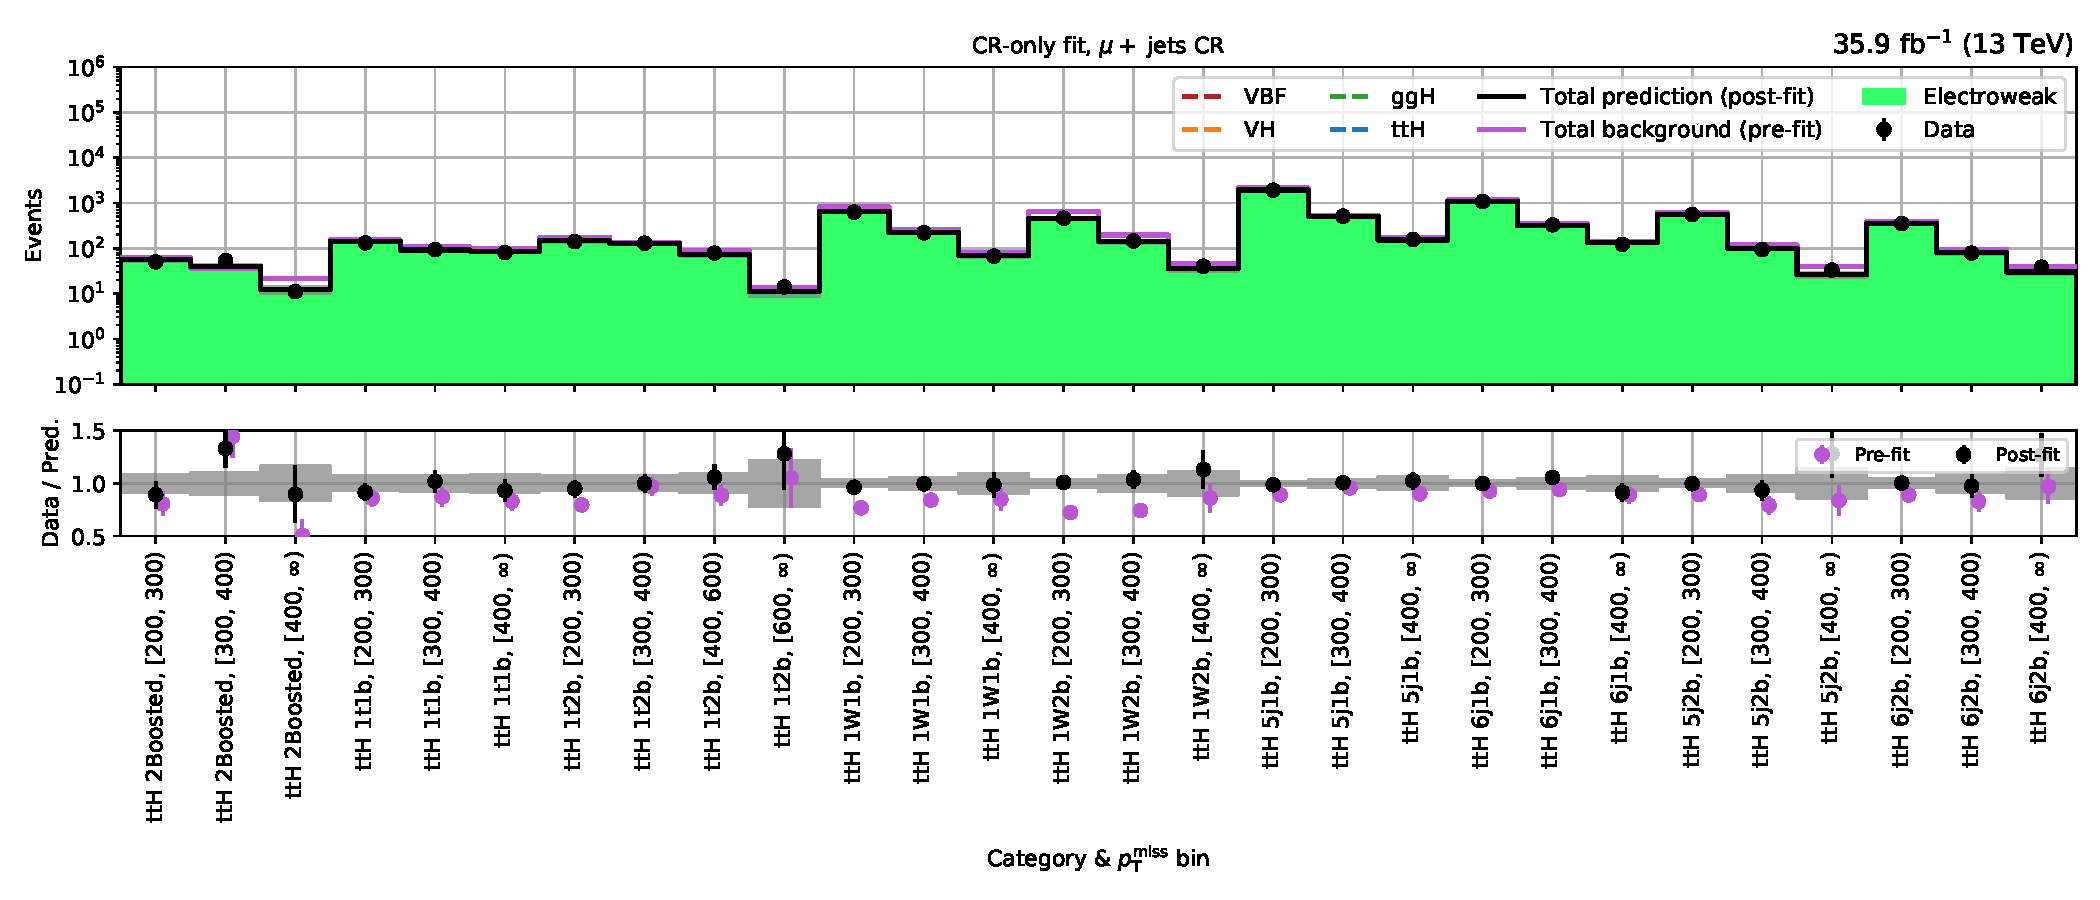
\includegraphics[width=\textwidth]{chapters/higgstoinv/figures/mountain_ranges/2016/ttH/Wmunu_tree_fit_b-abs_values_ttH_cats.pdf}
        \caption{\ttH --- \singleMuCr \gls{CR} (2016)}
    \end{subfigure}

    \begin{subfigure}[b]{0.65\textwidth}
        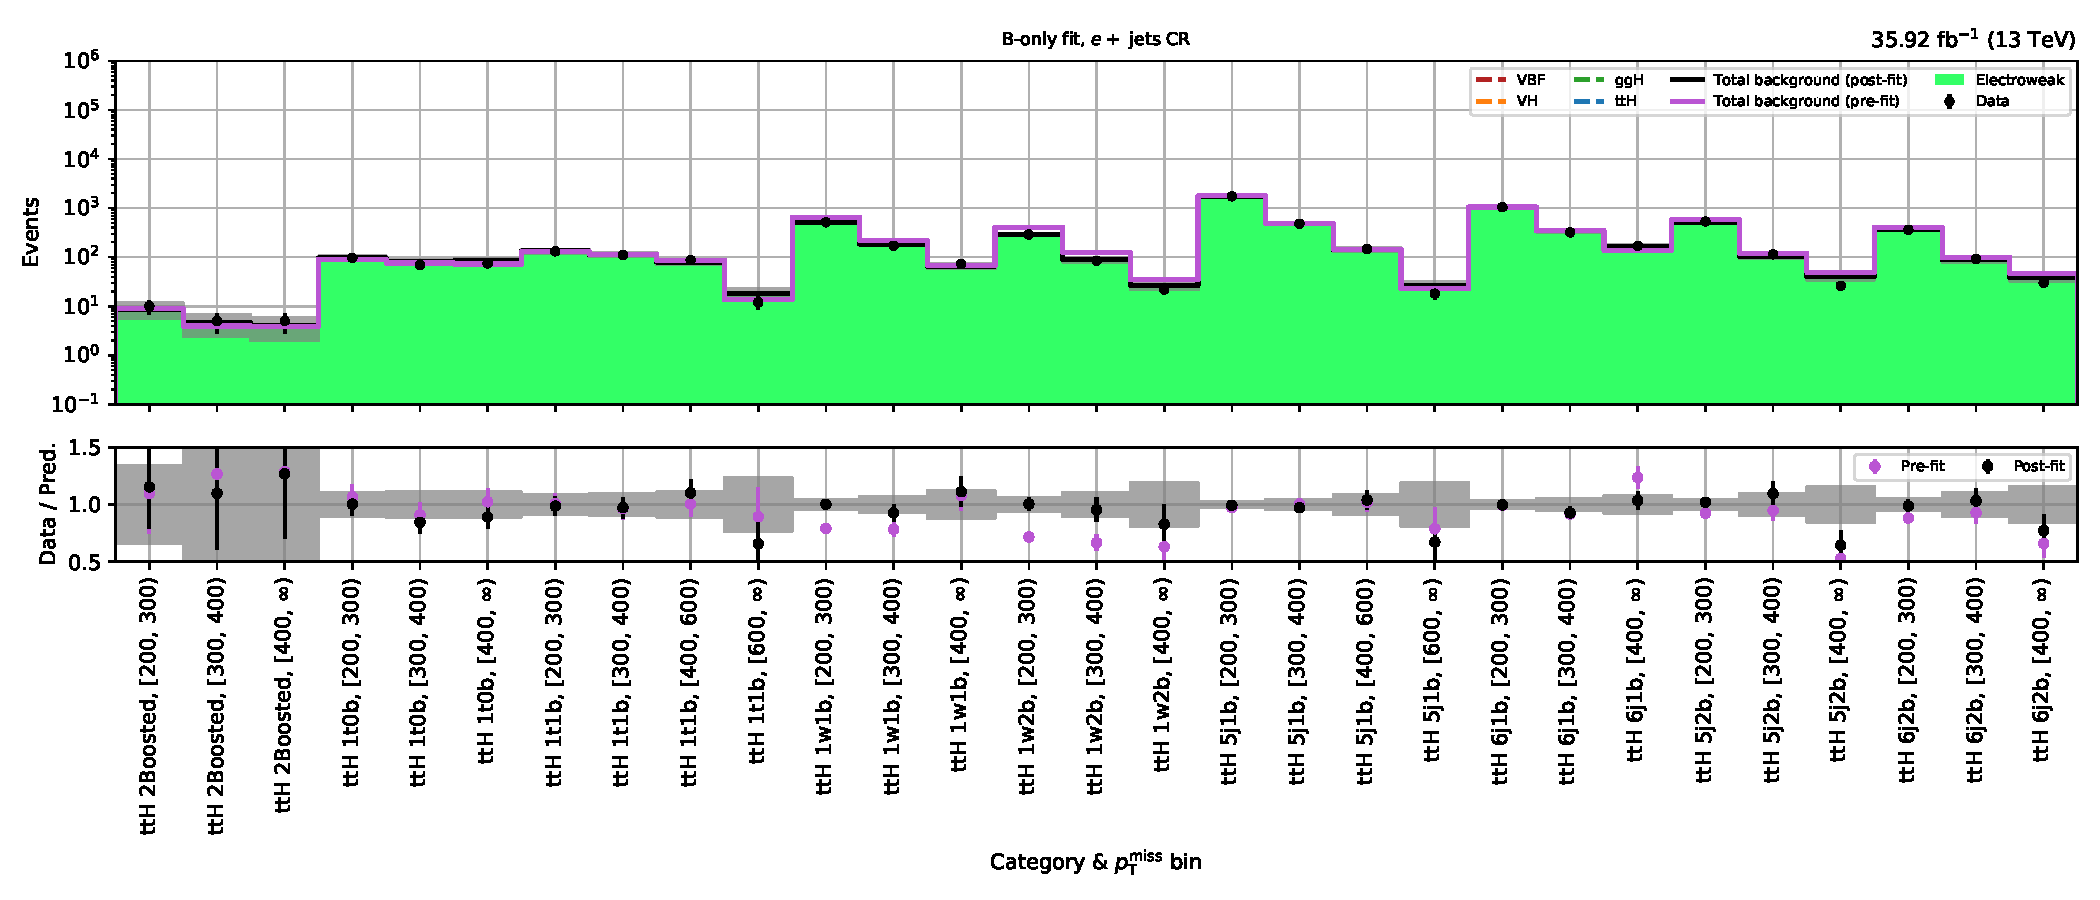
\includegraphics[width=\textwidth]{chapters/higgstoinv/figures/mountain_ranges/2016/ttH/Wenu_tree_fit_b-abs_values_ttH_cats.pdf}
        \caption{\ttH --- \singleEleCr \gls{CR} (2016)}
    \end{subfigure}

    \begin{subfigure}[b]{0.65\textwidth}
        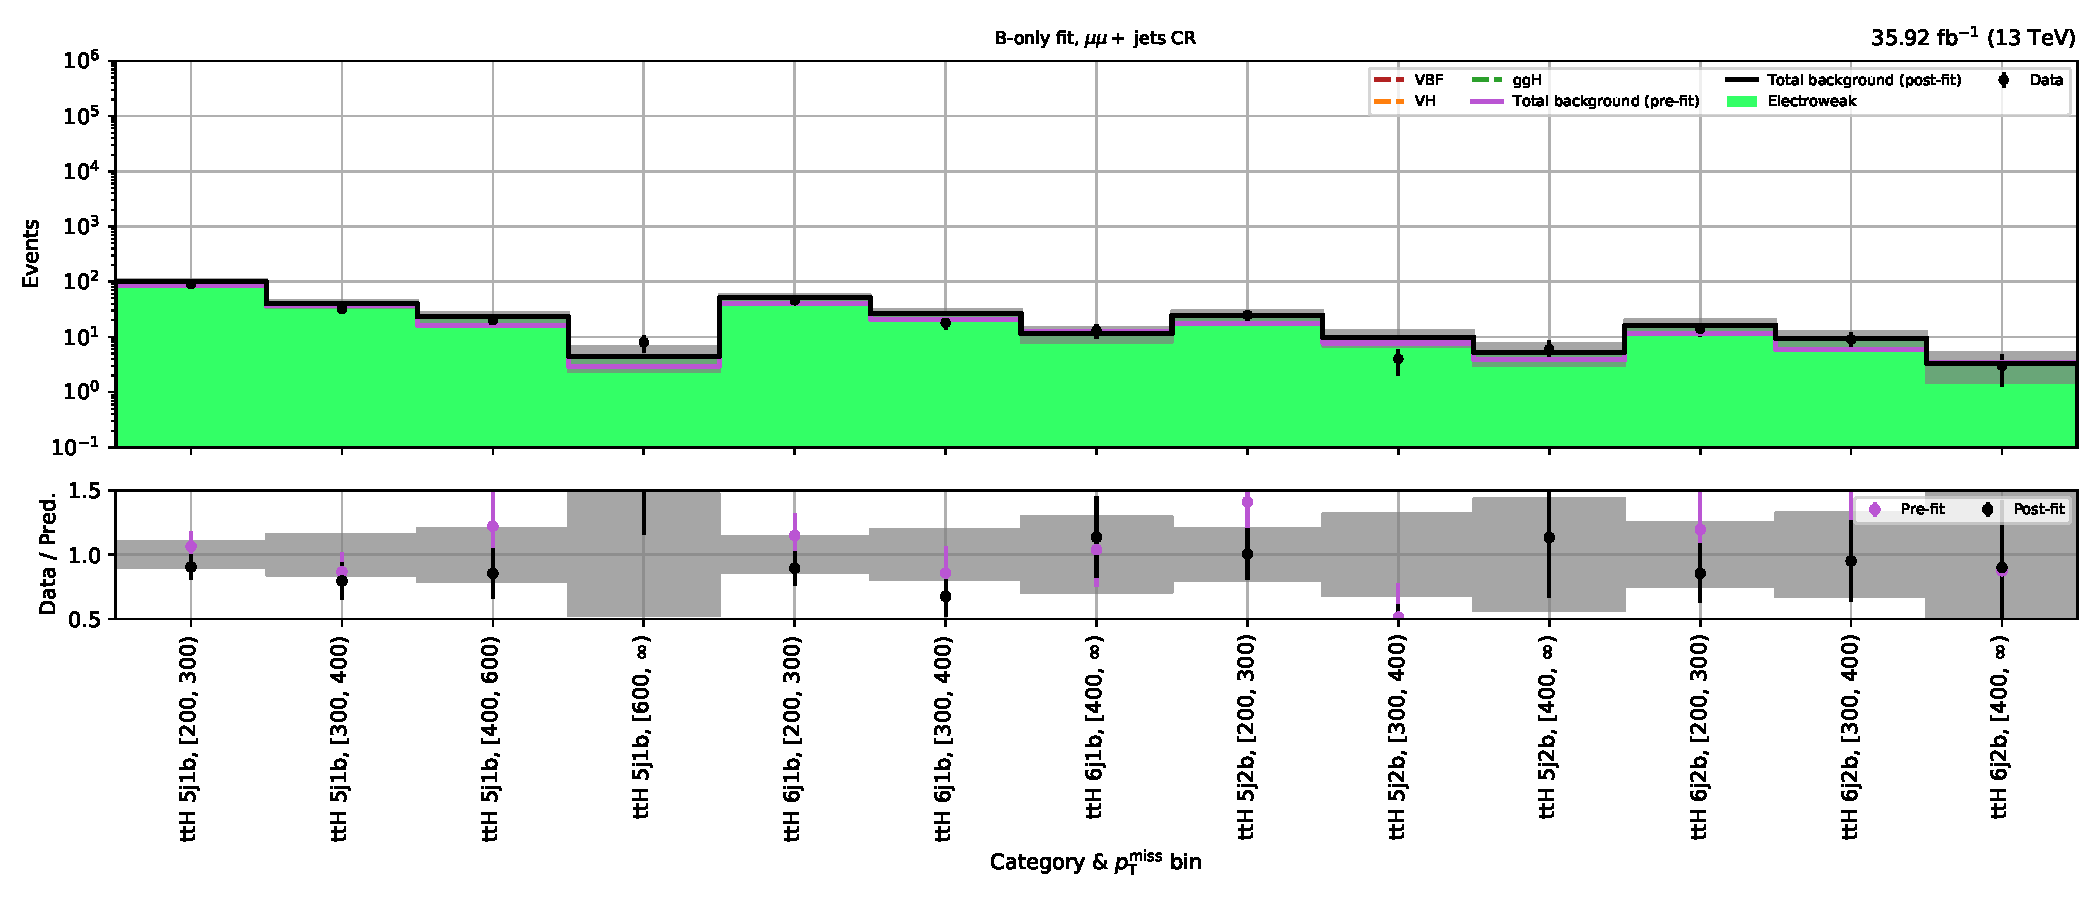
\includegraphics[width=\textwidth]{chapters/higgstoinv/figures/mountain_ranges/2016/ttH/Zmumu_tree_fit_b-abs_values_ttH_cats.pdf}
        \caption{\ttH --- \doubleMuCr \gls{CR} (2016)}
    \end{subfigure}

    \begin{subfigure}[b]{0.65\textwidth}
        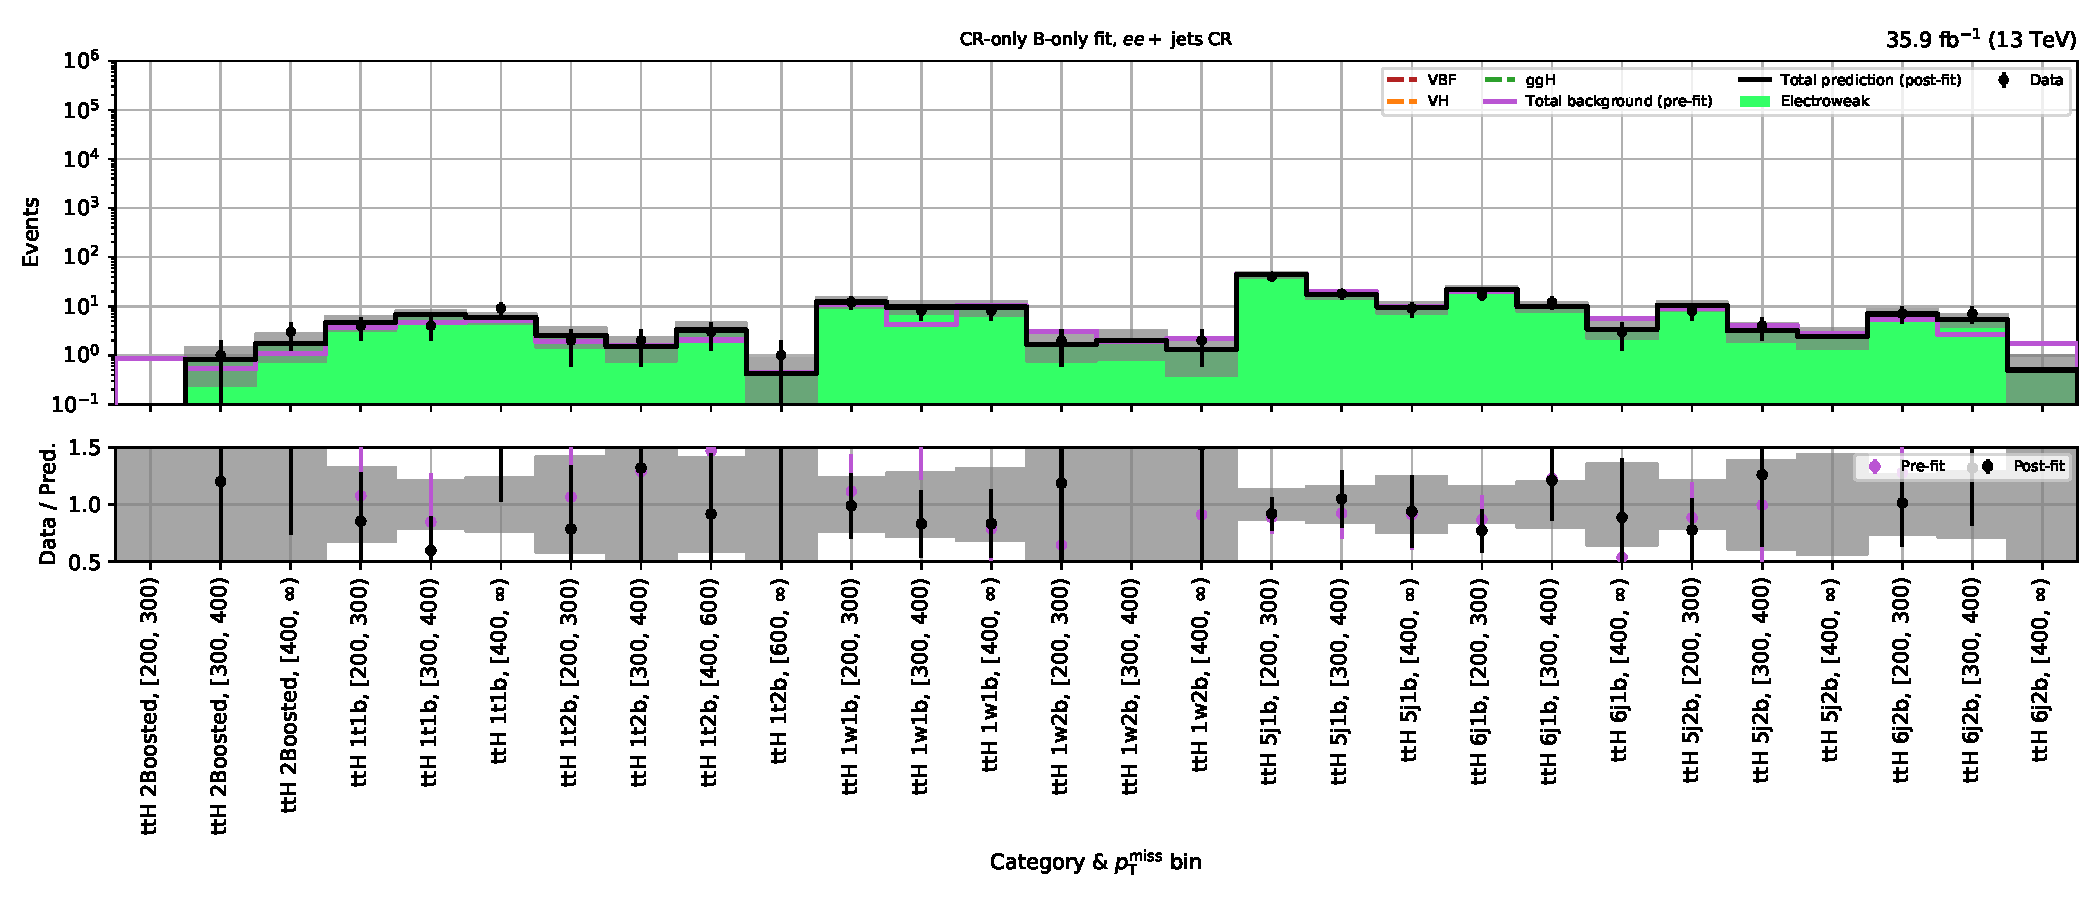
\includegraphics[width=\textwidth]{chapters/higgstoinv/figures/mountain_ranges/2016/ttH/Zee_tree_fit_b-abs_values_ttH_cats.pdf}
        \caption{\ttH --- \doubleEleCr \gls{CR} (2016)}
    \end{subfigure}
    \caption[Post-fit yields for each \ttH subcategory and \ptmiss bin in the lepton control regions for the 2016 dataset]{Post-fit yields for each \ttH subcategory and \ptmiss bin in the lepton \glspl{CR} for the 2016 dataset. The total background pre-fit and post-fit is compared to data in the lower panel of each subfigure.}
    \label{fig:htoinv_mountain_range_ttH_2016_CRs}
\end{figure}

\begin{figure}[htbp]
    \centering
    \begin{subfigure}[b]{0.65\textwidth}
        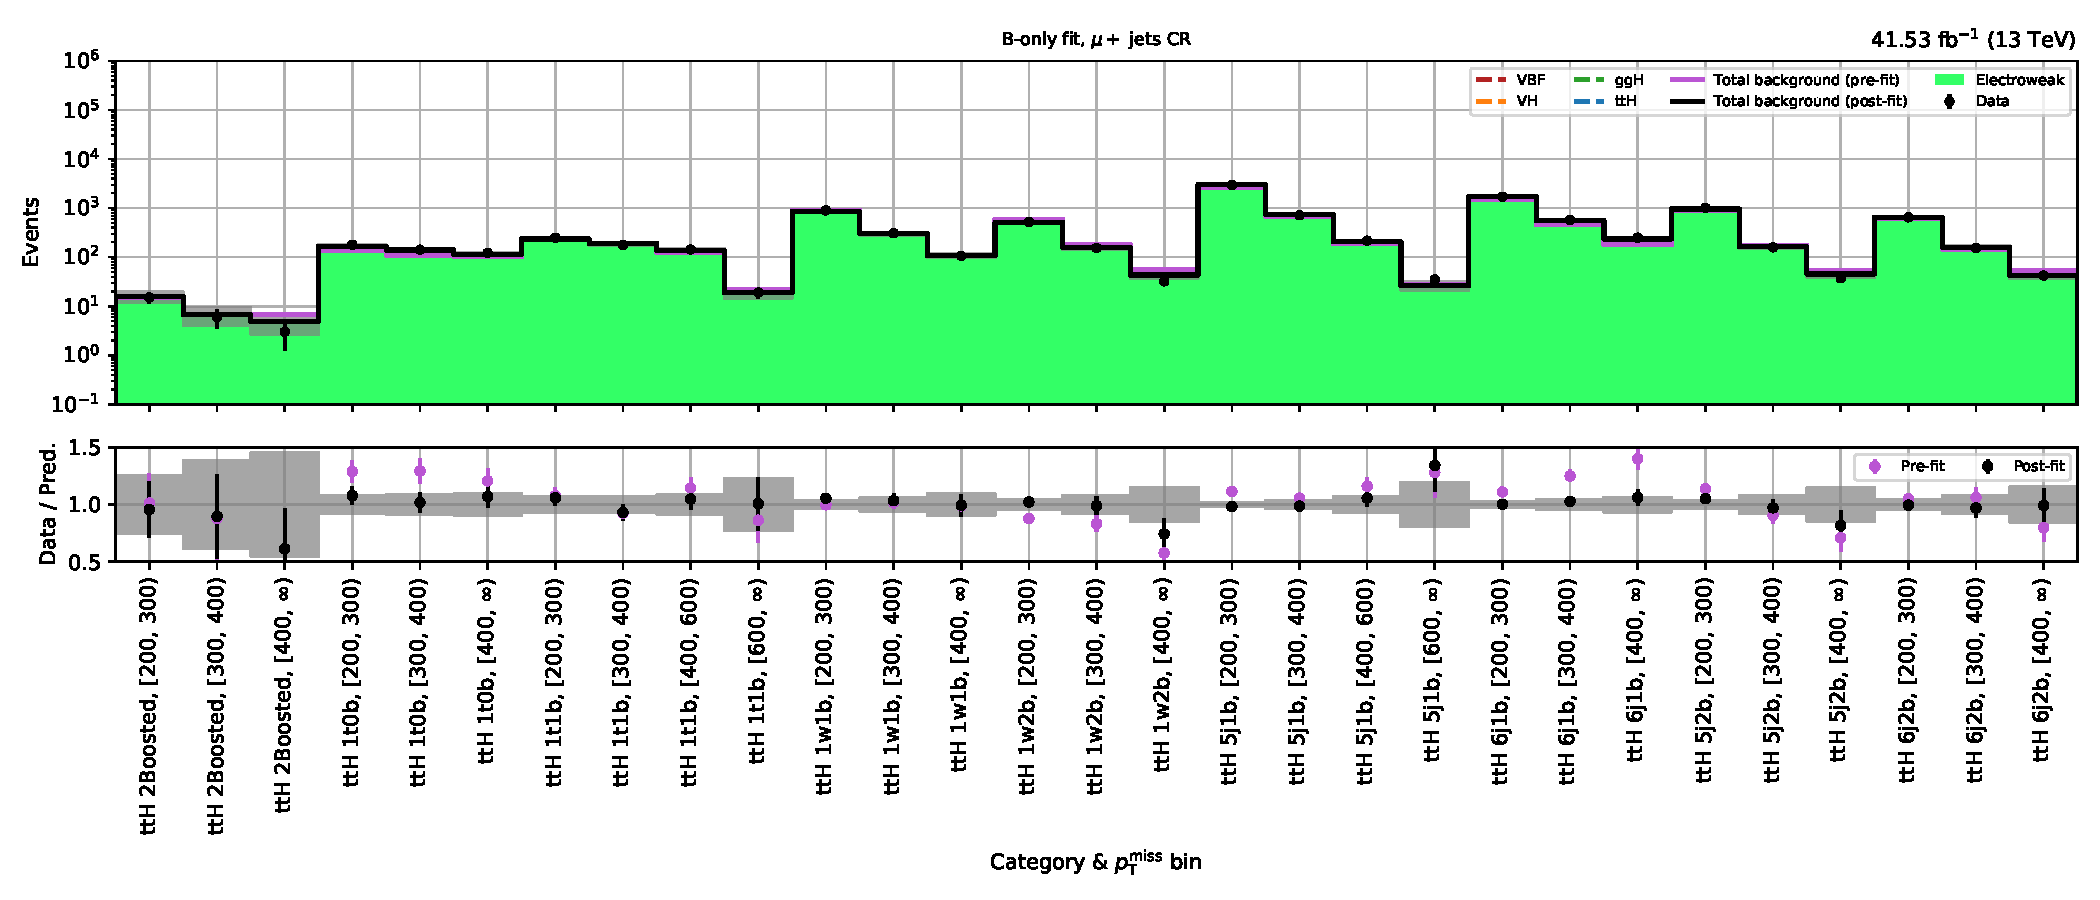
\includegraphics[width=\textwidth]{chapters/higgstoinv/figures/mountain_ranges/2017/ttH/Wmunu_tree_fit_b-abs_values_ttH_cats.pdf}
        \caption{\ttH --- \singleMuCr \gls{CR} (2017)}
    \end{subfigure}

    \begin{subfigure}[b]{0.65\textwidth}
        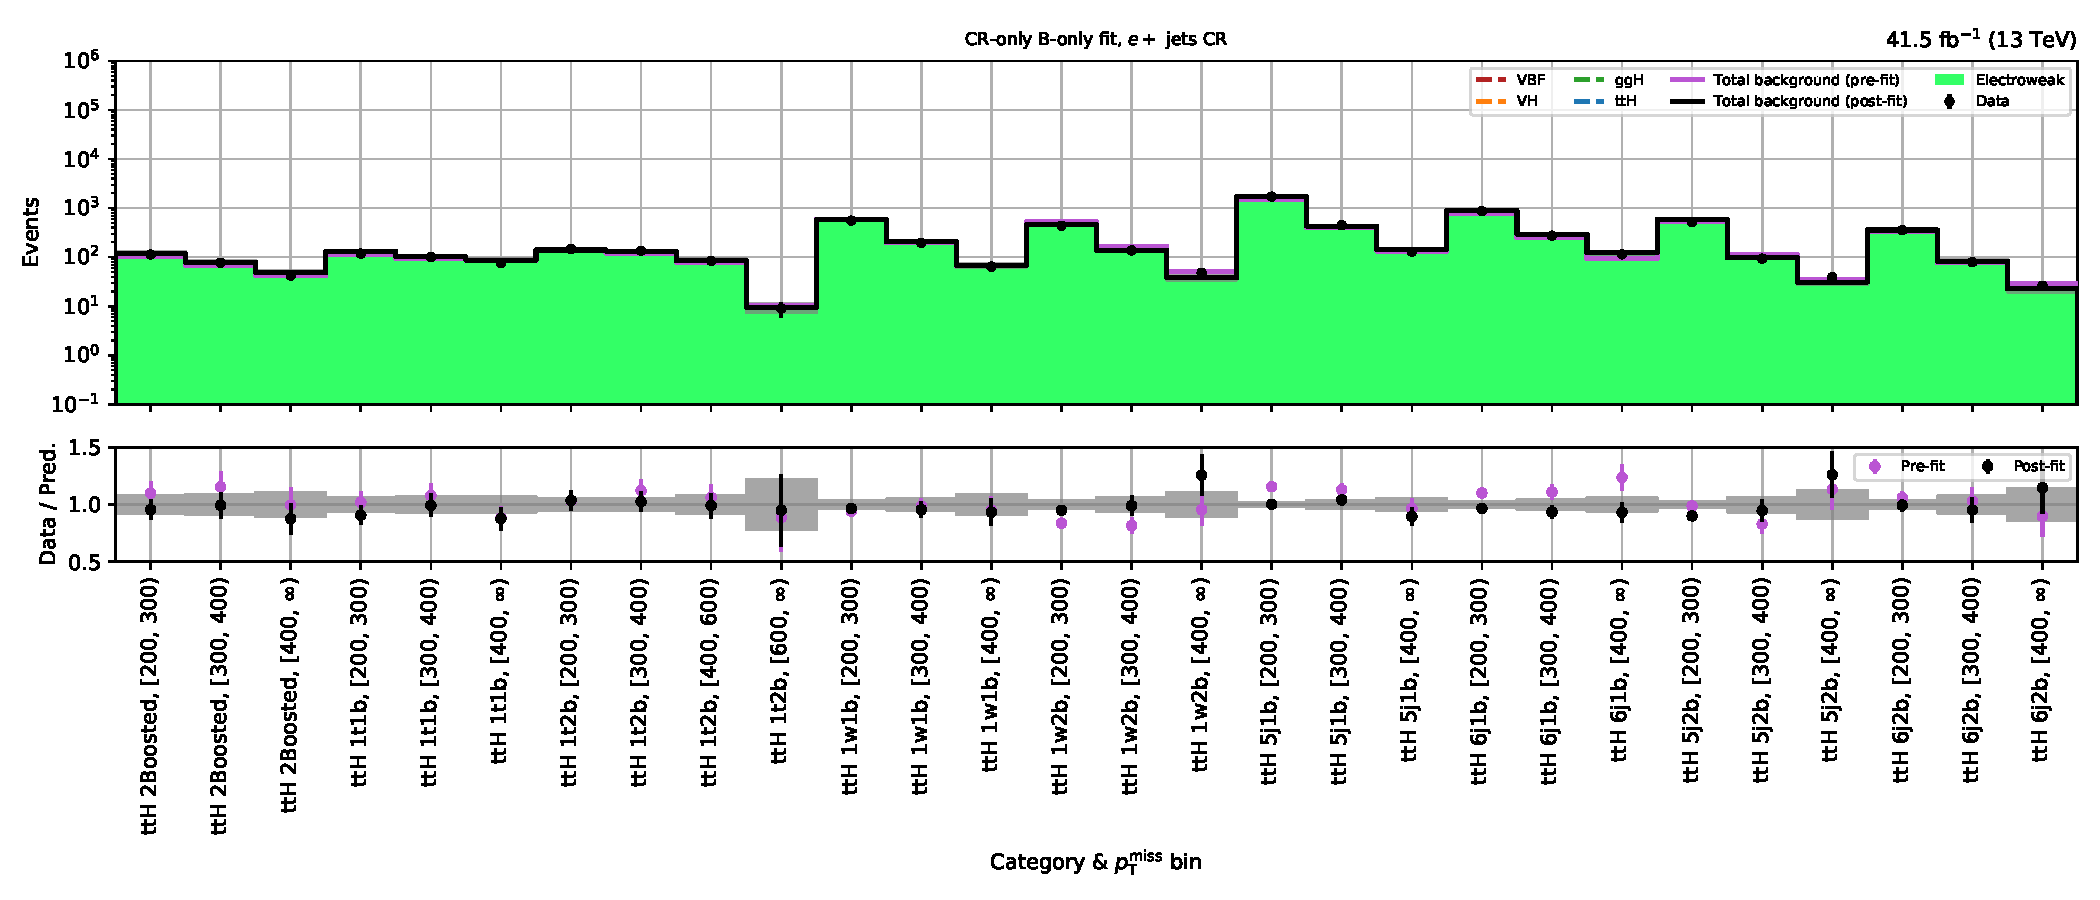
\includegraphics[width=\textwidth]{chapters/higgstoinv/figures/mountain_ranges/2017/ttH/Wenu_tree_fit_b-abs_values_ttH_cats.pdf}
        \caption{\ttH --- \singleEleCr \gls{CR} (2017)}
    \end{subfigure}

    \begin{subfigure}[b]{0.65\textwidth}
        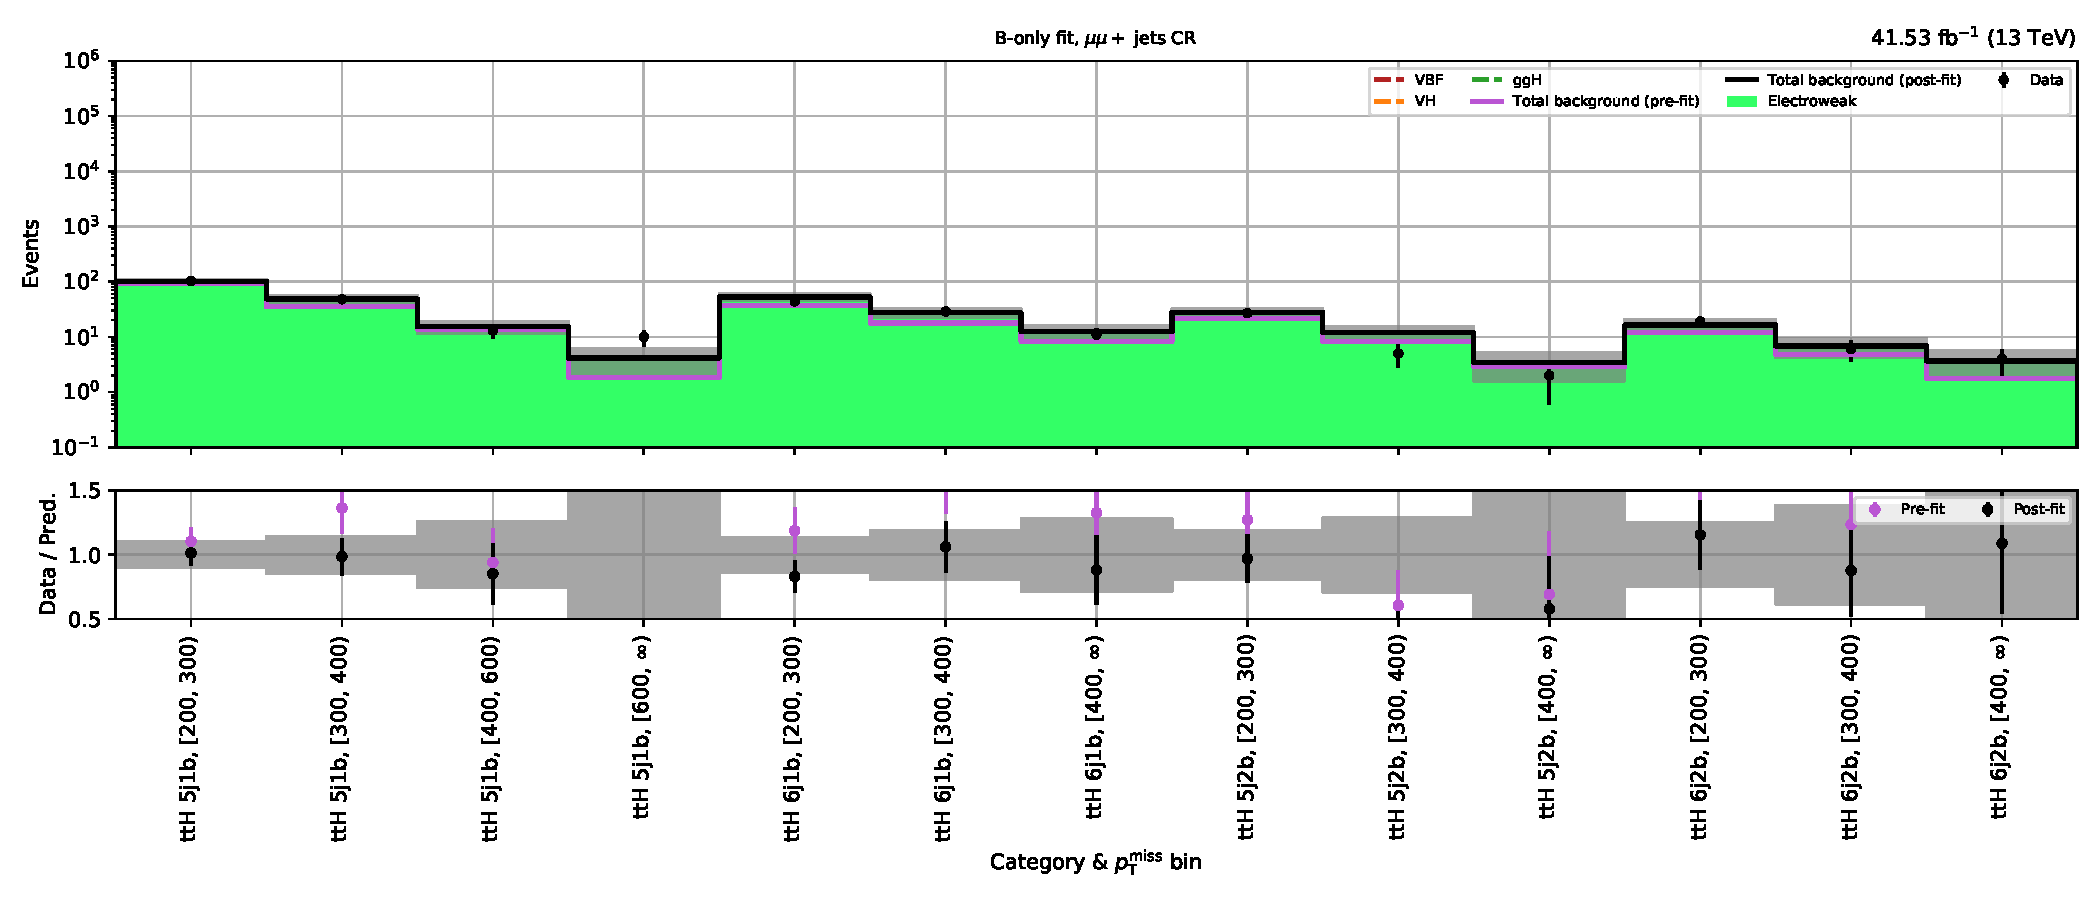
\includegraphics[width=\textwidth]{chapters/higgstoinv/figures/mountain_ranges/2017/ttH/Zmumu_tree_fit_b-abs_values_ttH_cats.pdf}
        \caption{\ttH --- \doubleMuCr \gls{CR} (2017)}
    \end{subfigure}

    \begin{subfigure}[b]{0.65\textwidth}
        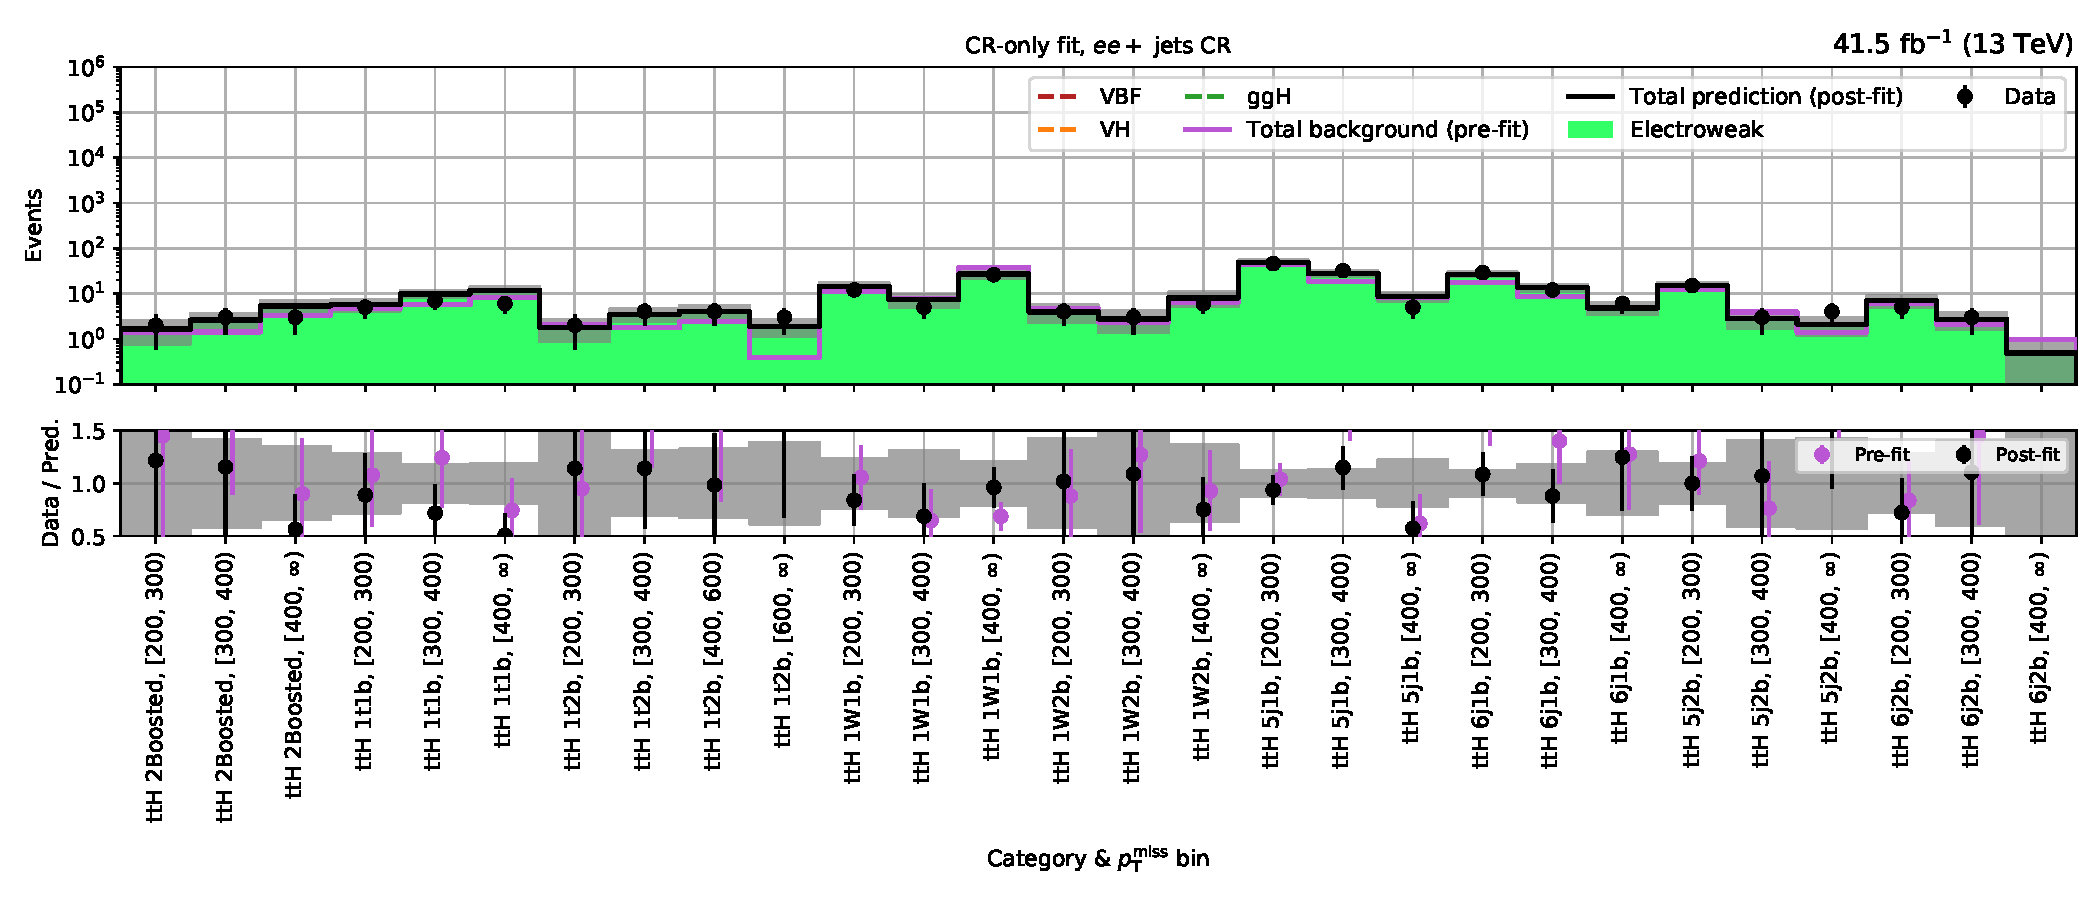
\includegraphics[width=\textwidth]{chapters/higgstoinv/figures/mountain_ranges/2017/ttH/Zee_tree_fit_b-abs_values_ttH_cats.pdf}
        \caption{\ttH --- \doubleEleCr \gls{CR} (2017)}
    \end{subfigure}
    \caption[Post-fit yields for each \ttH subcategory and \ptmiss bin in the lepton control regions for the 2017 dataset]{Post-fit yields for each \ttH subcategory and \ptmiss bin in the lepton \glspl{CR} for the 2017 dataset. The total background pre-fit and post-fit is compared to data in the lower panel of each subfigure.}
    \label{fig:htoinv_mountain_range_ttH_2017_CRs}
\end{figure}

\begin{figure}[htbp]
    \centering
    \begin{subfigure}[b]{0.65\textwidth}
        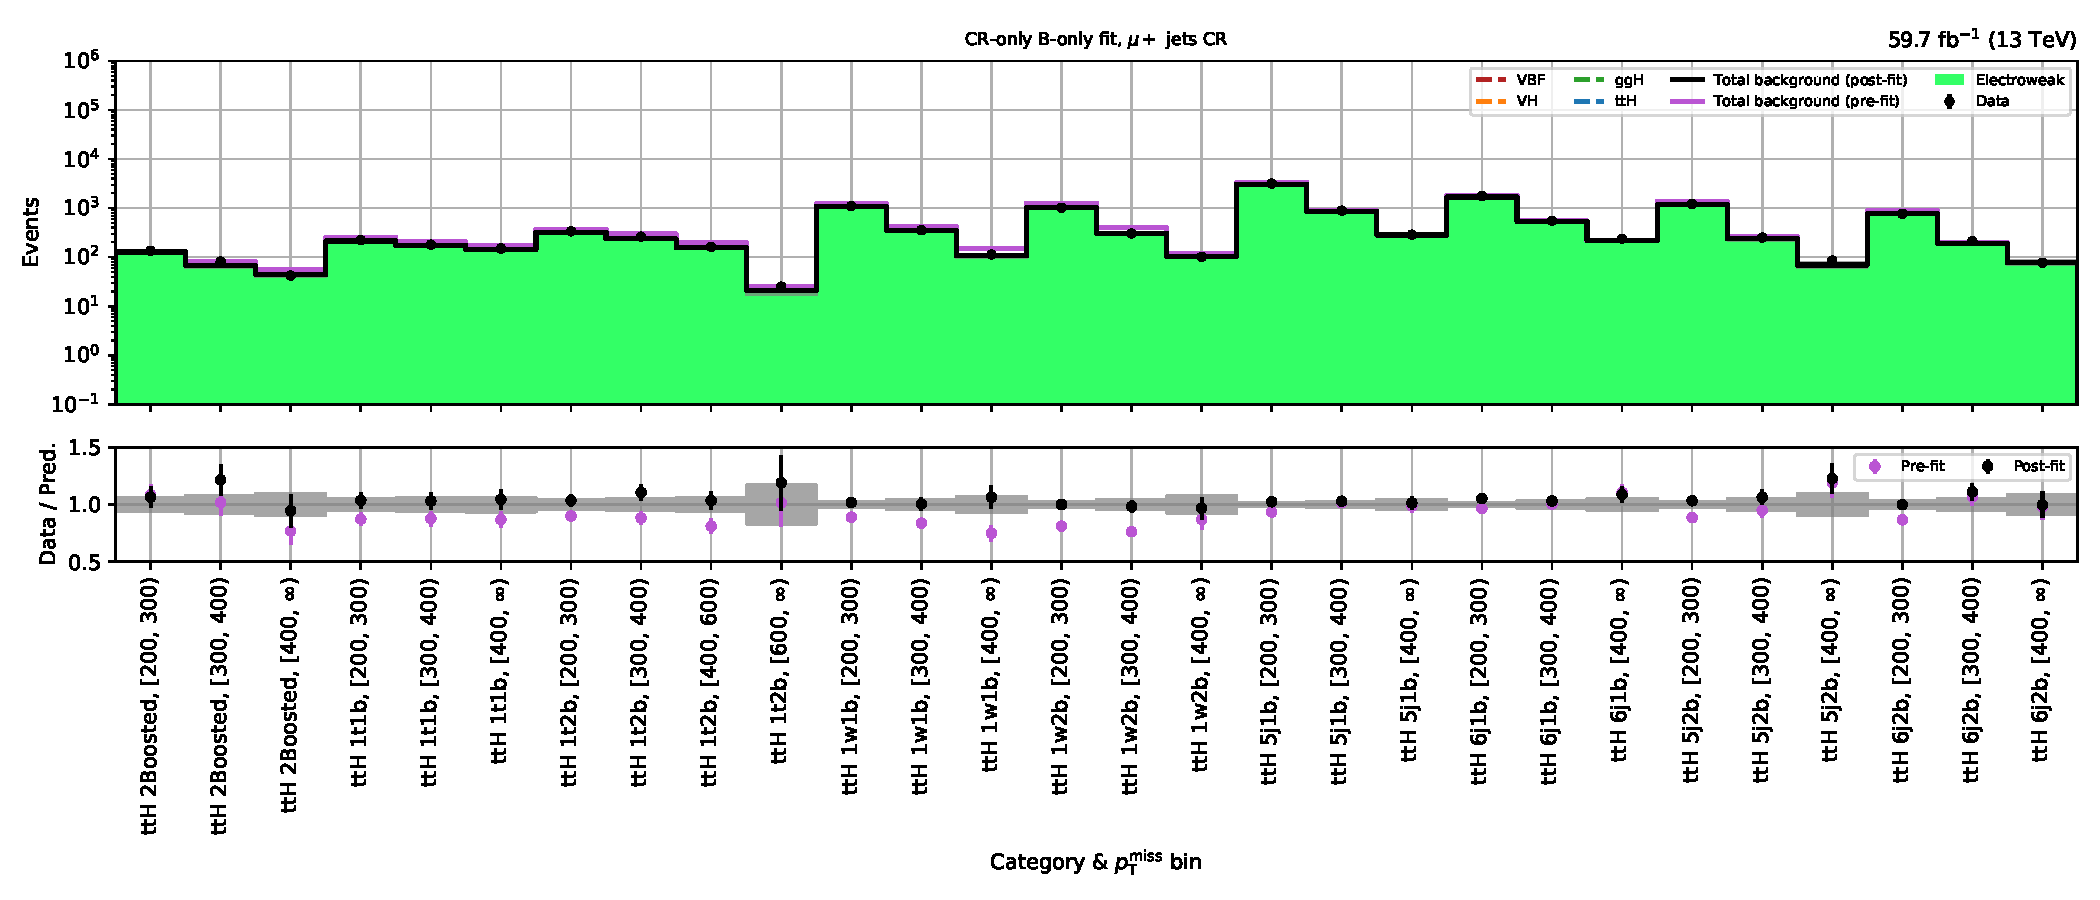
\includegraphics[width=\textwidth]{chapters/higgstoinv/figures/mountain_ranges/2018/ttH/Wmunu_tree_fit_b-abs_values_ttH_cats.pdf}
        \caption{\ttH --- \singleMuCr \gls{CR} (2018)}
    \end{subfigure}

    \begin{subfigure}[b]{0.65\textwidth}
        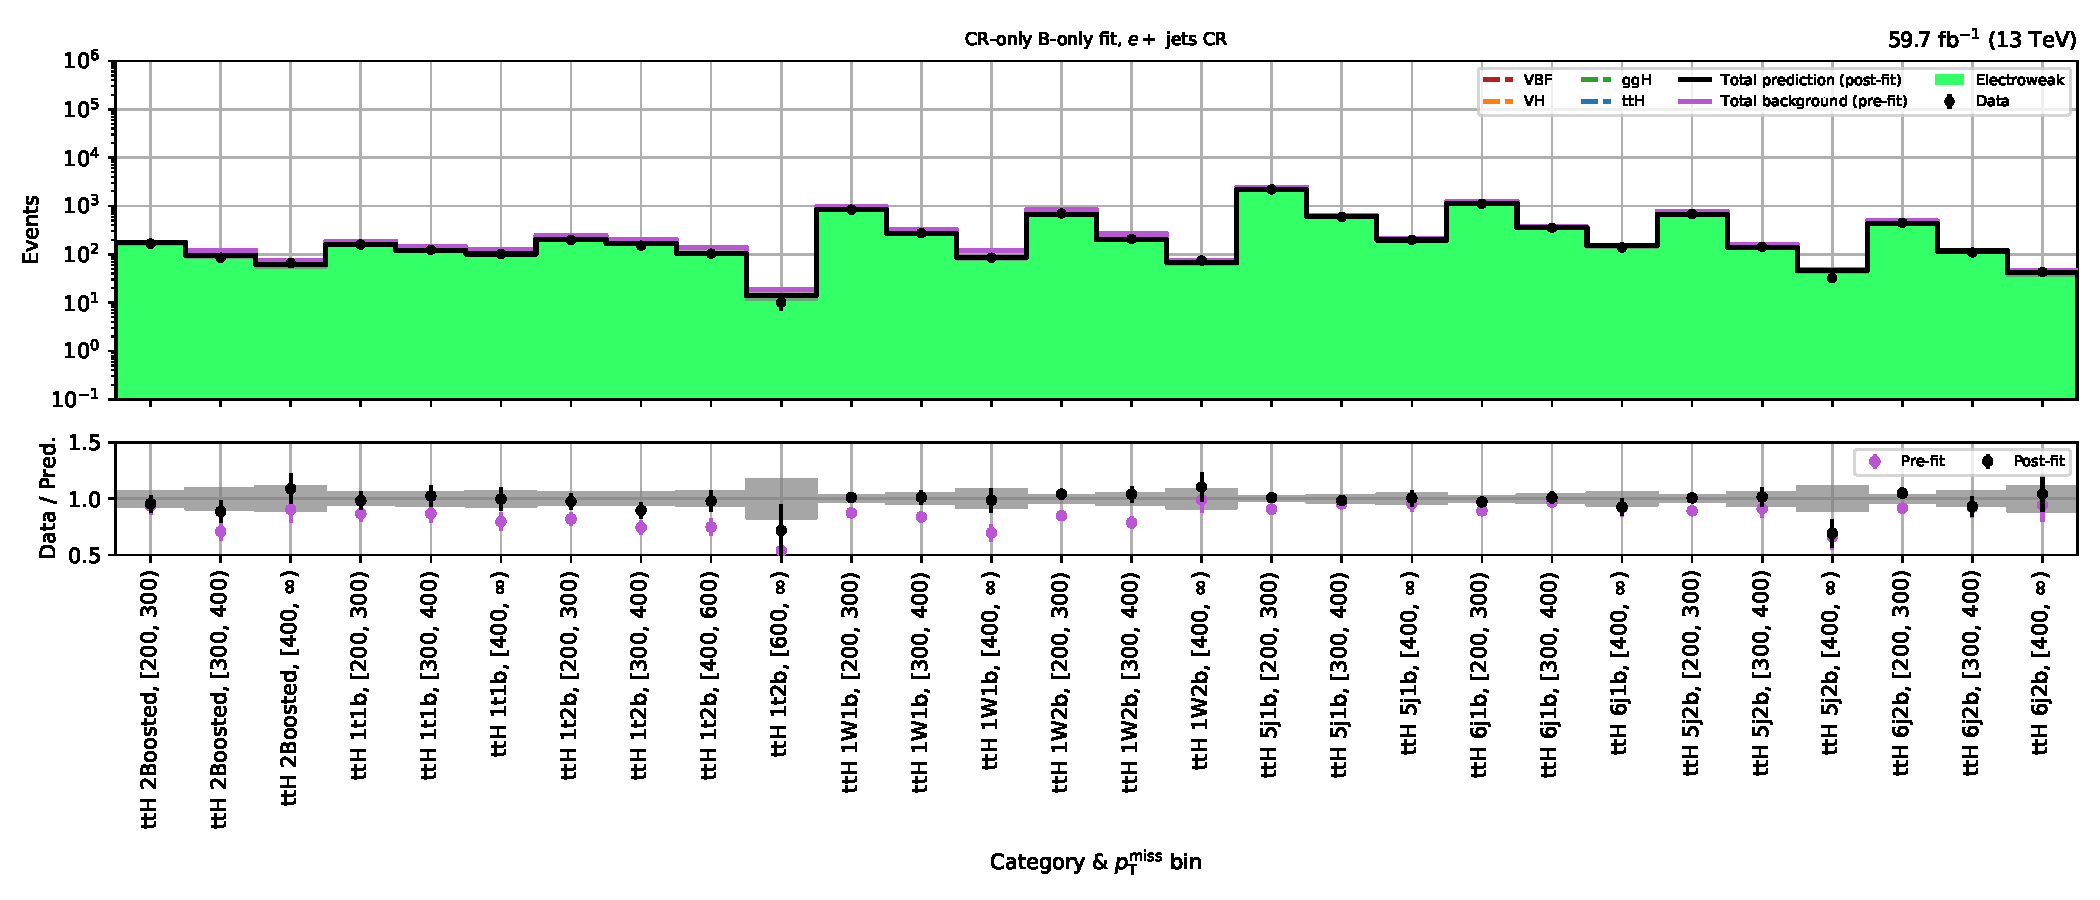
\includegraphics[width=\textwidth]{chapters/higgstoinv/figures/mountain_ranges/2018/ttH/Wenu_tree_fit_b-abs_values_ttH_cats.pdf}
        \caption{\ttH --- \singleEleCr \gls{CR} (2018)}
    \end{subfigure}

    \begin{subfigure}[b]{0.65\textwidth}
        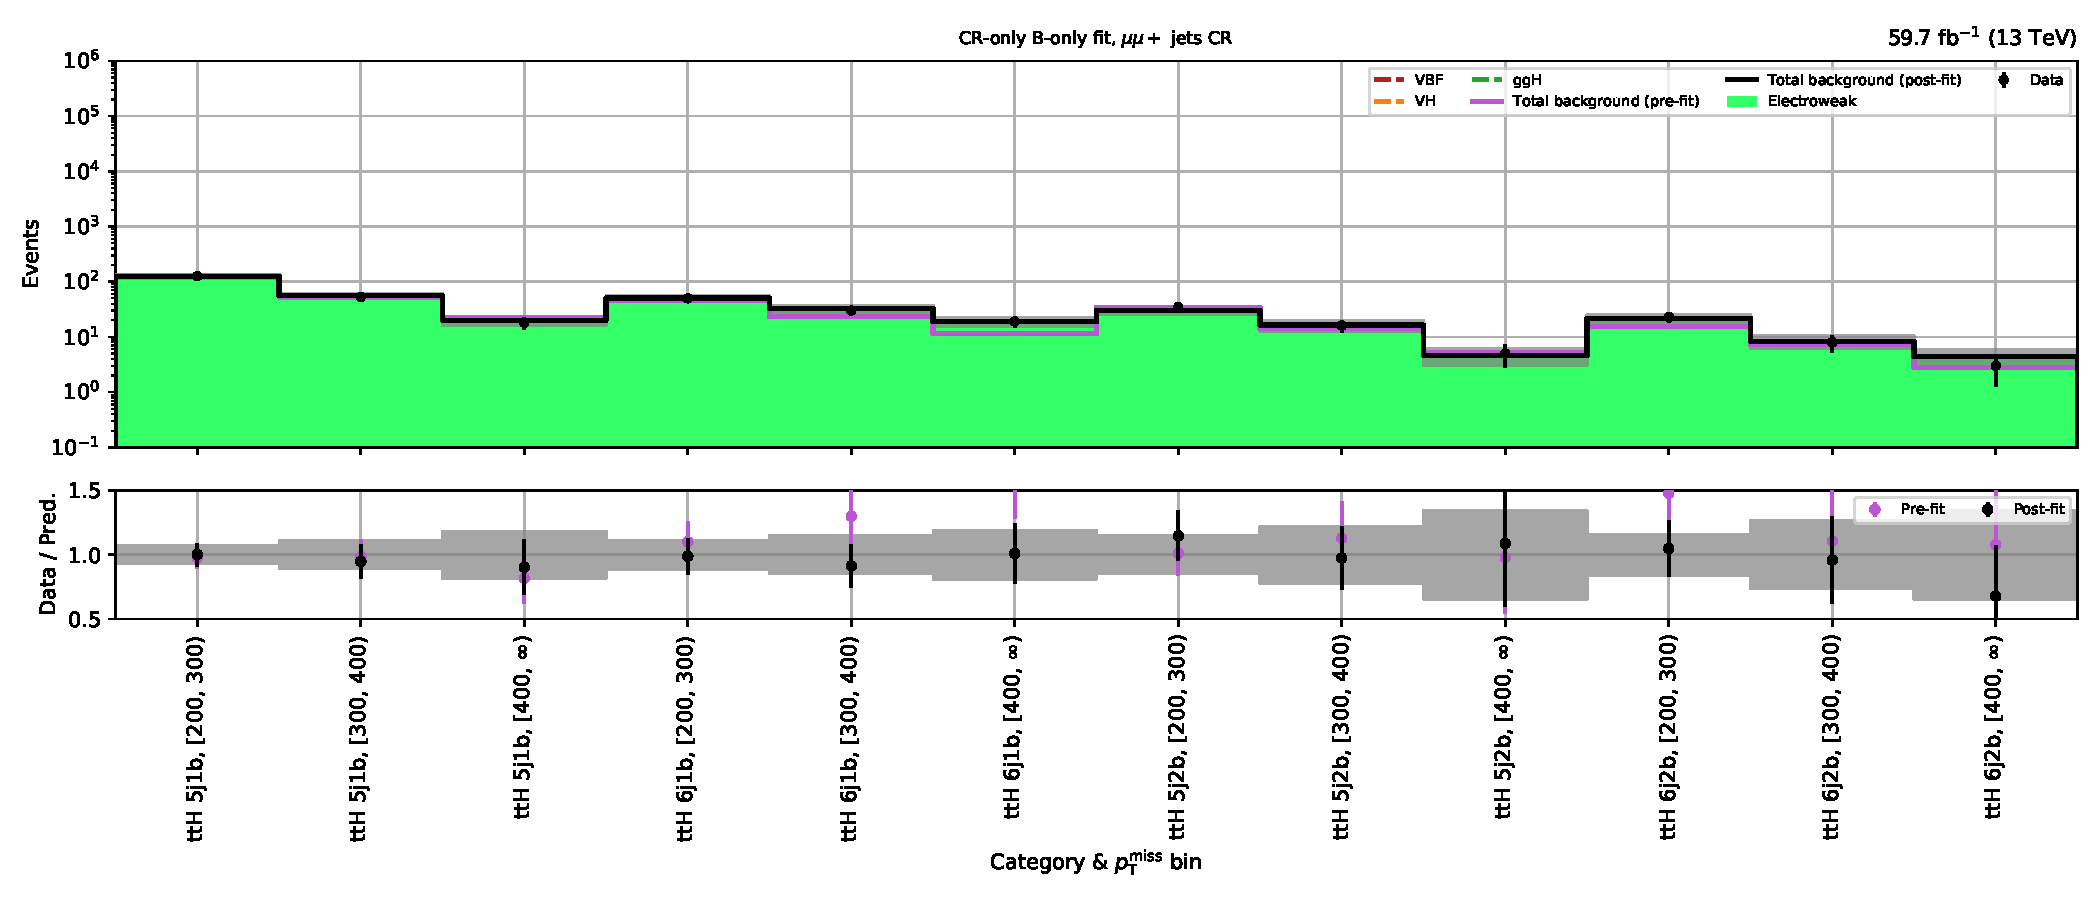
\includegraphics[width=\textwidth]{chapters/higgstoinv/figures/mountain_ranges/2018/ttH/Zmumu_tree_fit_b-abs_values_ttH_cats.pdf}
        \caption{\ttH --- \doubleMuCr \gls{CR} (2018)}
    \end{subfigure}

    \begin{subfigure}[b]{0.65\textwidth}
        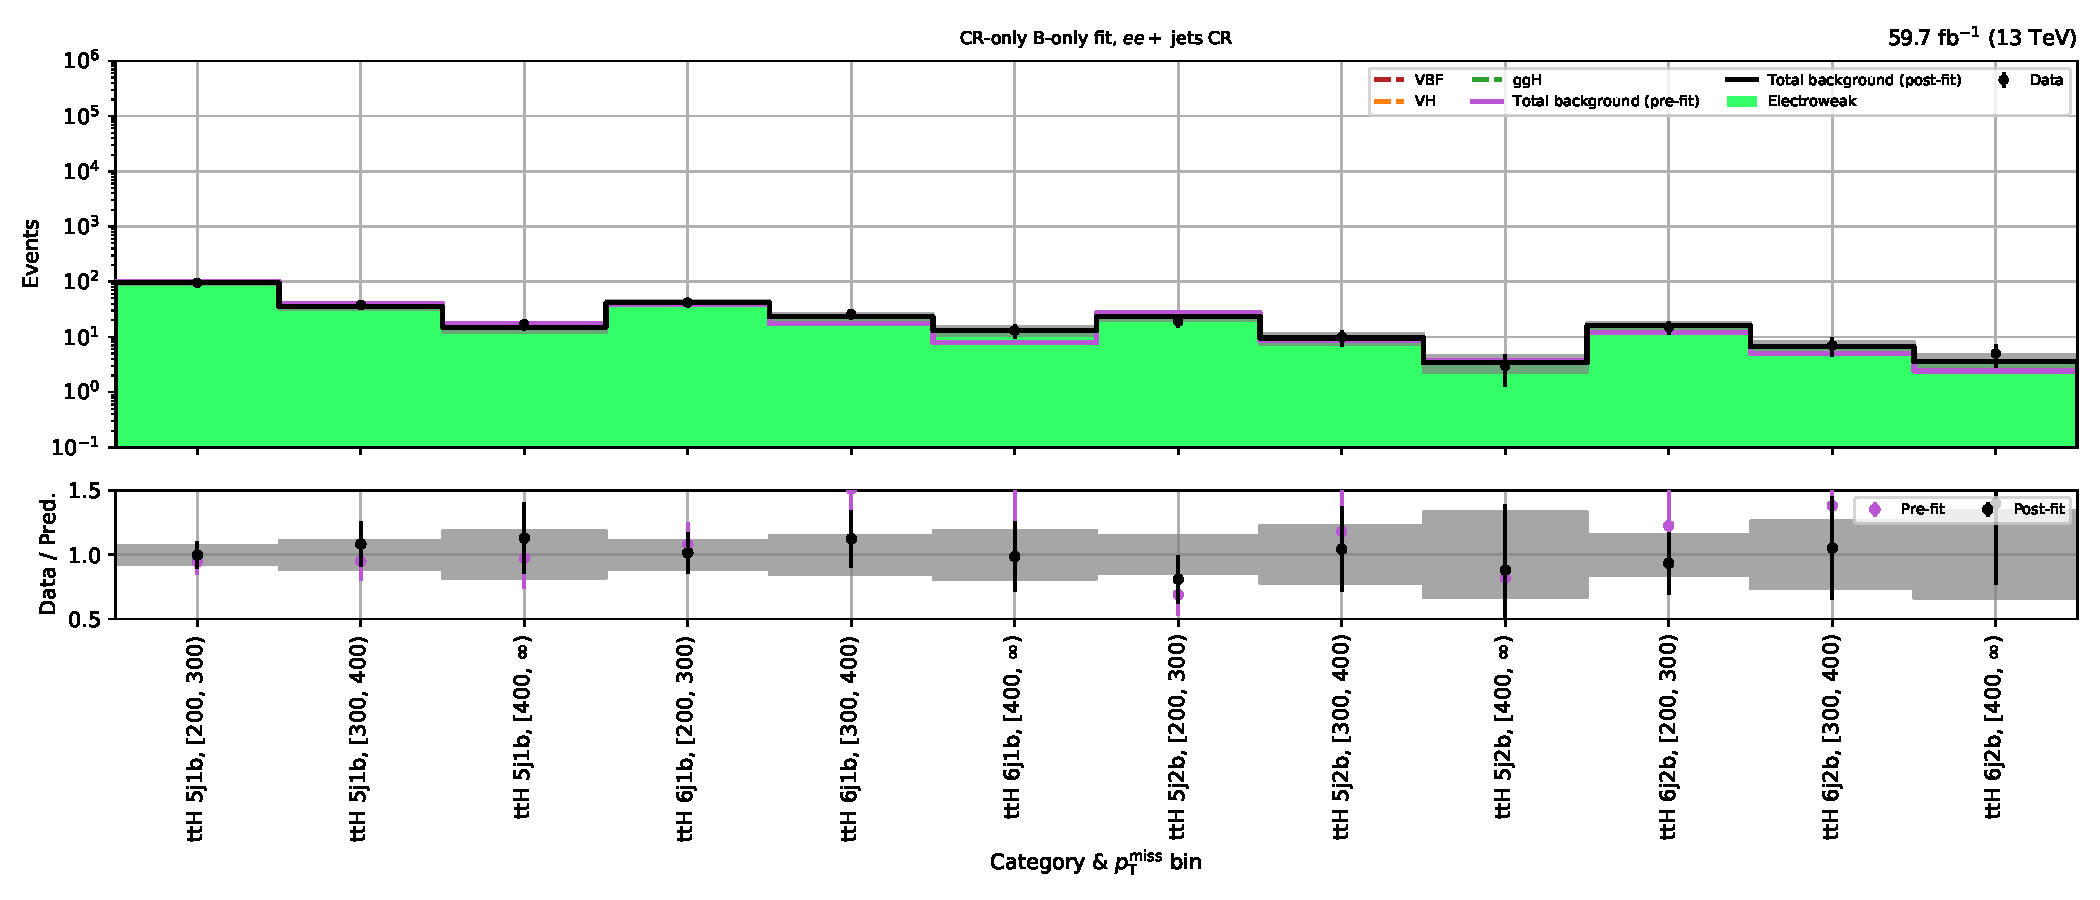
\includegraphics[width=\textwidth]{chapters/higgstoinv/figures/mountain_ranges/2018/ttH/Zee_tree_fit_b-abs_values_ttH_cats.pdf}
        \caption{\ttH --- \doubleEleCr \gls{CR} (2018)}
    \end{subfigure}
    \caption[Post-fit yields for each \ttH subcategory and \ptmiss bin in the lepton control regions for the 2018 dataset]{Post-fit yields for each \ttH subcategory and \ptmiss bin in the lepton \glspl{CR} for the 2018 dataset. The total background pre-fit and post-fit is compared to data in the lower panel of each subfigure.}
    \label{fig:htoinv_mountain_range_ttH_2018_CRs}
\end{figure}

\clearpage


%=========================================================


\section{Post-fit distributions of the control regions in the \texorpdfstring{\VH}{VH} category}
\label{sec:pre_post_fit_plots_VH_CRs}

\begin{figure}[htbp]
    \centering
    \begin{subfigure}[b]{0.49\textwidth}
        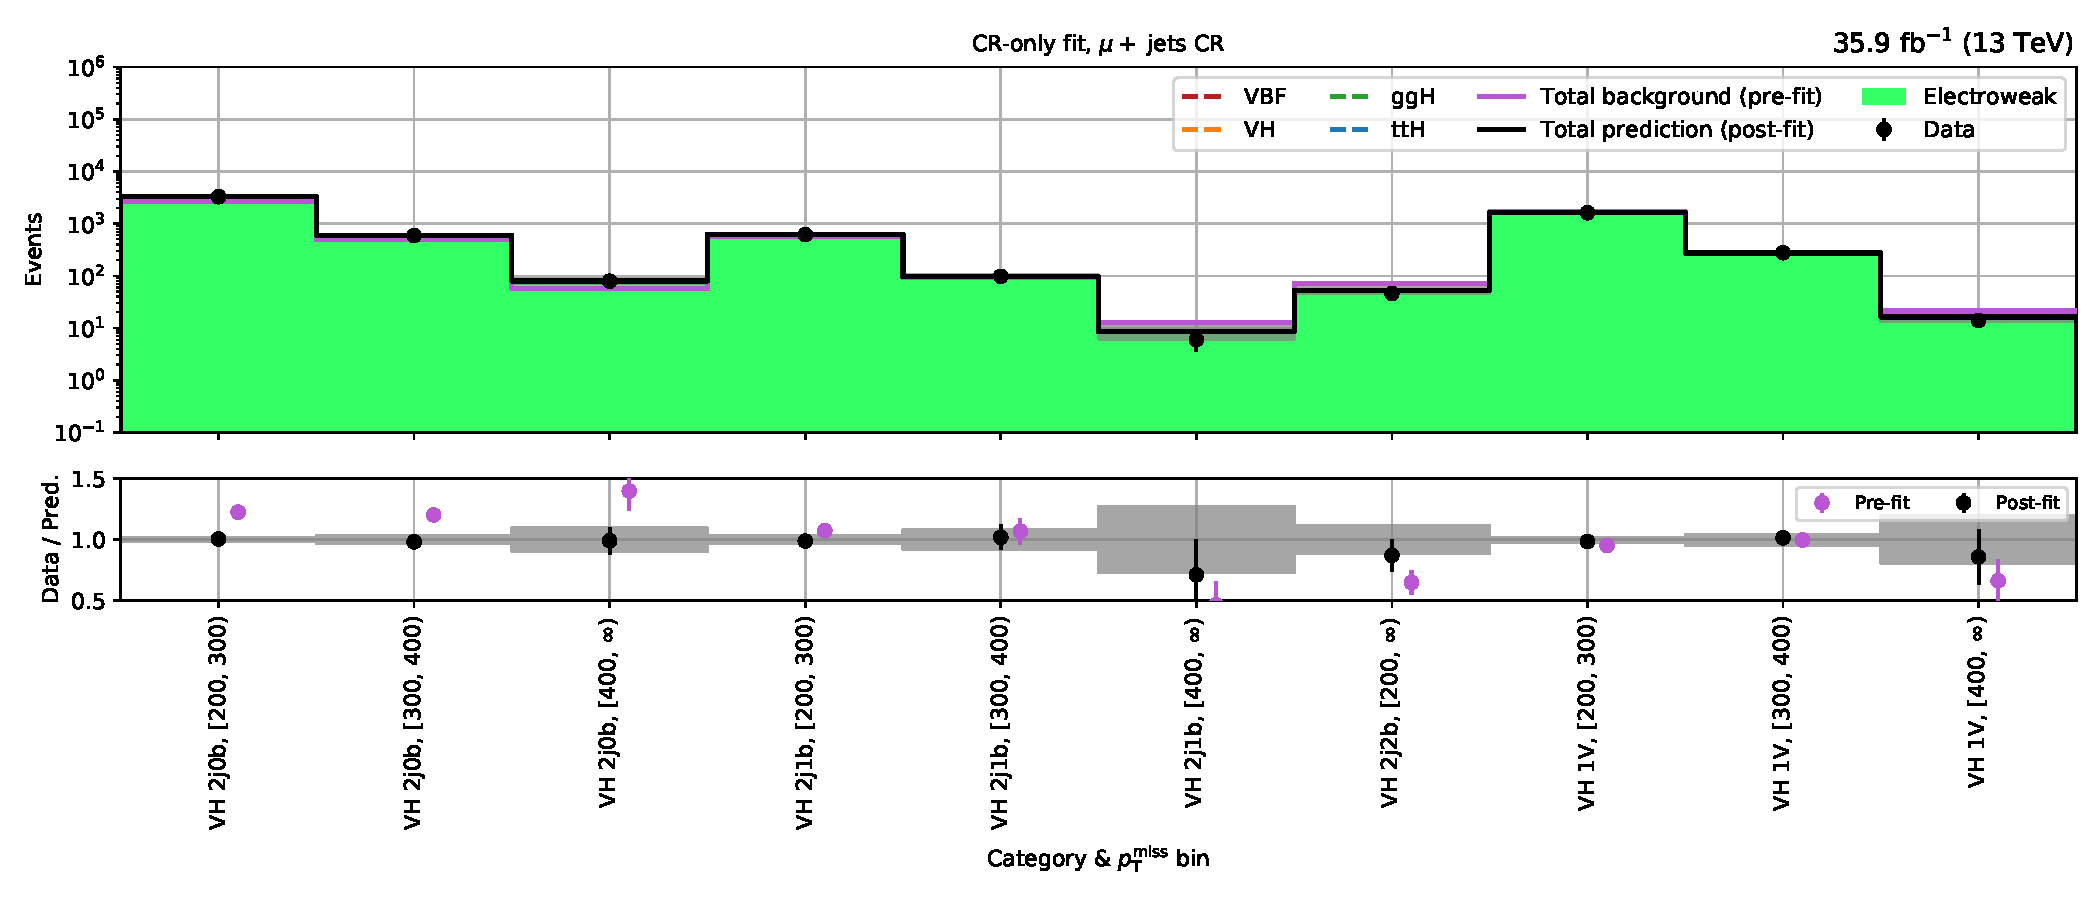
\includegraphics[width=\textwidth]{chapters/higgstoinv/figures/mountain_ranges/2016/VH/Wmunu_tree_fit_b-abs_values_VH_cats.pdf}
        \caption{\VH --- \singleMuCr \gls{CR} (2016)}
    \end{subfigure}
    \hfill
    \begin{subfigure}[b]{0.49\textwidth}
        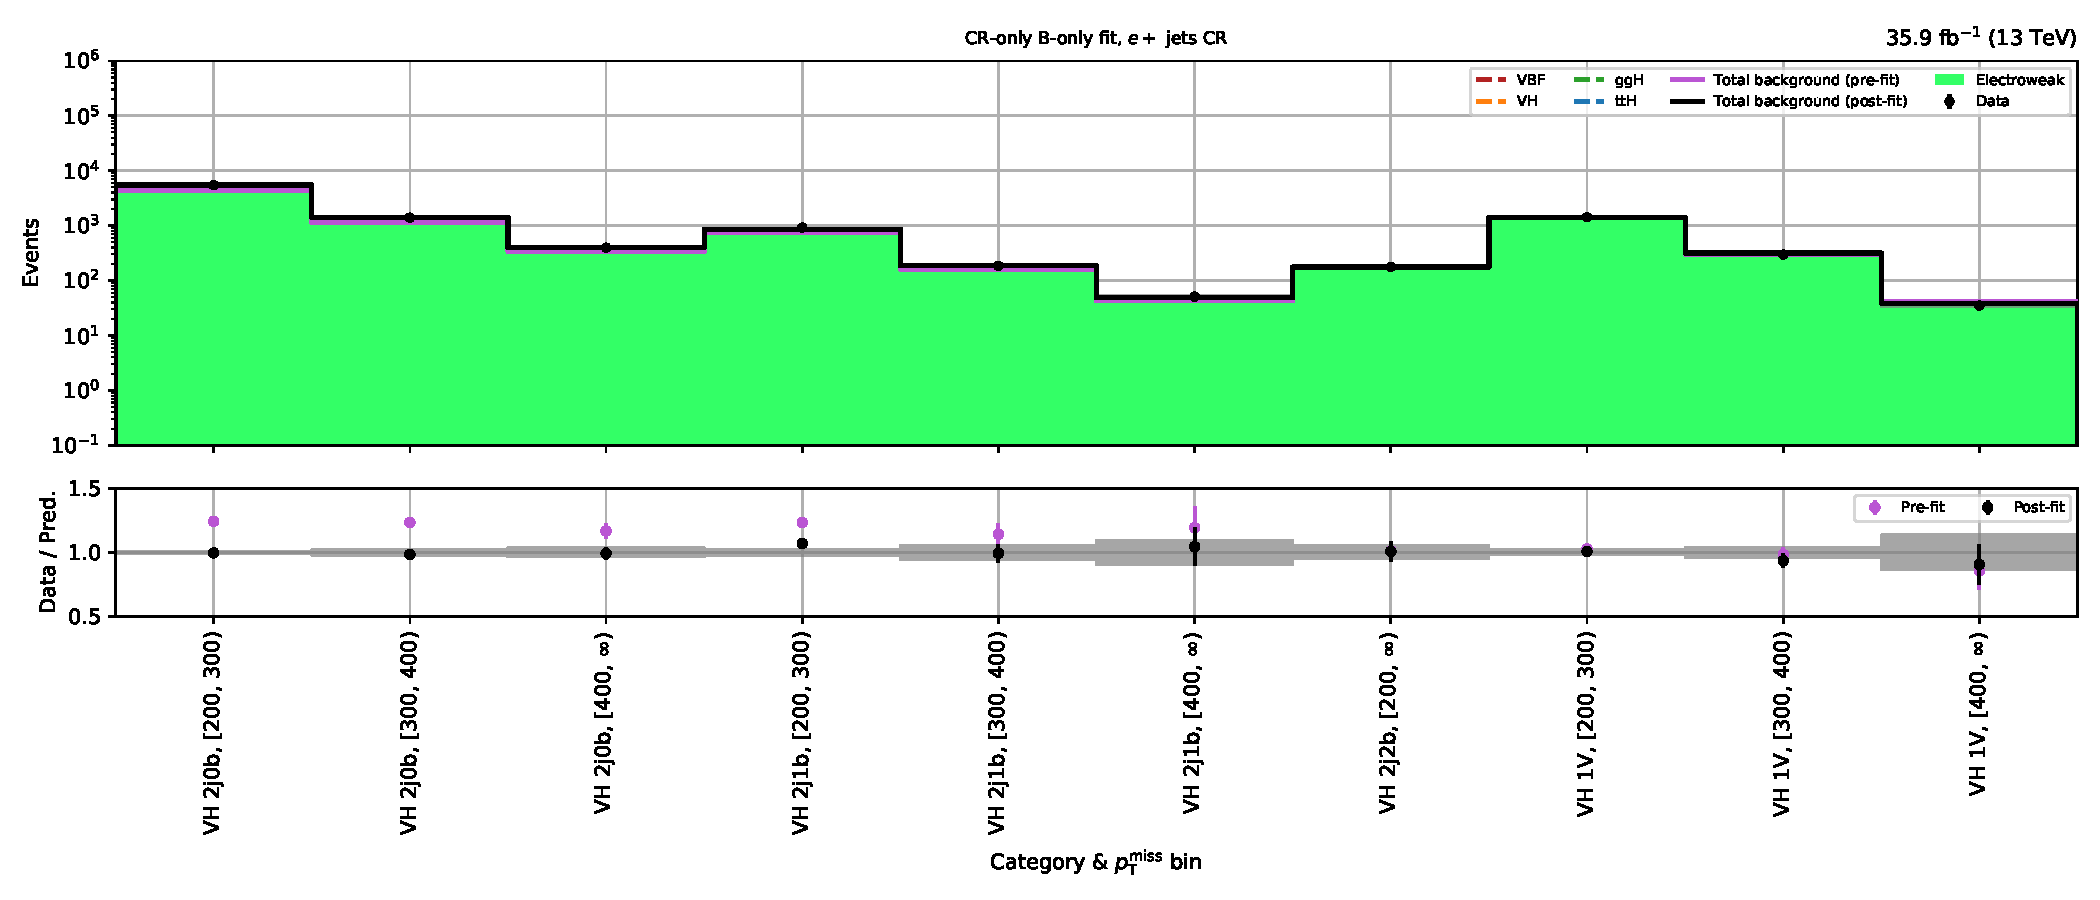
\includegraphics[width=\textwidth]{chapters/higgstoinv/figures/mountain_ranges/2016/VH/Wenu_tree_fit_b-abs_values_VH_cats.pdf}
        \caption{\VH --- \singleEleCr \gls{CR} (2016)}
    \end{subfigure}

    \begin{subfigure}[b]{0.49\textwidth}
        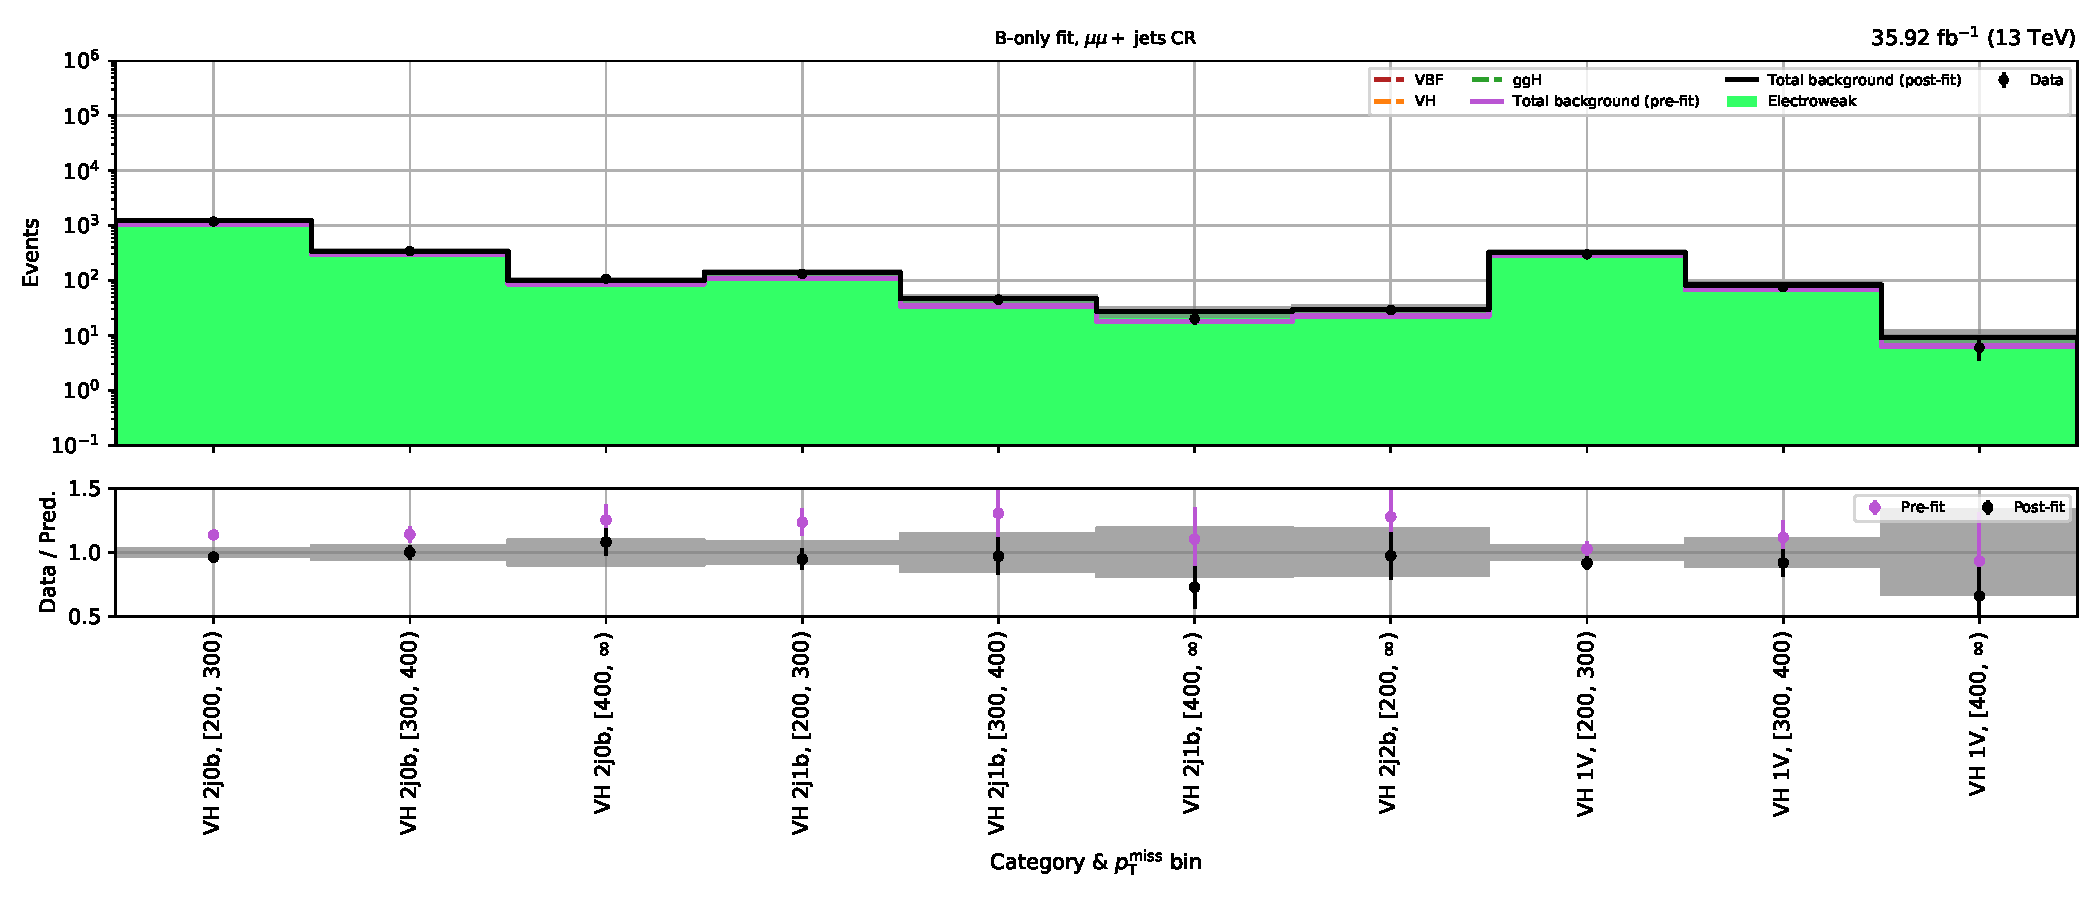
\includegraphics[width=\textwidth]{chapters/higgstoinv/figures/mountain_ranges/2016/VH/Zmumu_tree_fit_b-abs_values_VH_cats.pdf}
        \caption{\VH --- \doubleMuCr \gls{CR} (2016)}
    \end{subfigure}
    \hfill
    \begin{subfigure}[b]{0.49\textwidth}
        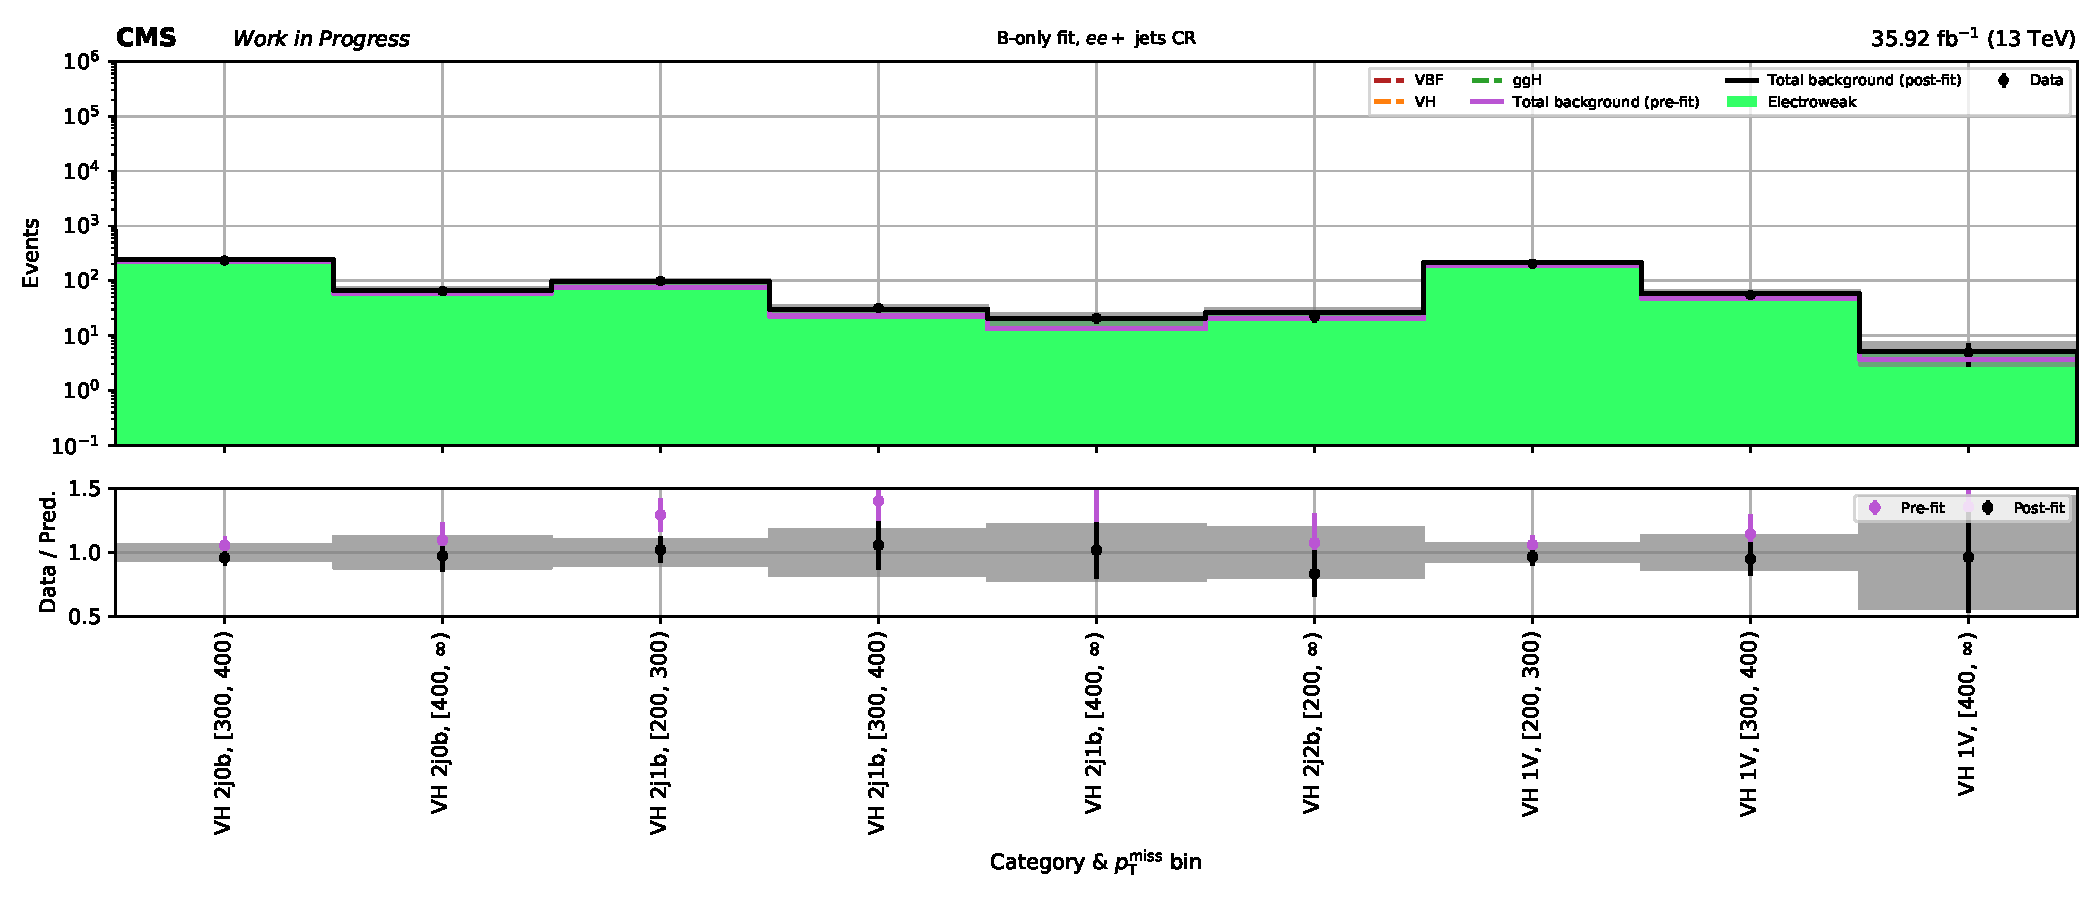
\includegraphics[width=\textwidth]{chapters/higgstoinv/figures/mountain_ranges/2016/VH/Zee_tree_fit_b-abs_values_VH_cats.pdf}
        \caption{\VH --- \doubleEleCr \gls{CR} (2016)}
    \end{subfigure}

    \begin{subfigure}[b]{0.49\textwidth}
        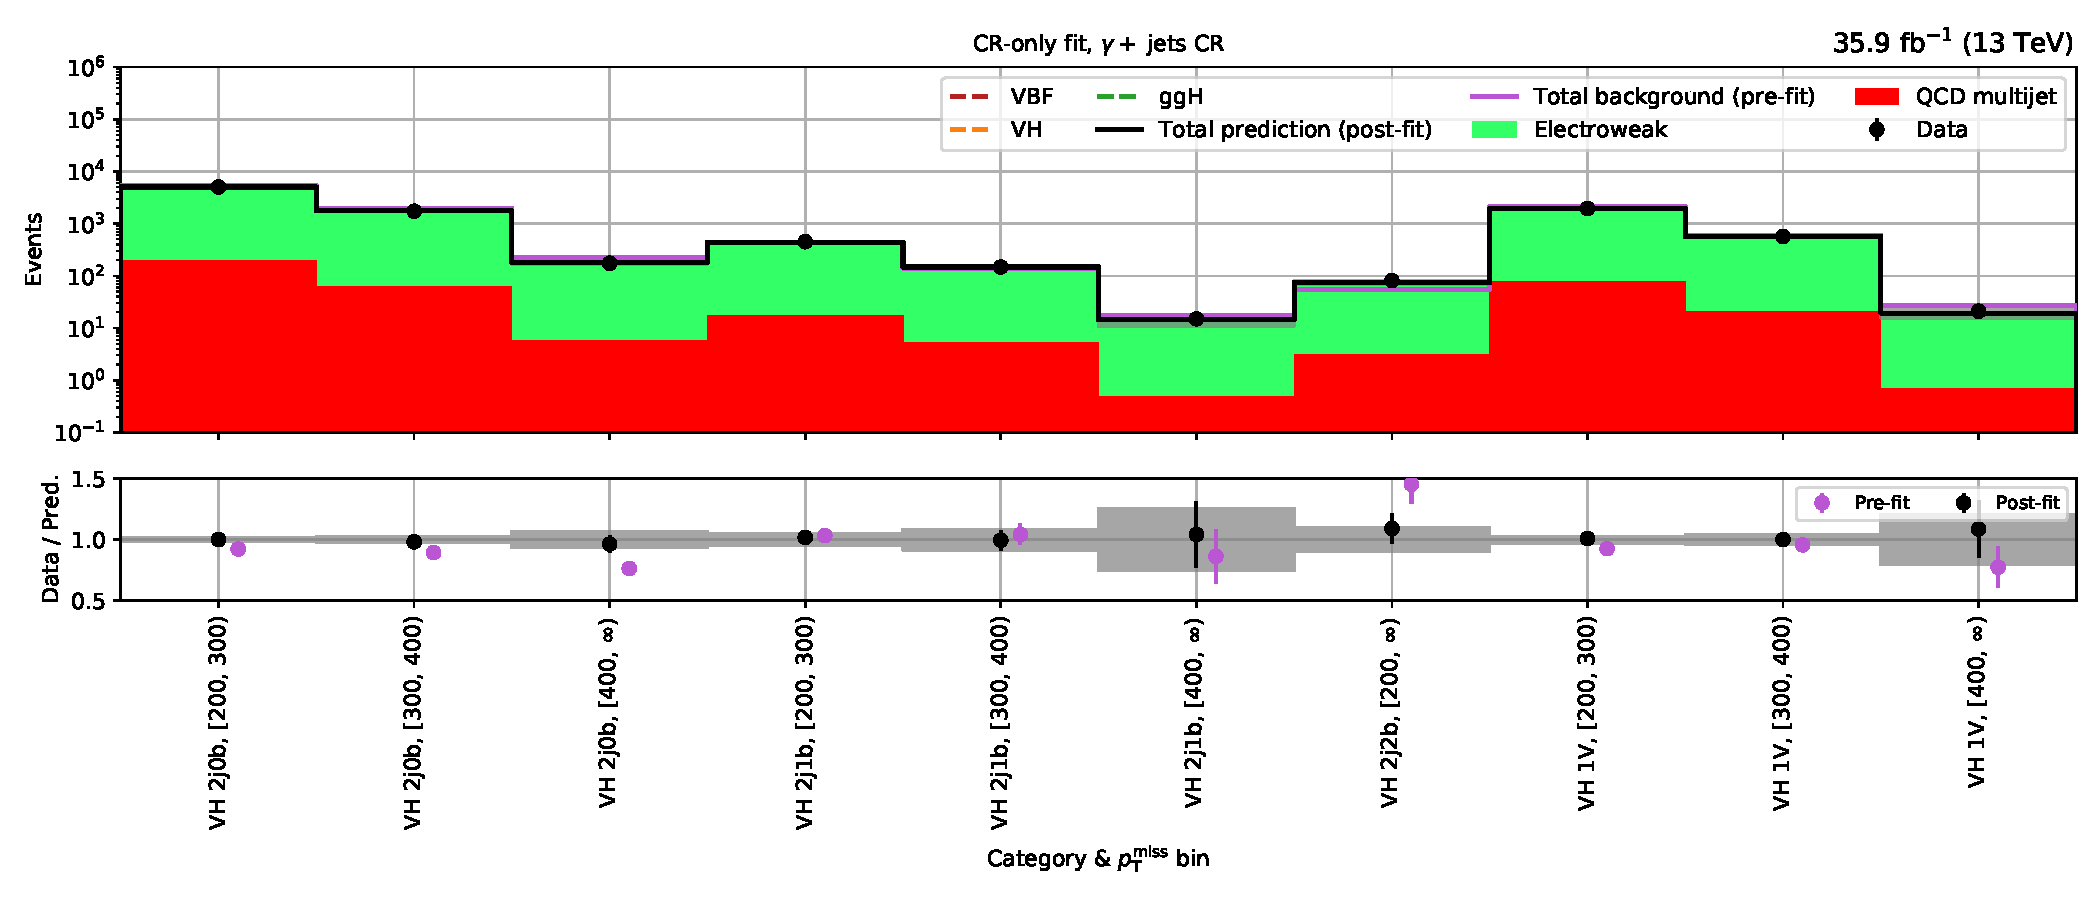
\includegraphics[width=\textwidth]{chapters/higgstoinv/figures/mountain_ranges/2016/VH/Photon_tree_fit_b-abs_values_VH_cats.pdf}
        \caption{\VH --- \singlePhotonCr \gls{CR} (2016)}
    \end{subfigure}
    \caption[Post-fit yields for each \VH subcategory and \ptmiss bin in the lepton and photon control regions for the 2016 dataset]{Post-fit yields for each \VH subcategory and \ptmiss bin in the lepton and photon \glspl{CR} for the 2016 dataset. The total background pre-fit and post-fit is compared to data in the lower panel of each subfigure.}
    \label{fig:htoinv_mountain_range_VH_2016_CRs}
\end{figure}

\begin{figure}[htbp]
    \centering
    \begin{subfigure}[b]{0.49\textwidth}
        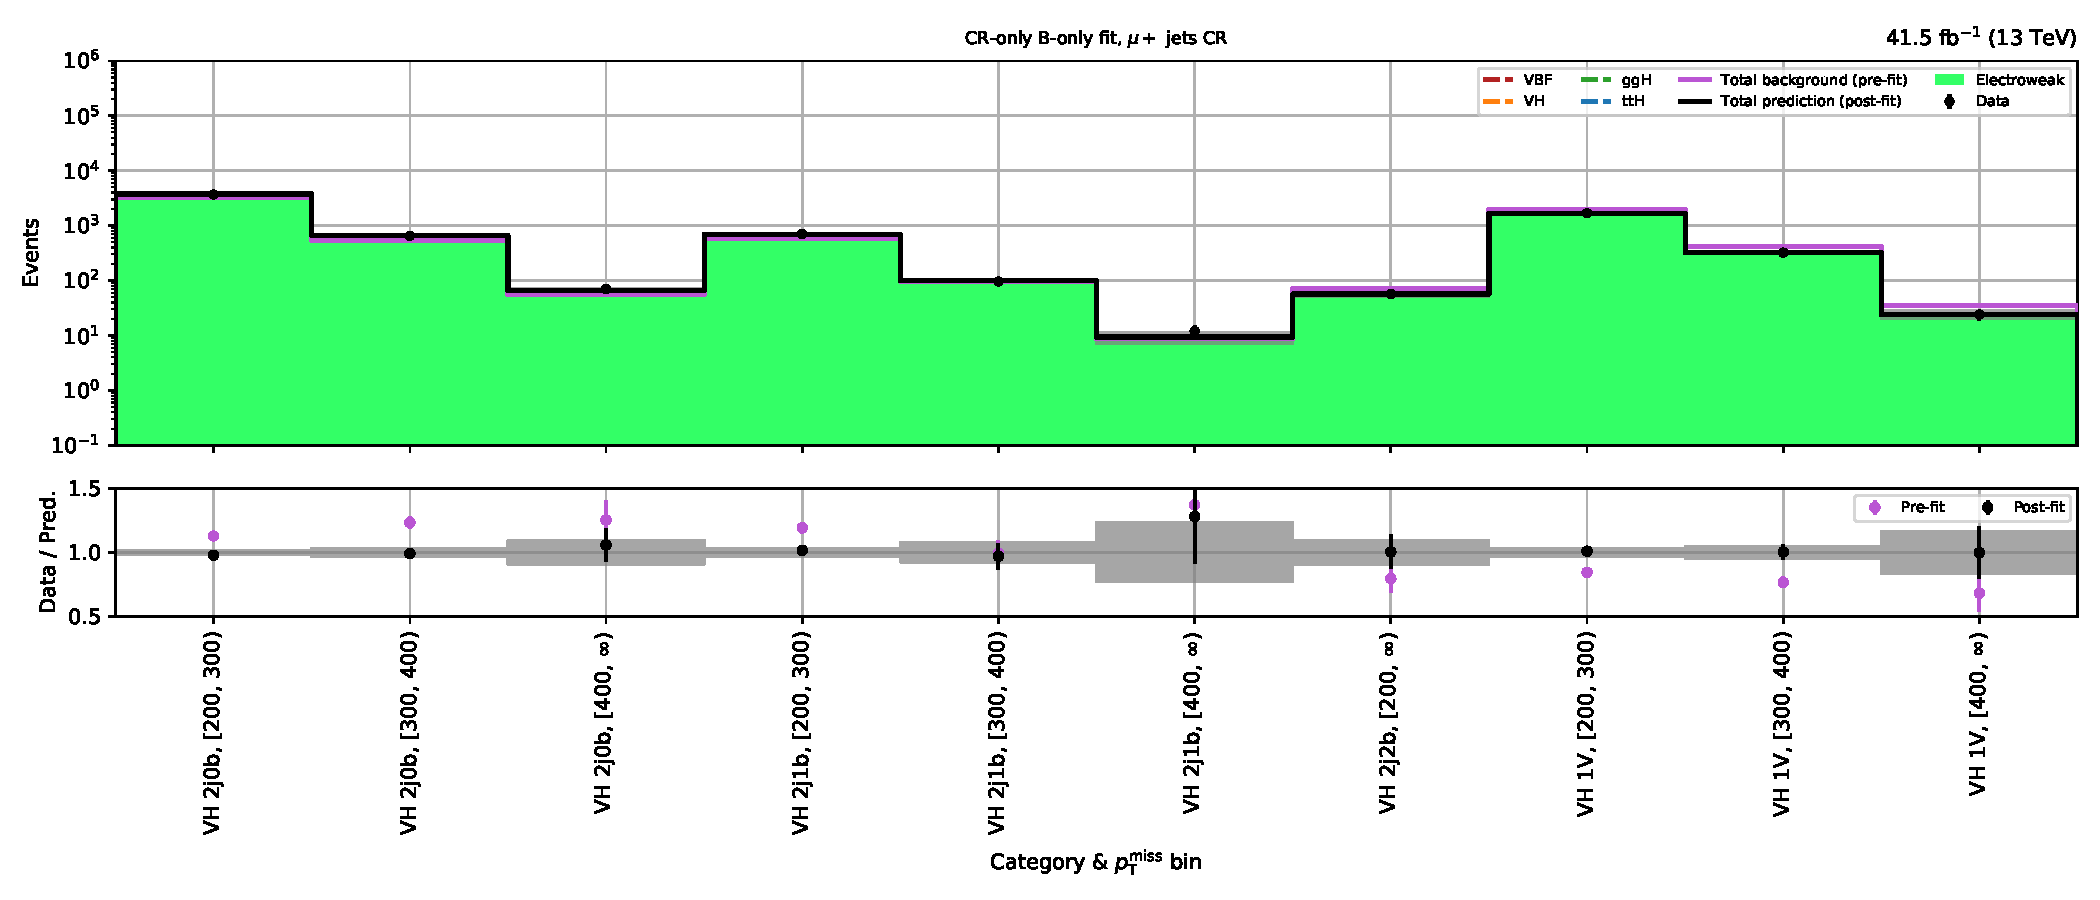
\includegraphics[width=\textwidth]{chapters/higgstoinv/figures/mountain_ranges/2017/VH/Wmunu_tree_fit_b-abs_values_VH_cats.pdf}
        \caption{\VH --- \singleMuCr \gls{CR} (2017)}
    \end{subfigure}
    \hfill
    \begin{subfigure}[b]{0.49\textwidth}
        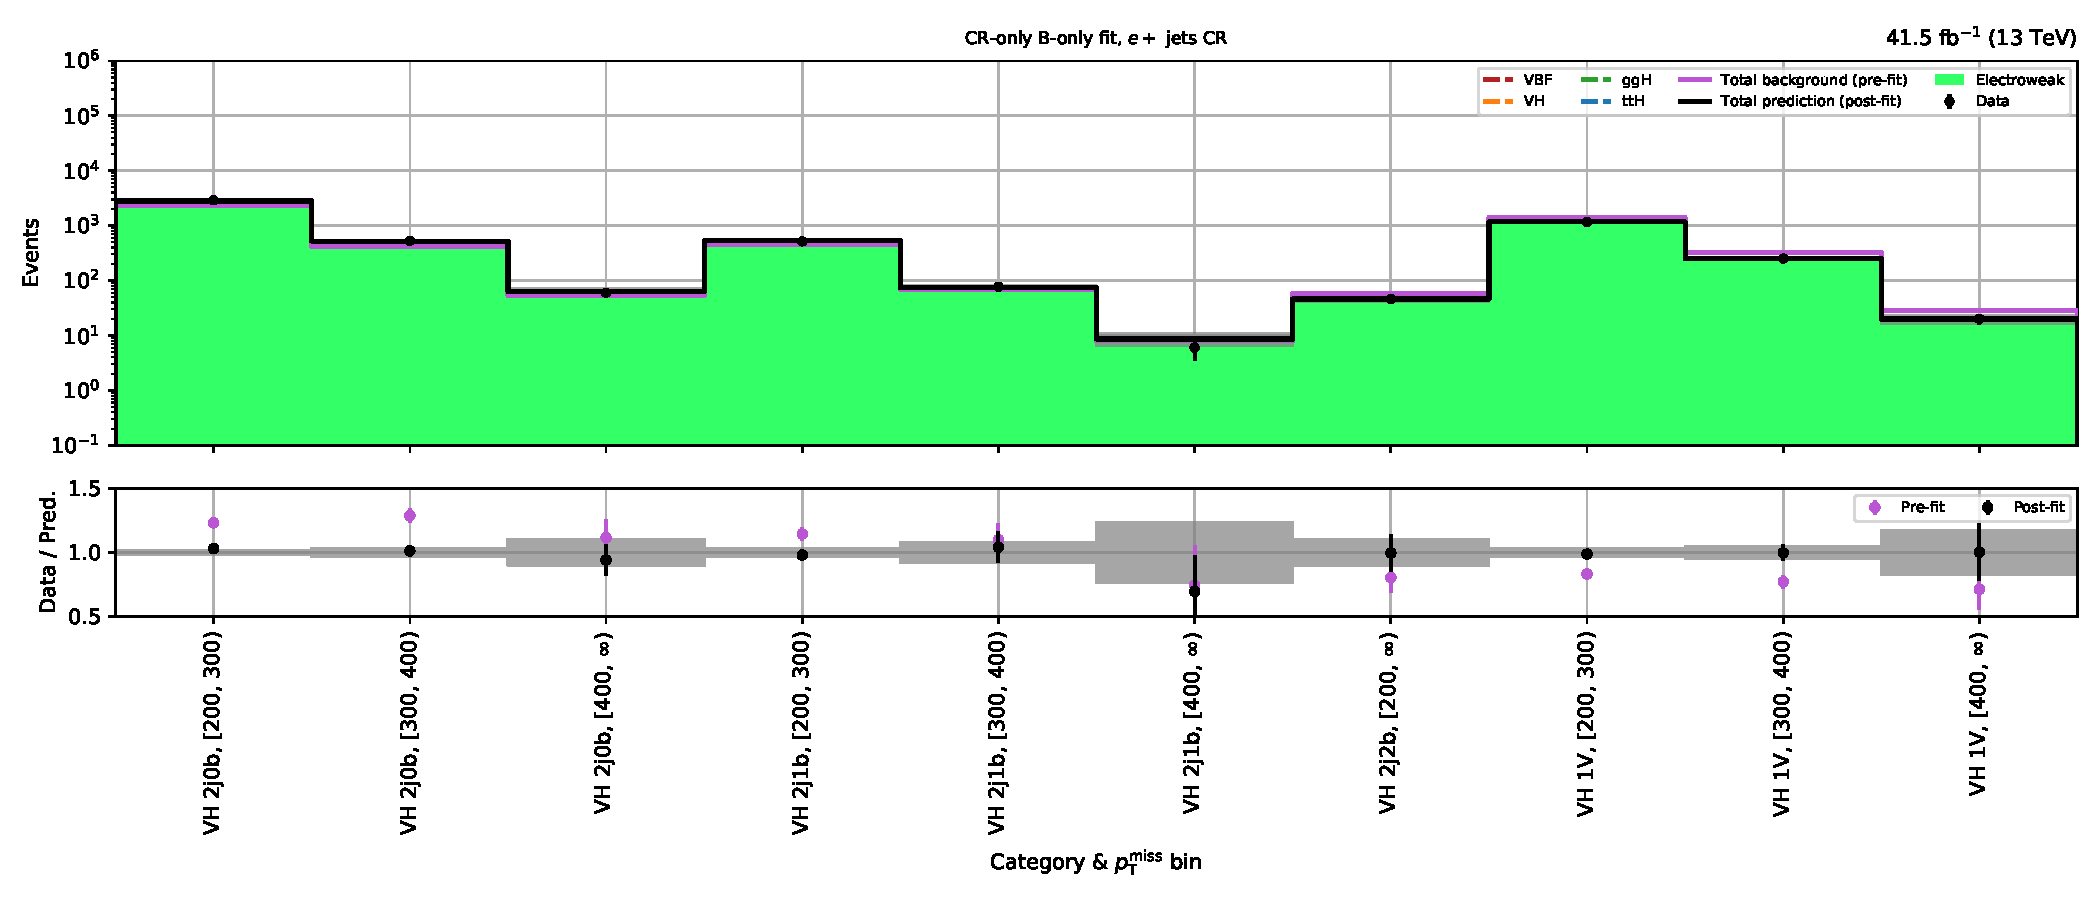
\includegraphics[width=\textwidth]{chapters/higgstoinv/figures/mountain_ranges/2017/VH/Wenu_tree_fit_b-abs_values_VH_cats.pdf}
        \caption{\VH --- \singleEleCr \gls{CR} (2017)}
    \end{subfigure}

    \begin{subfigure}[b]{0.49\textwidth}
        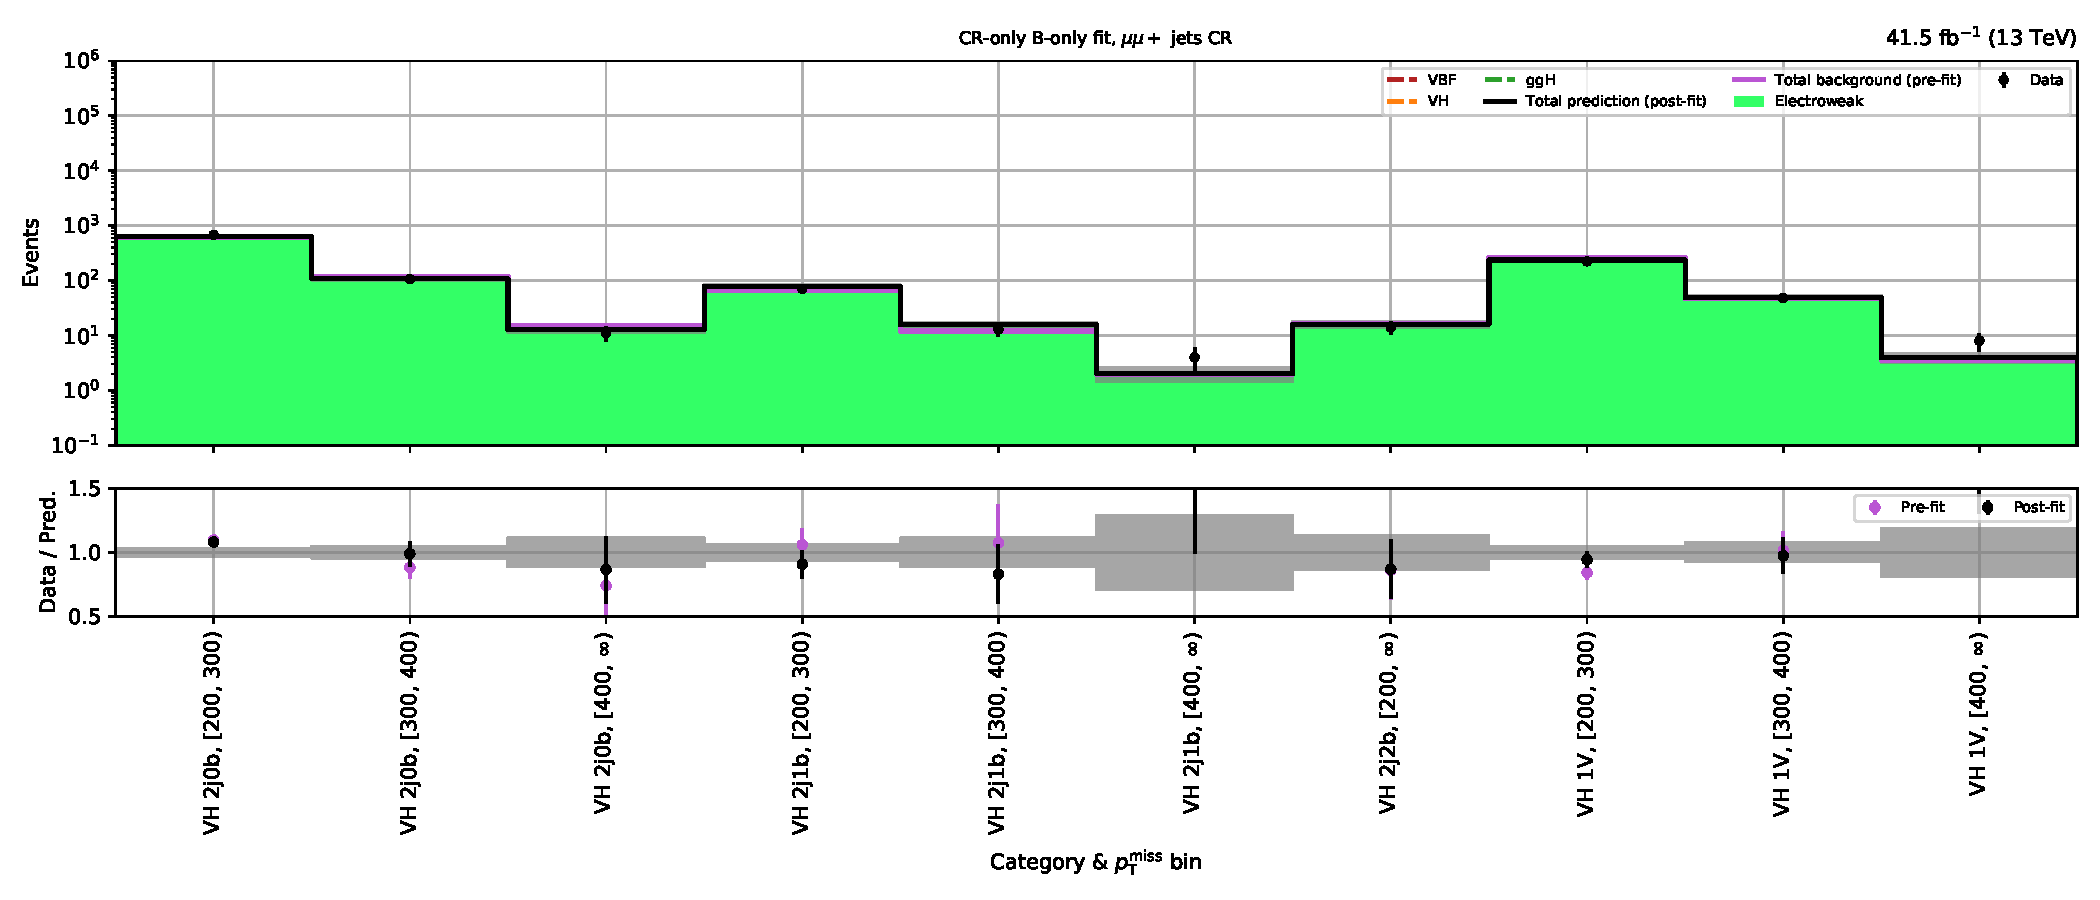
\includegraphics[width=\textwidth]{chapters/higgstoinv/figures/mountain_ranges/2017/VH/Zmumu_tree_fit_b-abs_values_VH_cats.pdf}
        \caption{\VH --- \doubleMuCr \gls{CR} (2017)}
    \end{subfigure}
    \hfill
    \begin{subfigure}[b]{0.49\textwidth}
        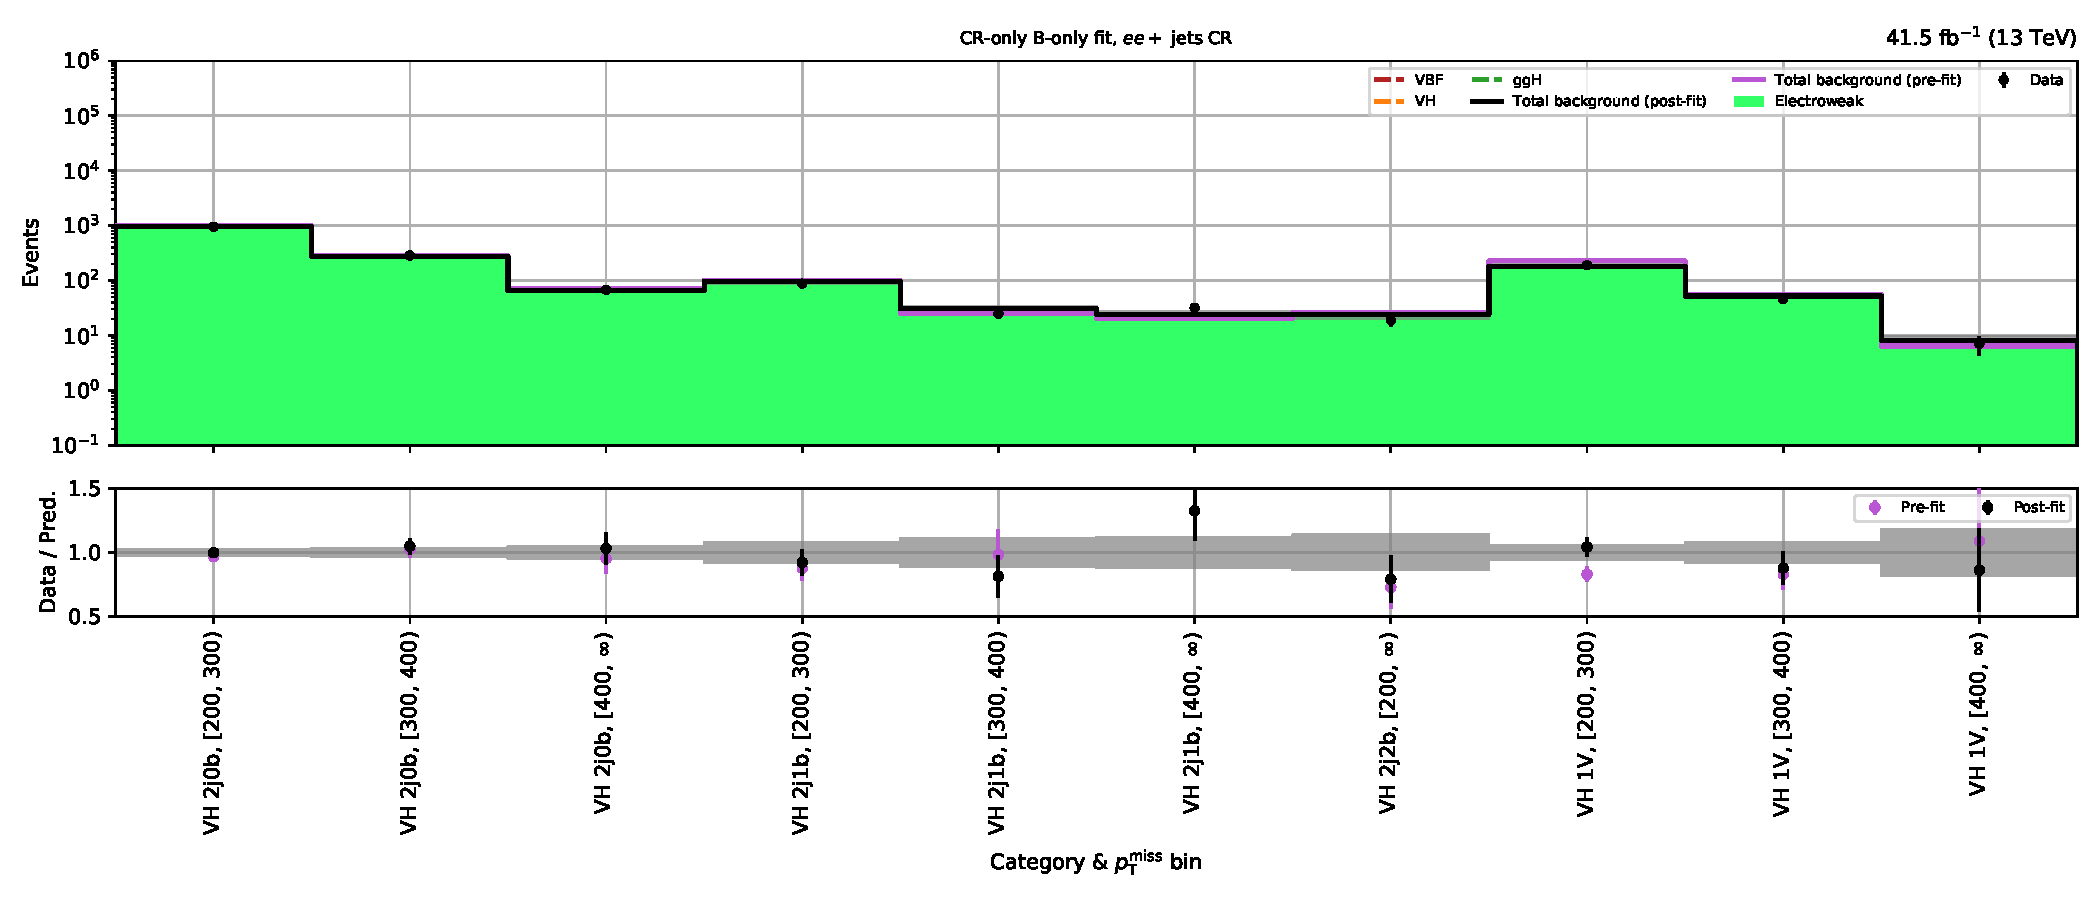
\includegraphics[width=\textwidth]{chapters/higgstoinv/figures/mountain_ranges/2017/VH/Zee_tree_fit_b-abs_values_VH_cats.pdf}
        \caption{\VH --- \doubleEleCr \gls{CR} (2017)}
    \end{subfigure}

    \begin{subfigure}[b]{0.49\textwidth}
        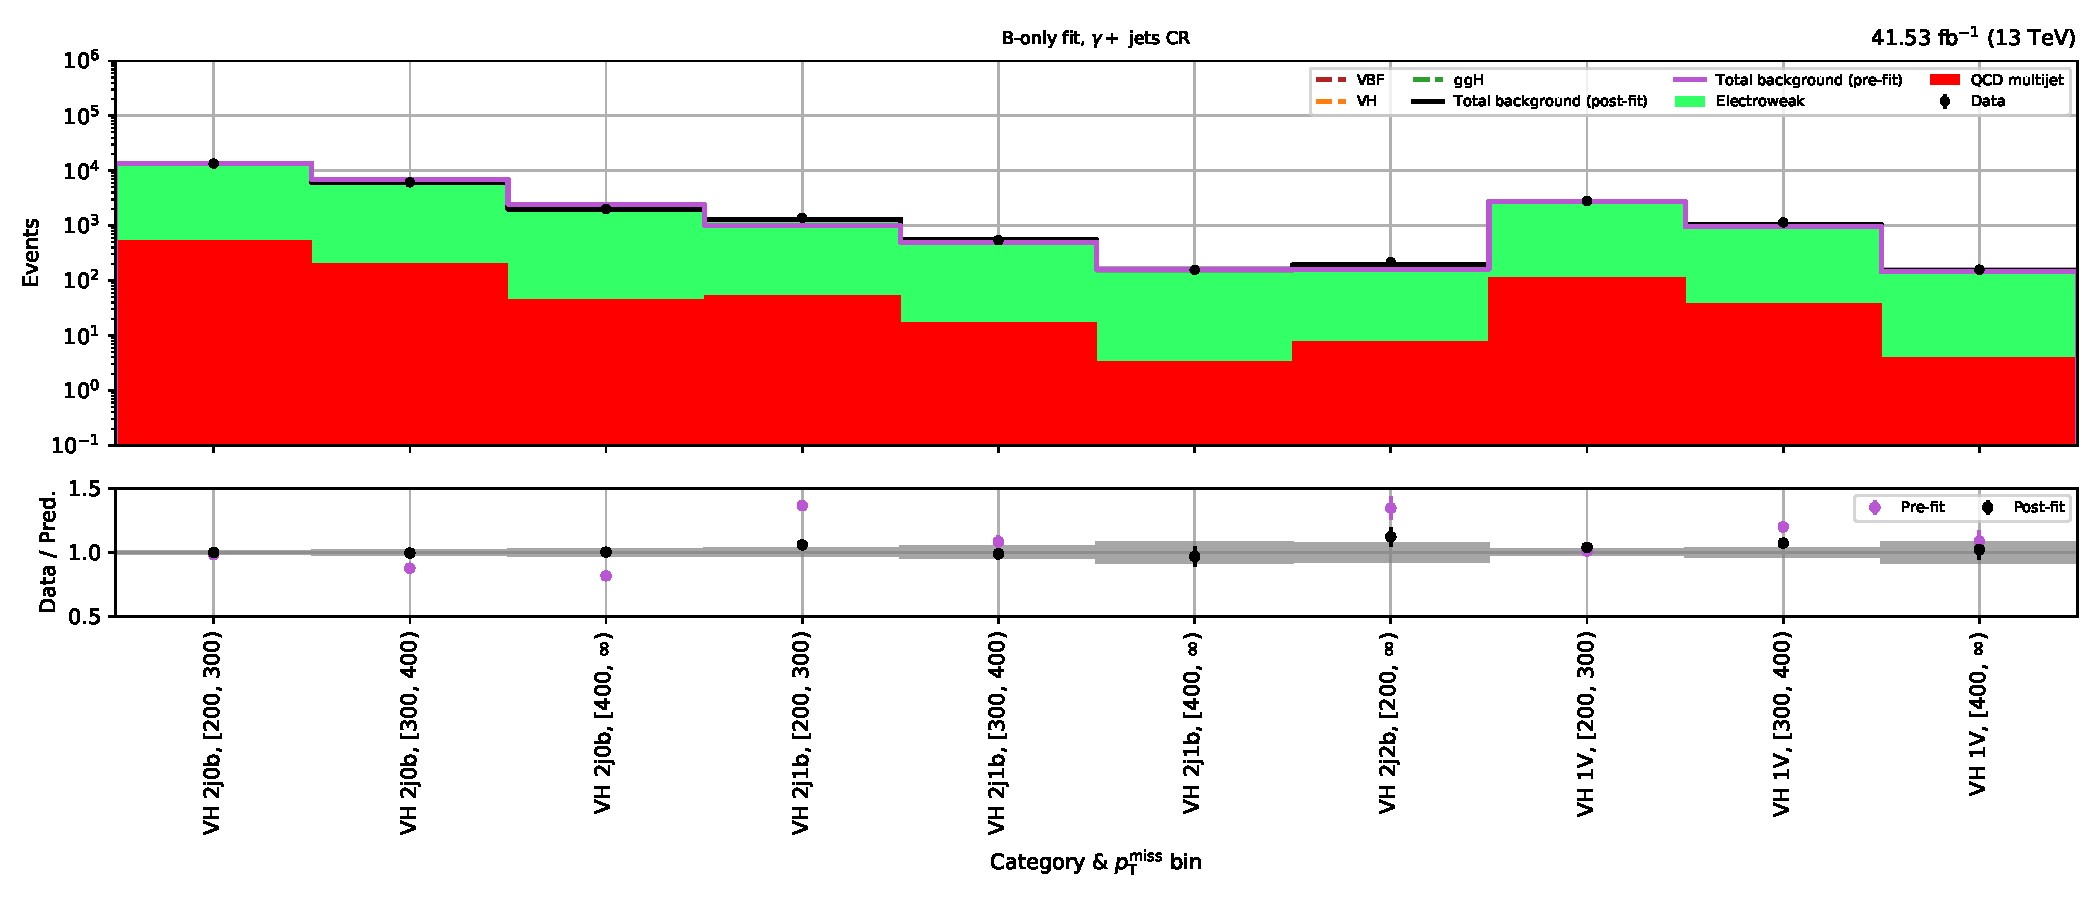
\includegraphics[width=\textwidth]{chapters/higgstoinv/figures/mountain_ranges/2017/VH/Photon_tree_fit_b-abs_values_VH_cats.pdf}
        \caption{\VH --- \singlePhotonCr \gls{CR} (2017)}
    \end{subfigure}
    \caption[Post-fit yields for each \VH subcategory and \ptmiss bin in the lepton and photon control regions for the 2017 dataset]{Post-fit yields for each \VH subcategory and \ptmiss bin in the lepton and photon \glspl{CR} for the 2017 dataset. The total background pre-fit and post-fit is compared to data in the lower panel of each subfigure.}
    \label{fig:htoinv_mountain_range_VH_2017_CRs}
\end{figure}

\begin{figure}[htbp]
    \centering
    \begin{subfigure}[b]{0.49\textwidth}
        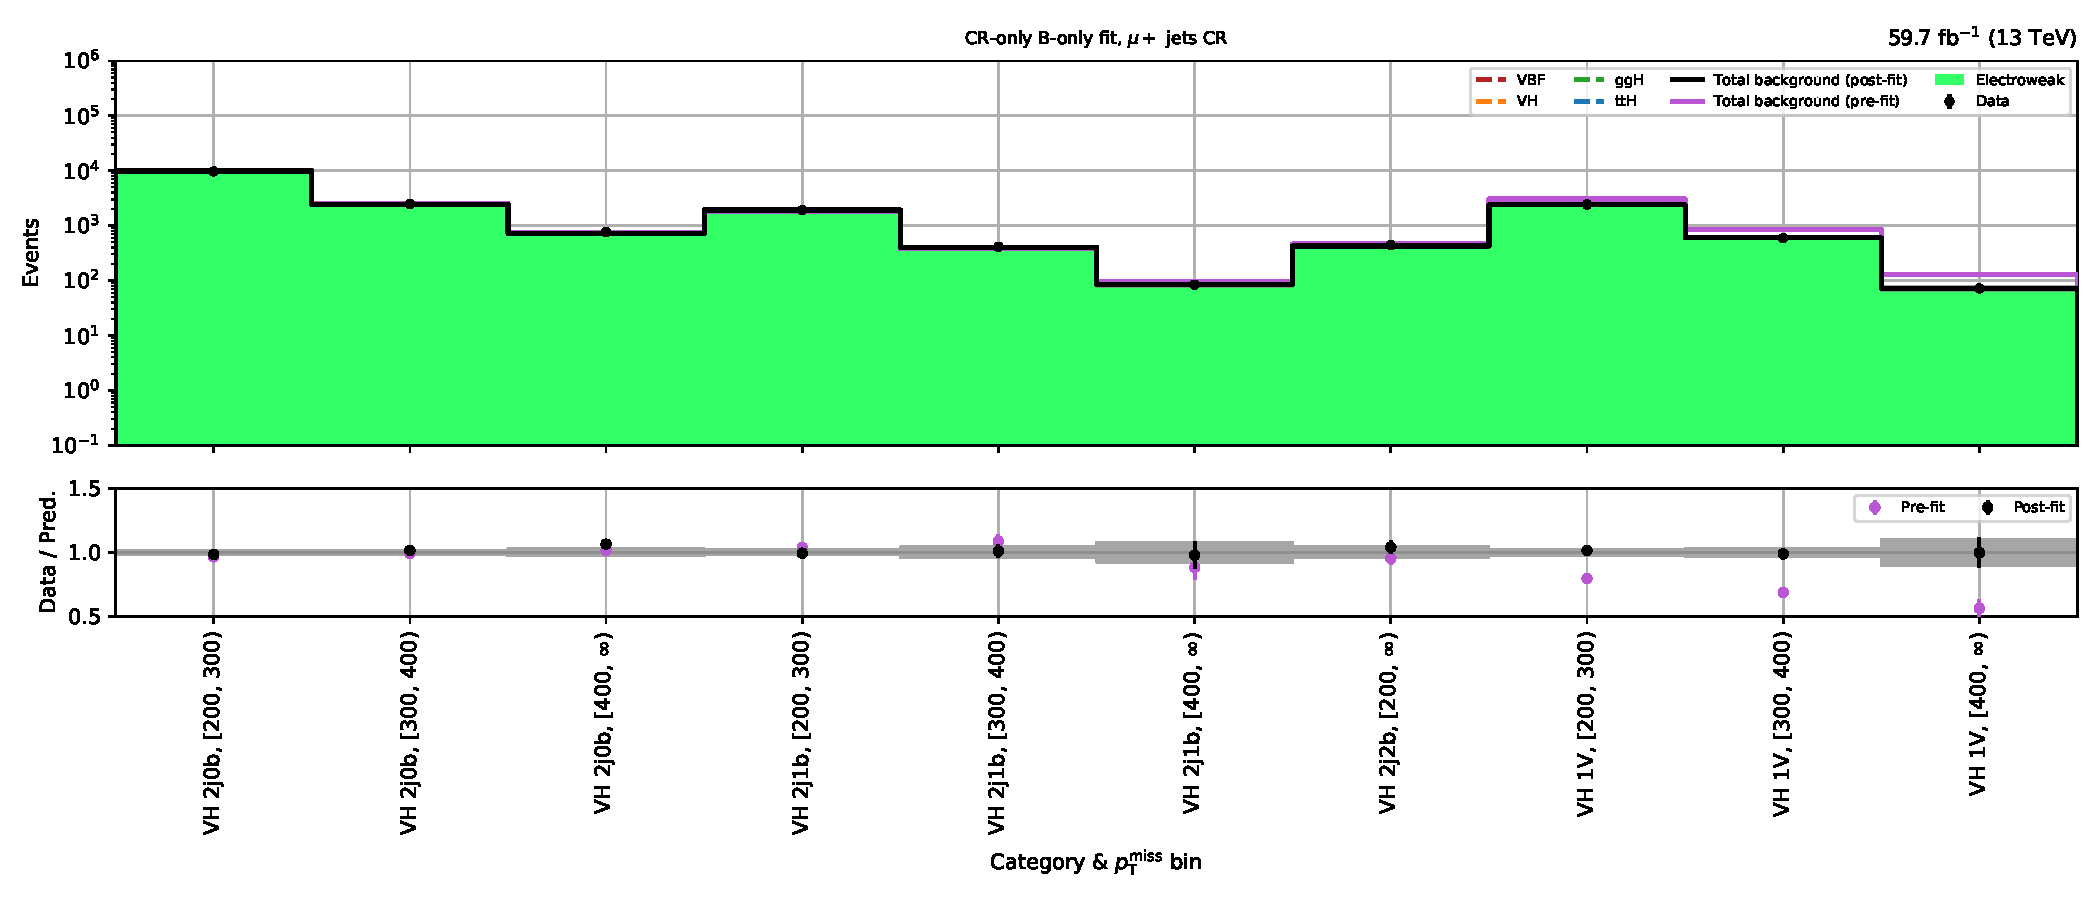
\includegraphics[width=\textwidth]{chapters/higgstoinv/figures/mountain_ranges/2018/VH/Wmunu_tree_fit_b-abs_values_VH_cats.pdf}
        \caption{\VH --- \singleMuCr \gls{CR} (2018)}
    \end{subfigure}
    \hfill
    \begin{subfigure}[b]{0.49\textwidth}
        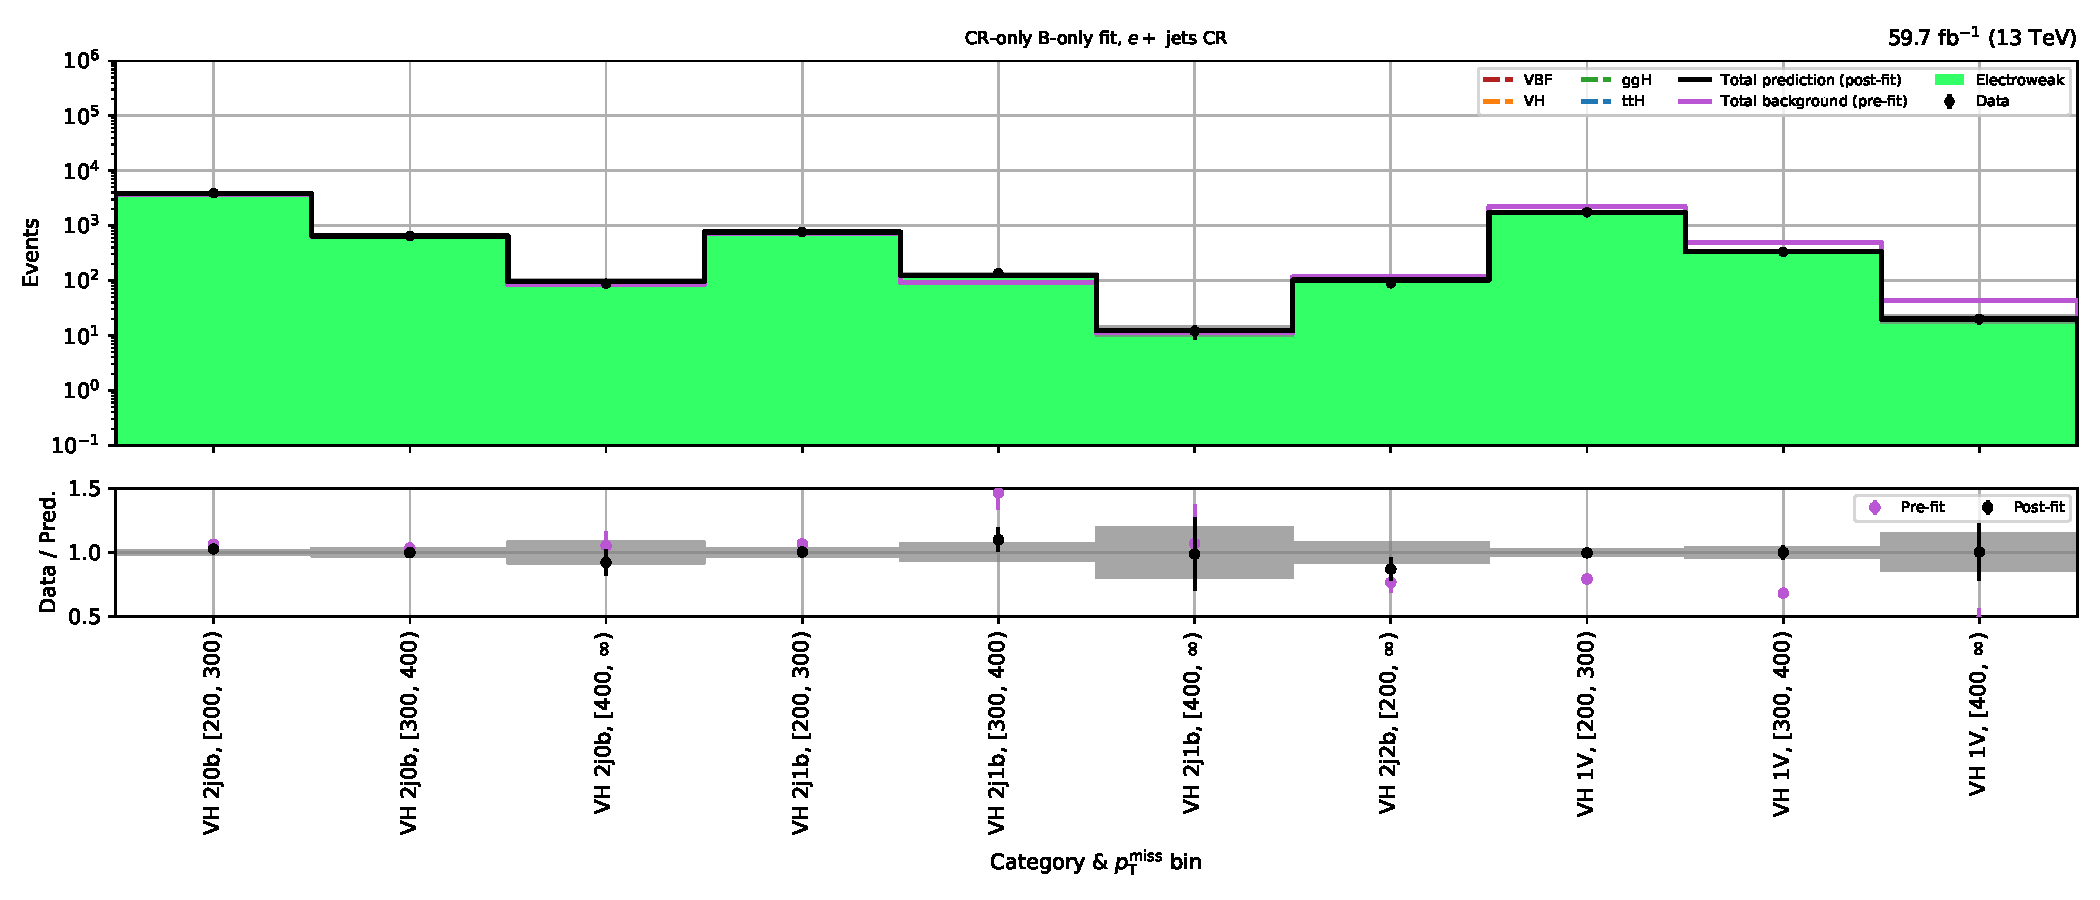
\includegraphics[width=\textwidth]{chapters/higgstoinv/figures/mountain_ranges/2018/VH/Wenu_tree_fit_b-abs_values_VH_cats.pdf}
        \caption{\VH --- \singleEleCr \gls{CR} (2018)}
    \end{subfigure}

    \begin{subfigure}[b]{0.49\textwidth}
        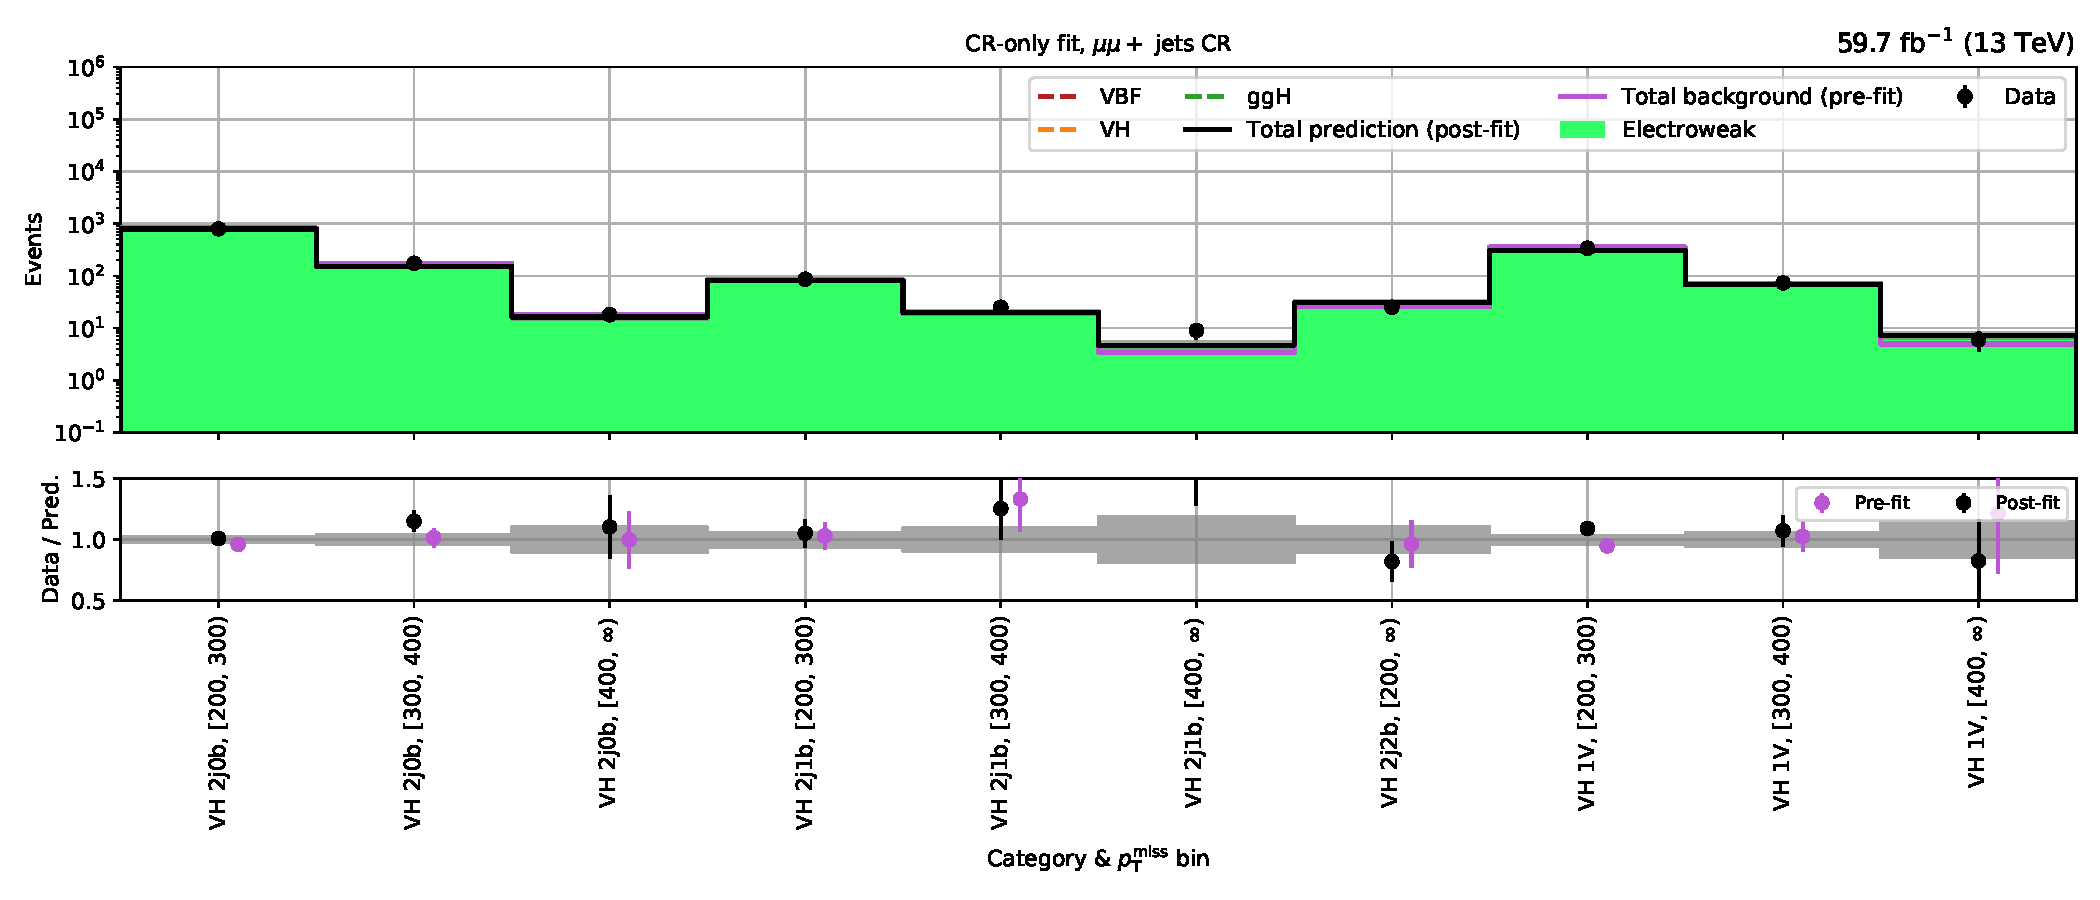
\includegraphics[width=\textwidth]{chapters/higgstoinv/figures/mountain_ranges/2018/VH/Zmumu_tree_fit_b-abs_values_VH_cats.pdf}
        \caption{\VH --- \doubleMuCr \gls{CR} (2018)}
    \end{subfigure}
    \hfill
    \begin{subfigure}[b]{0.49\textwidth}
        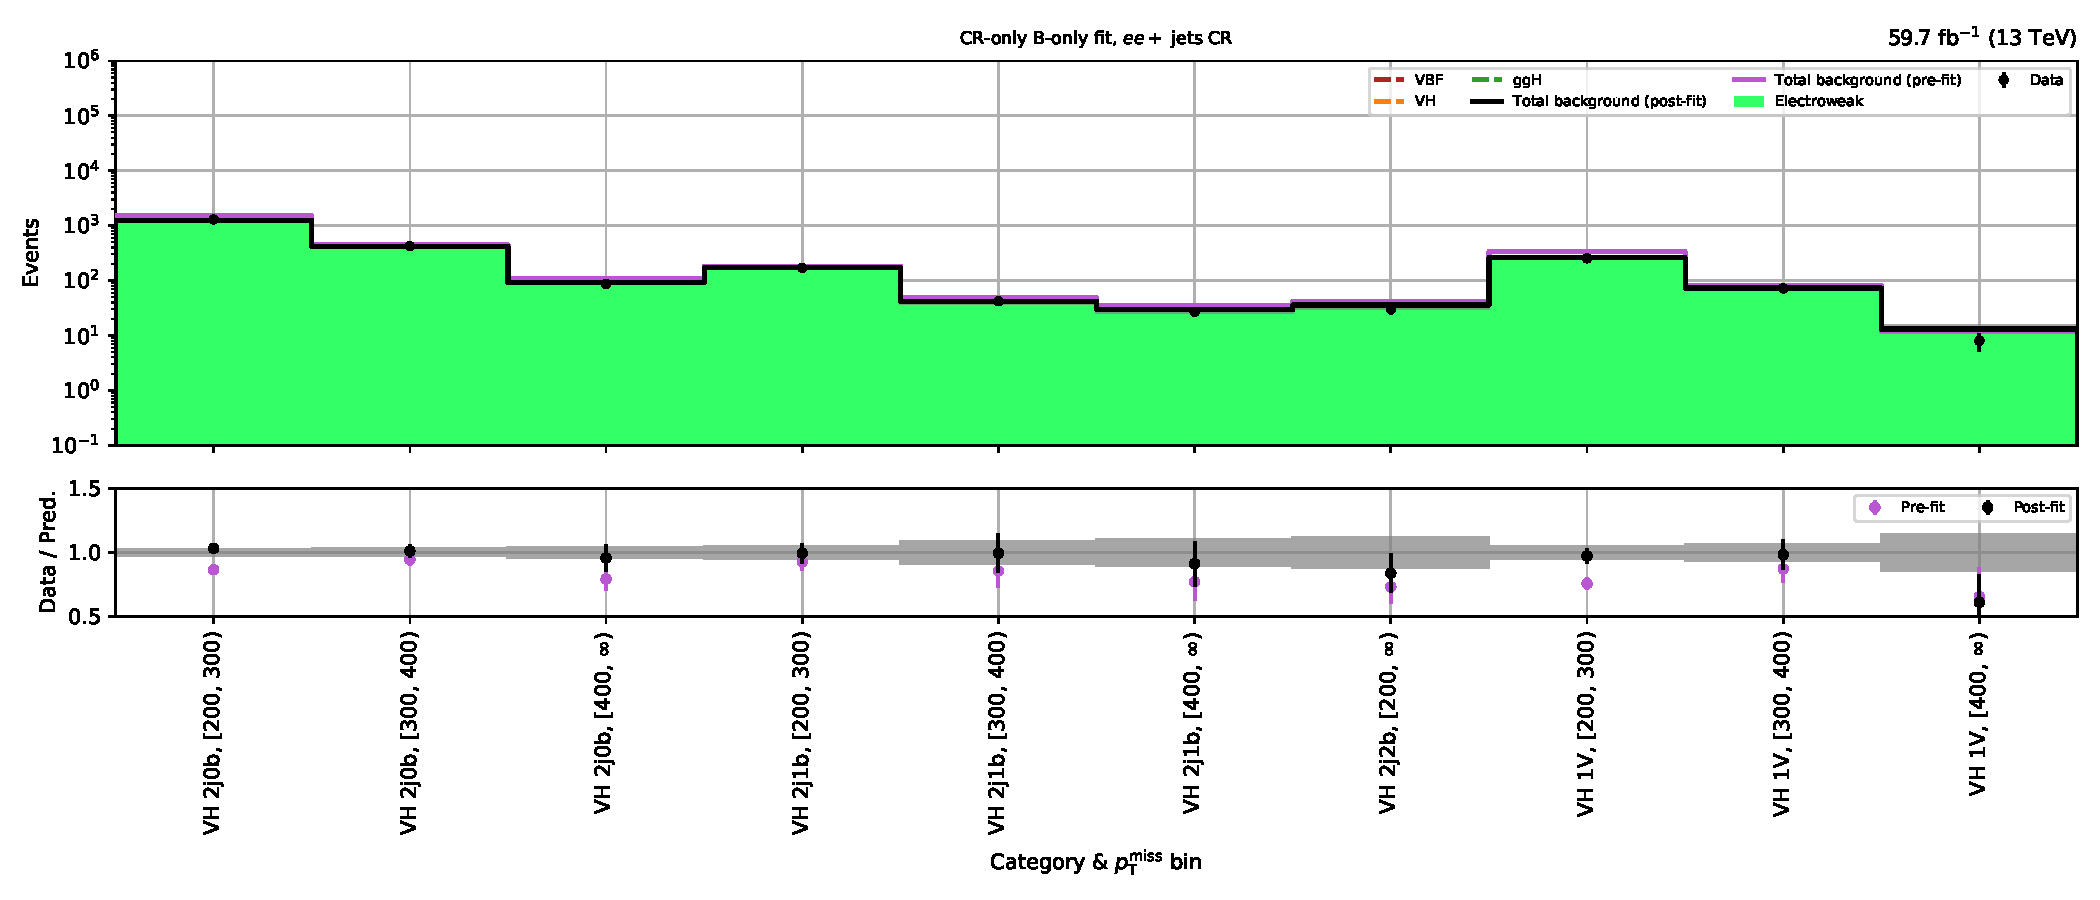
\includegraphics[width=\textwidth]{chapters/higgstoinv/figures/mountain_ranges/2018/VH/Zee_tree_fit_b-abs_values_VH_cats.pdf}
        \caption{\VH --- \doubleEleCr \gls{CR} (2018)}
    \end{subfigure}

    \begin{subfigure}[b]{0.49\textwidth}
        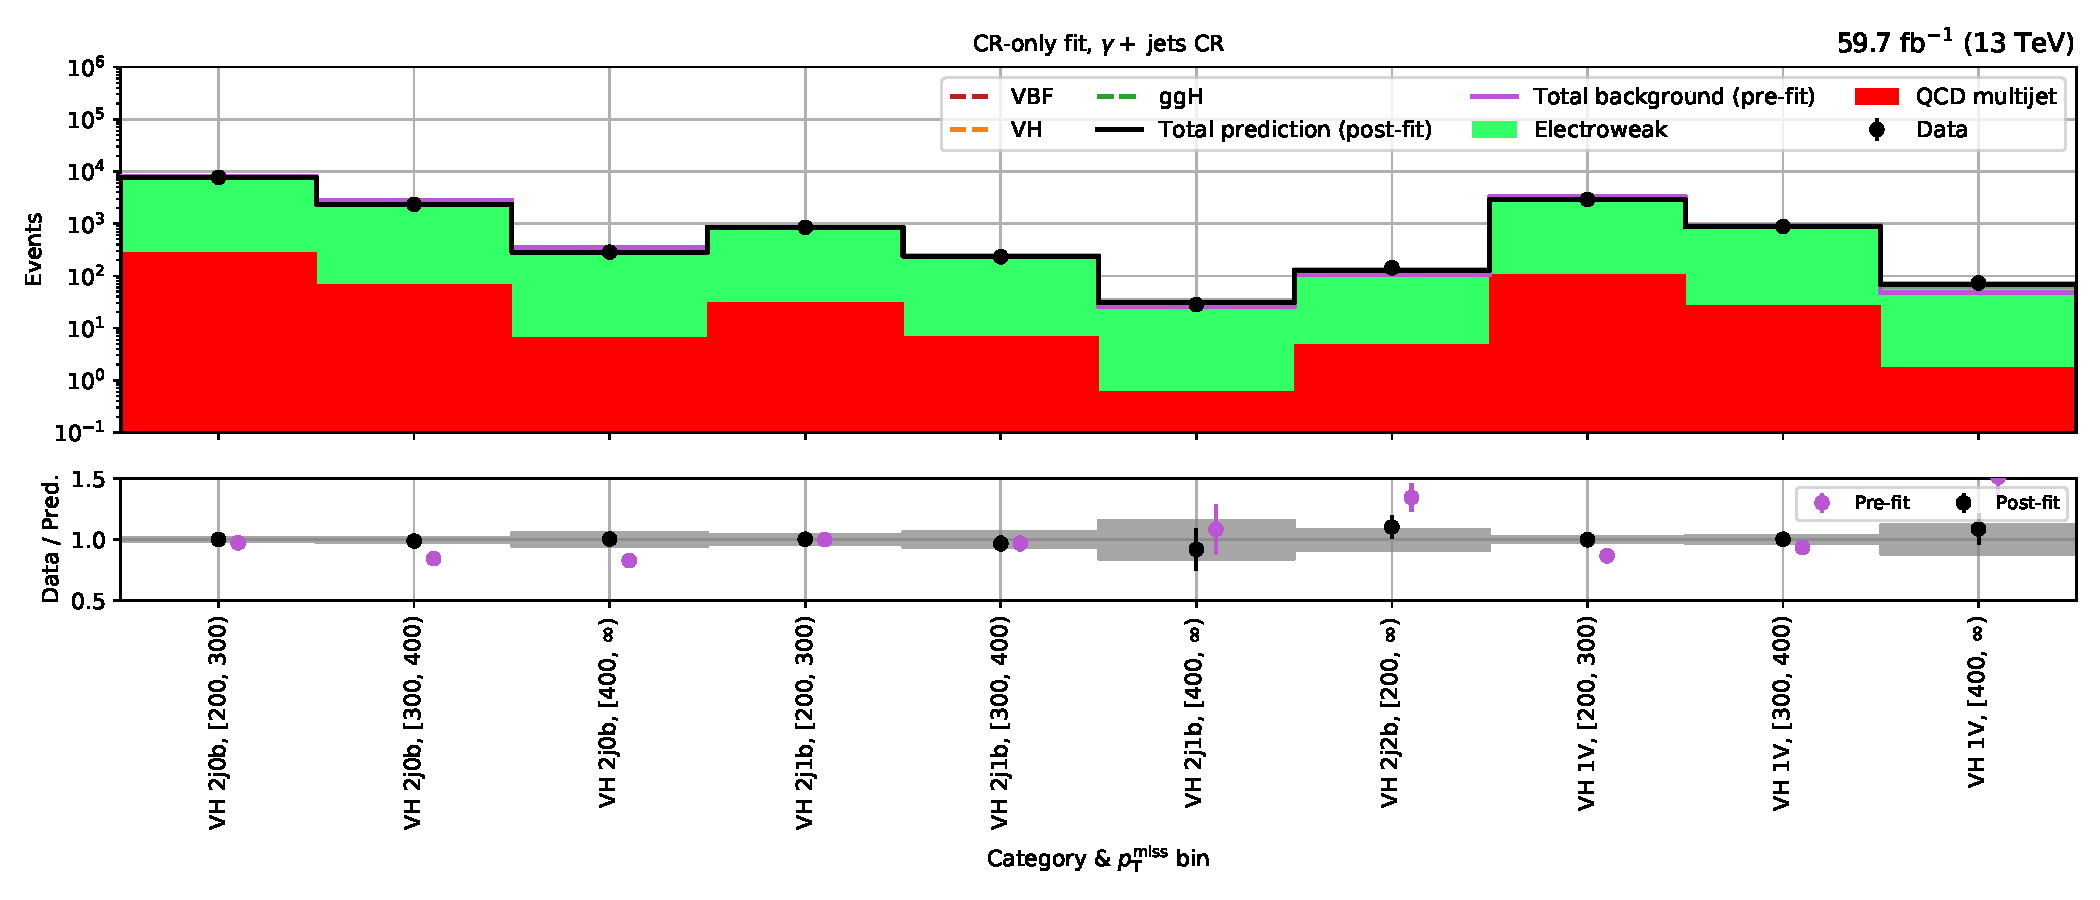
\includegraphics[width=\textwidth]{chapters/higgstoinv/figures/mountain_ranges/2018/VH/Photon_tree_fit_b-abs_values_VH_cats.pdf}
        \caption{\VH --- \singlePhotonCr \gls{CR} (2018)}
    \end{subfigure}
    \caption[Post-fit yields for each \VH subcategory and \ptmiss bin in the lepton and photon control regions for the 2018 dataset]{Post-fit yields for each \VH subcategory and \ptmiss bin in the lepton and photon \glspl{CR} for the 2018 dataset. The total background pre-fit and post-fit is compared to data in the lower panel of each subfigure.}
    \label{fig:htoinv_mountain_range_VH_2018_CRs}
\end{figure}

\clearpage


%=========================================================

\section{Limits and likelihood scans for each category}
\label{sec:limits_likelihoods_cats_supplementary}

\begin{figure}[htbp]
    \centering
    \begin{subfigure}[b]{0.45\textwidth}
        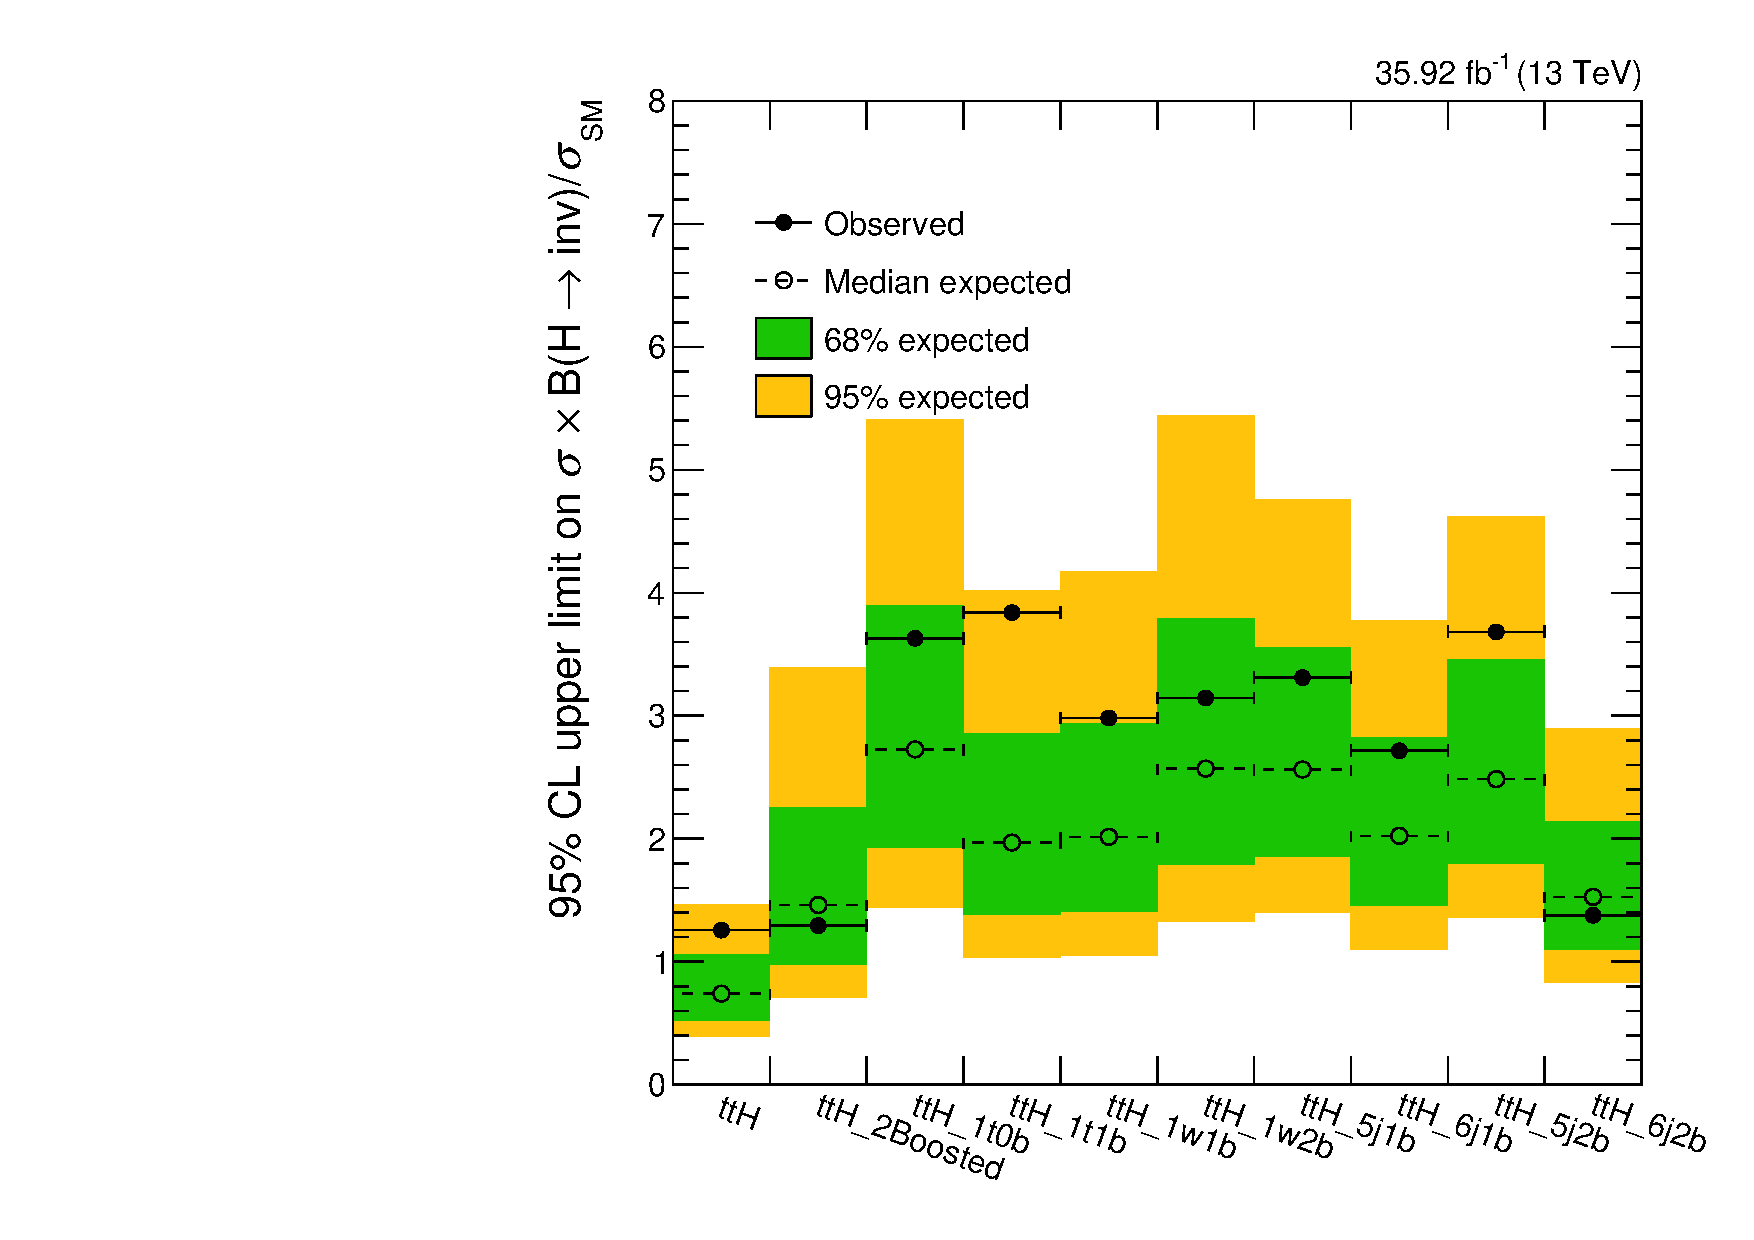
\includegraphics[width=\textwidth]{chapters/higgstoinv/figures/limits/ttH/limit_2016_ttH.pdf}
        \caption{\ttH --- 2016}
    \end{subfigure}
    \hfill
    \begin{subfigure}[b]{0.45\textwidth}
        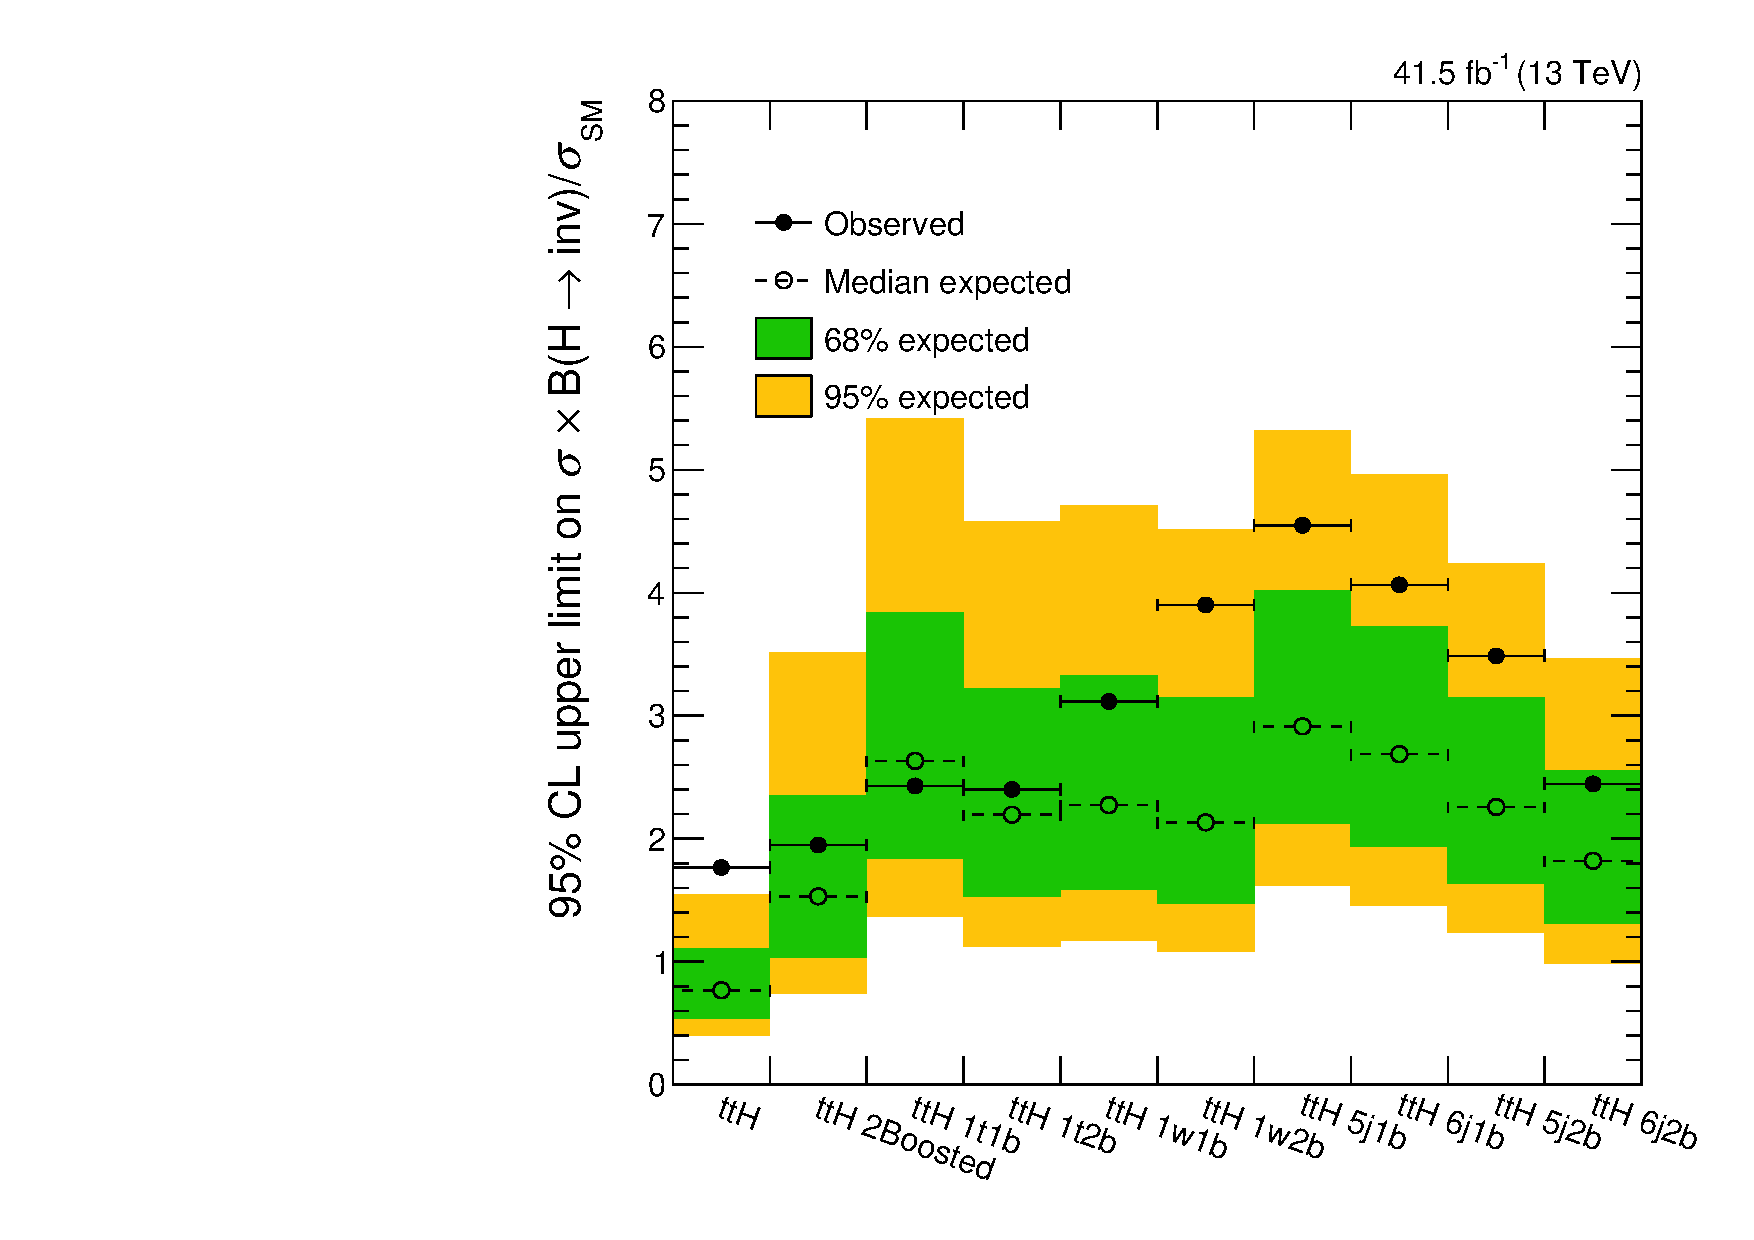
\includegraphics[width=\textwidth]{chapters/higgstoinv/figures/limits/ttH/limit_2017_ttH.pdf}
        \caption{\ttH --- 2017}
    \end{subfigure}

    \begin{subfigure}[b]{0.45\textwidth}
        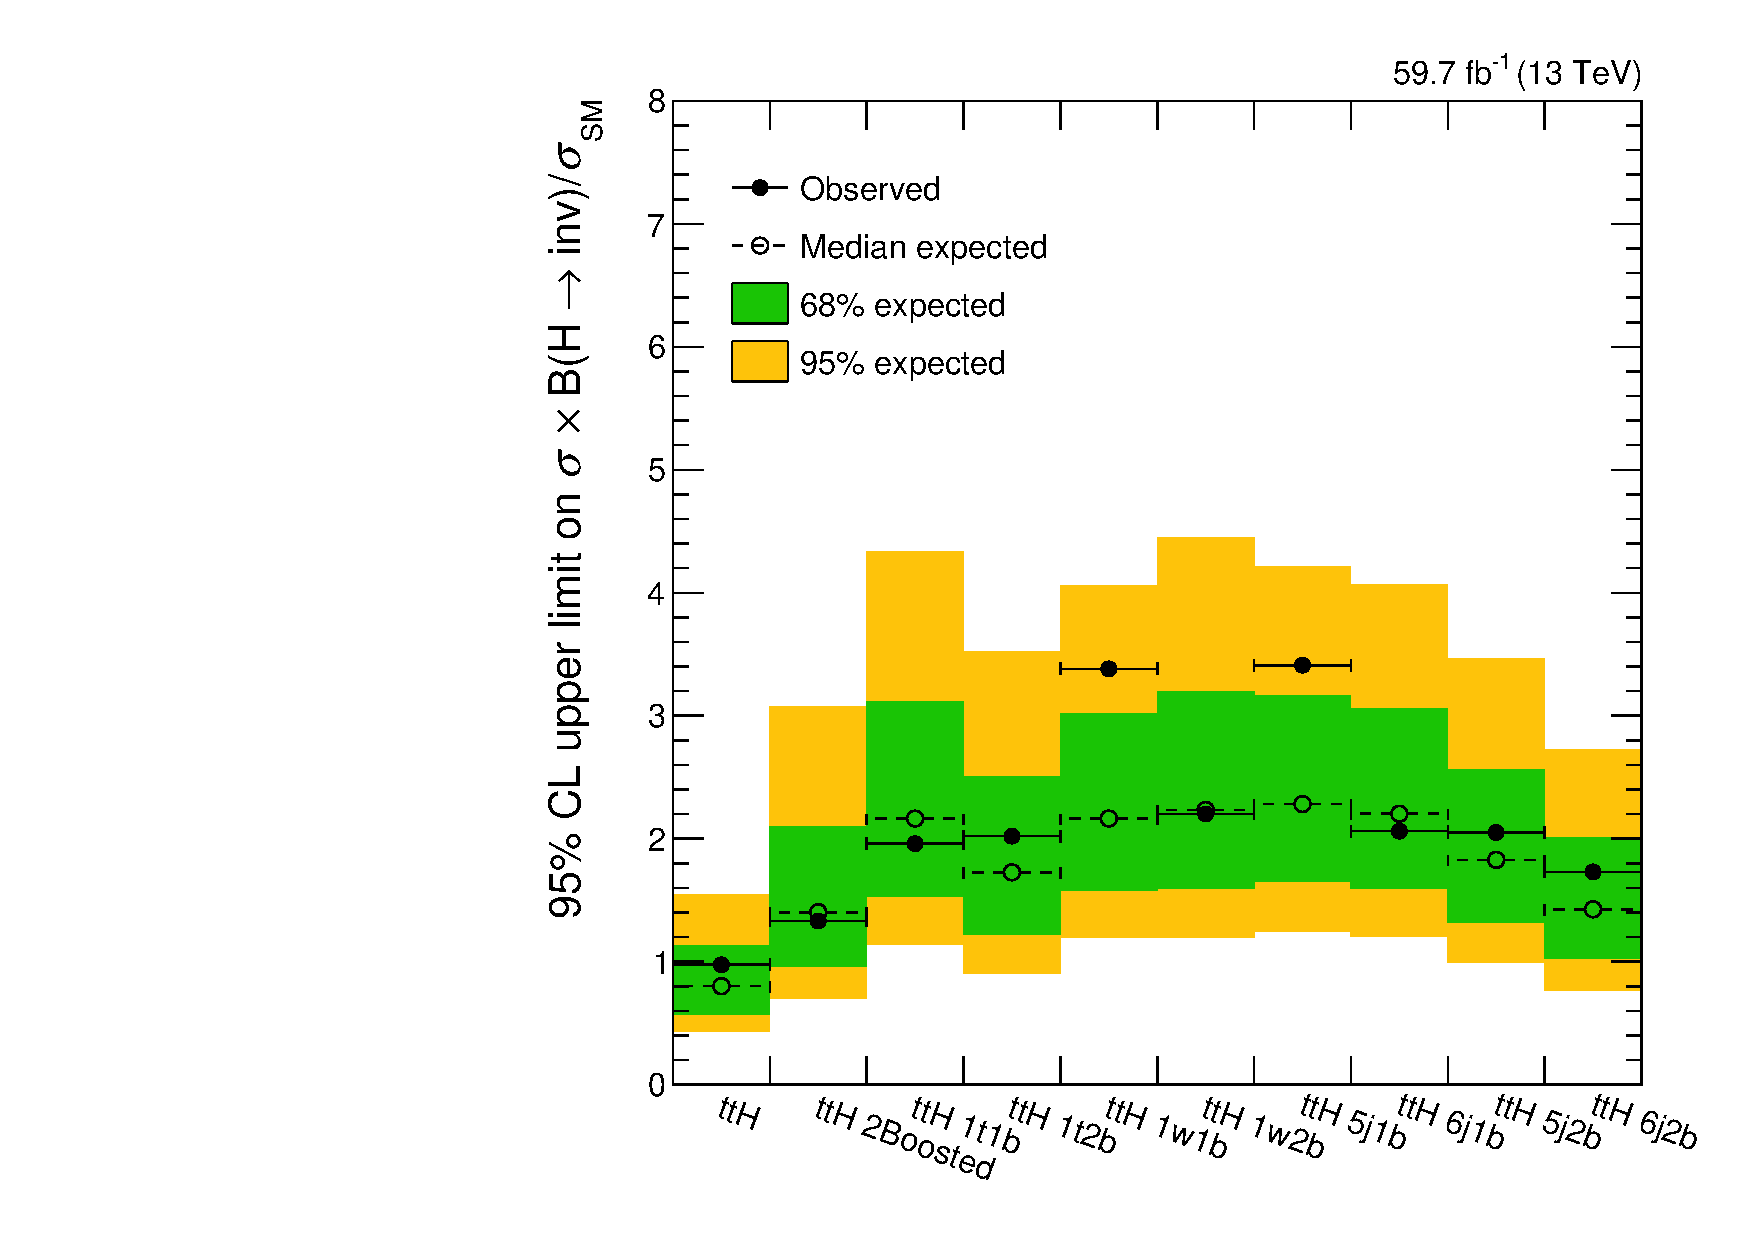
\includegraphics[width=\textwidth]{chapters/higgstoinv/figures/limits/ttH/limit_2018_ttH.pdf}
        \caption{\ttH --- 2018}
    \end{subfigure}
    \caption[Observed and expected 95\,\% CL upper limits on the Higgs boson to invisible state branching fraction in the \ttH category, for both the individual subcategories, and the combination of them, for each data-taking year in Run-2]{Observed and expected 95\,\% CL upper limits on the Higgs boson to invisible state branching fraction in the \ttH category, for both the individual subcategories, and the combination of them, for each data-taking year in Run-2.}
    \label{fig:htoinv_limit_ttH_per_year}
\end{figure}

\begin{figure}[htbp]
    \centering
    \begin{subfigure}[b]{0.45\textwidth}
        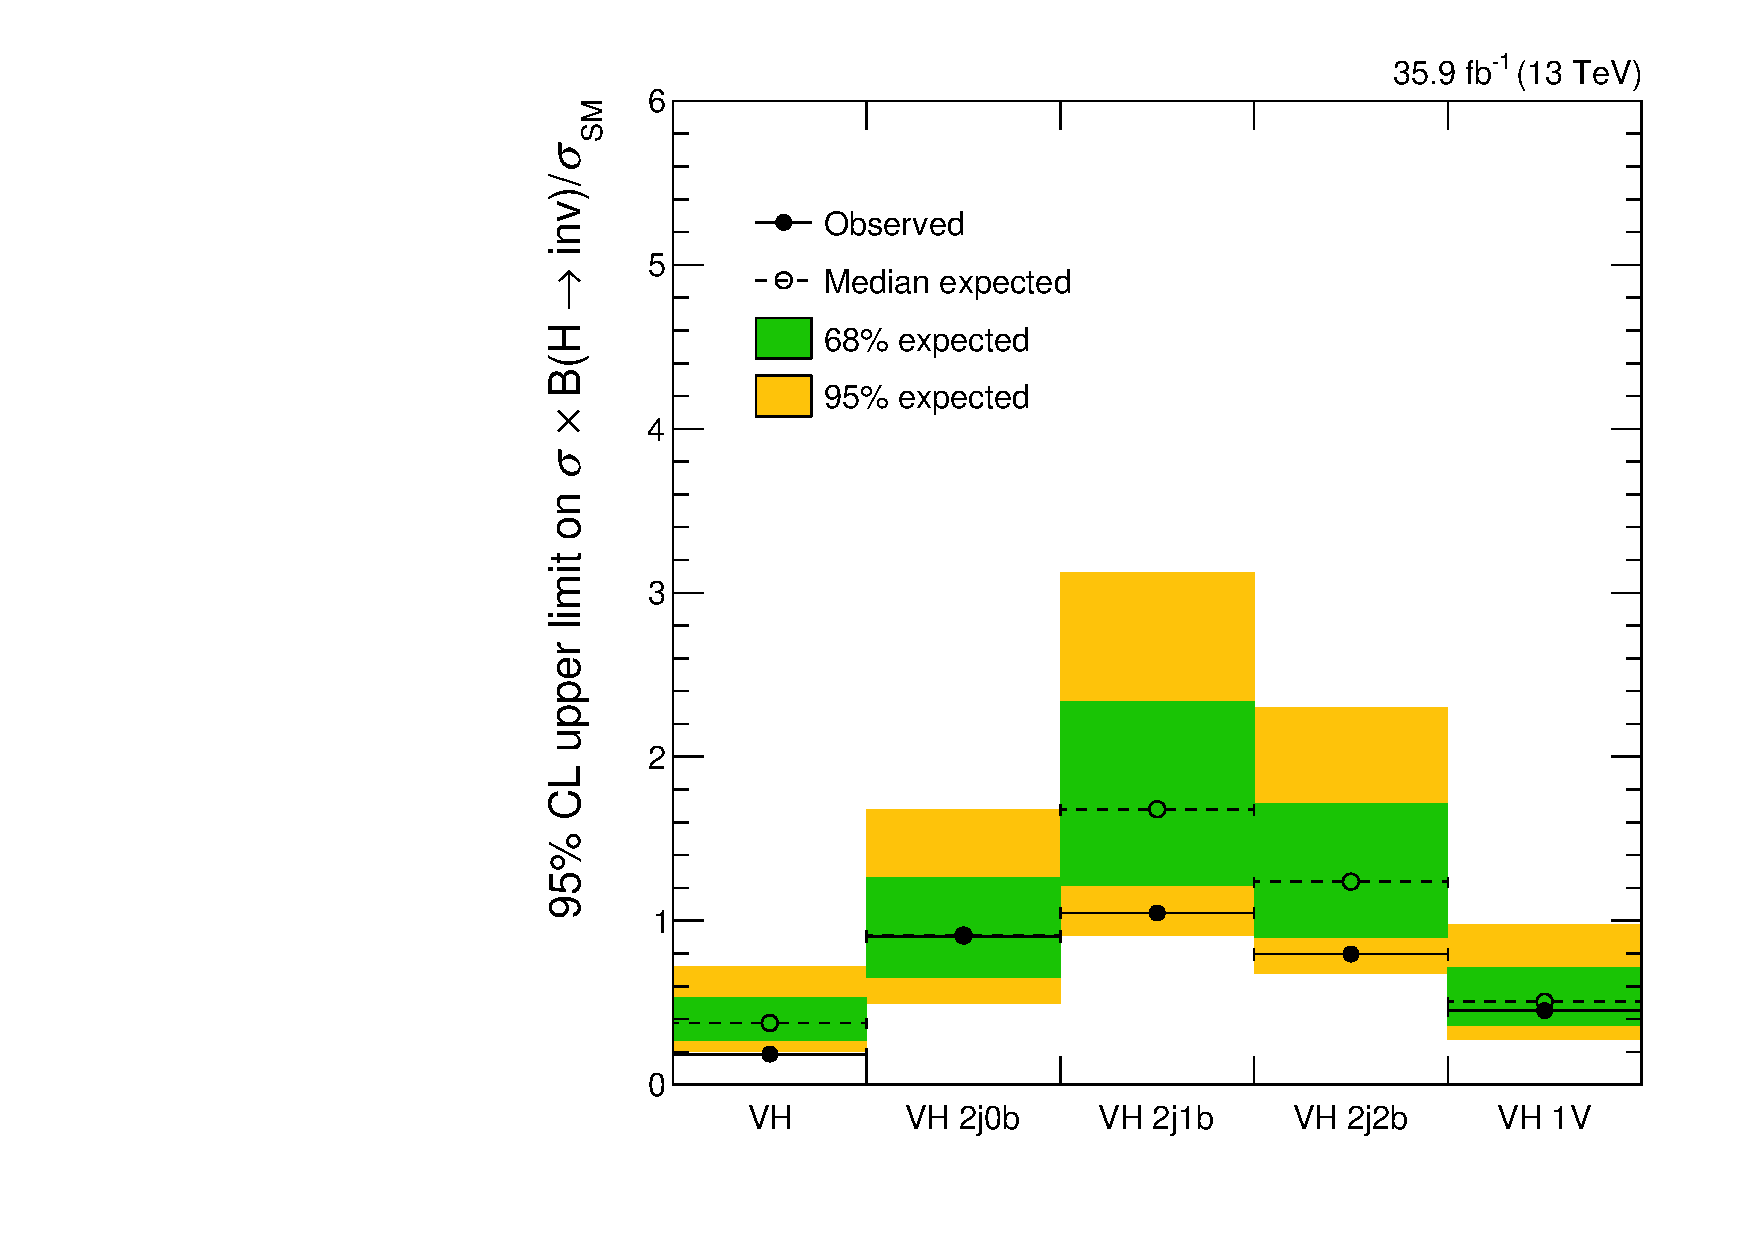
\includegraphics[width=\textwidth]{chapters/higgstoinv/figures/limits/VH/limit_2016_VH.pdf}
        \caption{\VH --- 2016}
    \end{subfigure}
    \hfill
    \begin{subfigure}[b]{0.45\textwidth}
        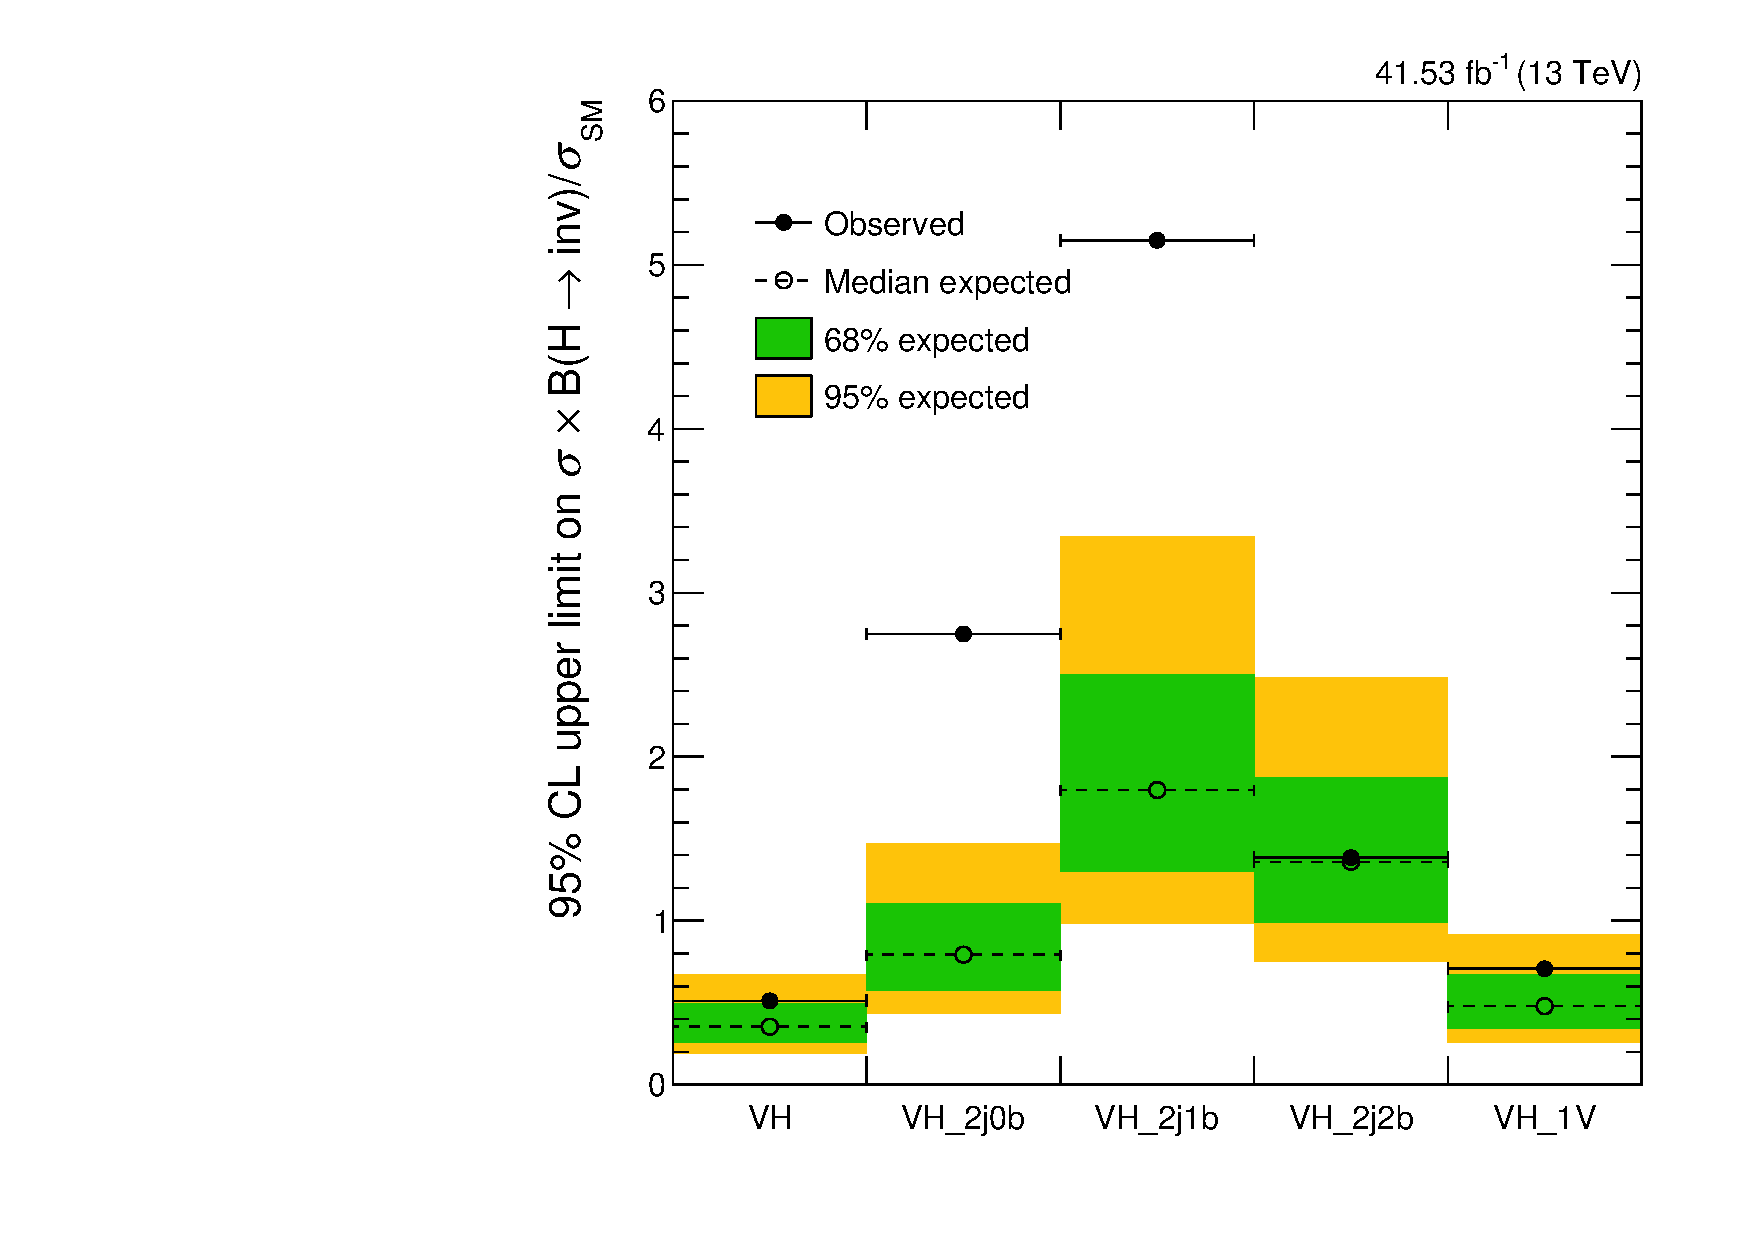
\includegraphics[width=\textwidth]{chapters/higgstoinv/figures/limits/VH/limit_2017_VH.pdf}
        \caption{\VH --- 2017}
    \end{subfigure}

    \begin{subfigure}[b]{0.45\textwidth}
        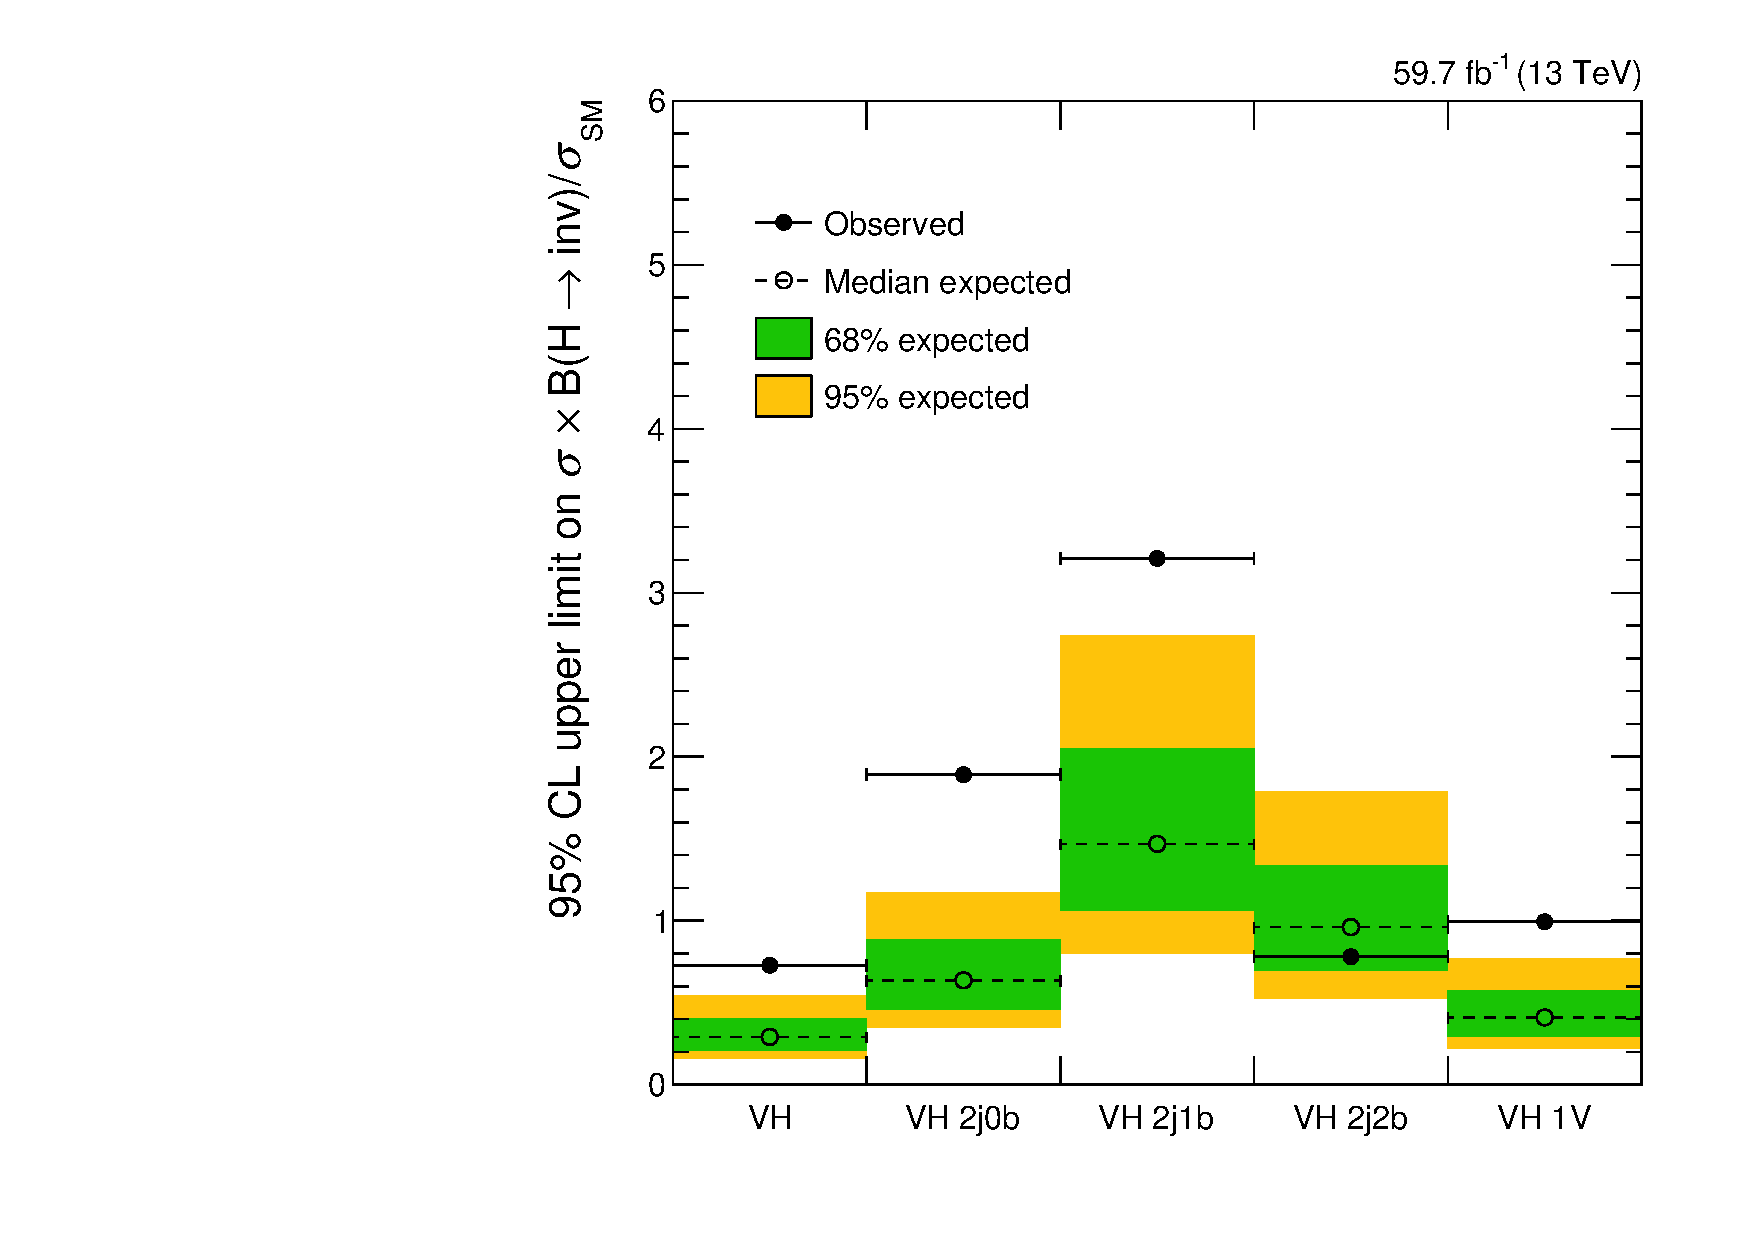
\includegraphics[width=\textwidth]{chapters/higgstoinv/figures/limits/VH/limit_2018_VH.pdf}
        \caption{\VH --- 2018}
    \end{subfigure}
    \caption[Observed and expected 95\,\% CL upper limits on the Higgs boson to invisible state branching fraction in the \VH category, for both the individual subcategories, and the combination of them, for each data-taking year in Run-2]{Observed and expected 95\,\% CL upper limits on the Higgs boson to invisible state branching fraction in the \VH category, for both the individual subcategories, and the combination of them, for each data-taking year in Run-2.}
    \label{fig:htoinv_limit_VH_per_year}
\end{figure}

\clearpage


%=========================================================

\section{Limits and likelihood scans for each year}
\label{sec:limits_likelihoods_year_supplementary}

\begin{figure}[htbp]
    \centering
    \begin{subfigure}[t]{0.45\textwidth}  % top align since figures are same dimensions, but x-axis labels are larger for likelihood
        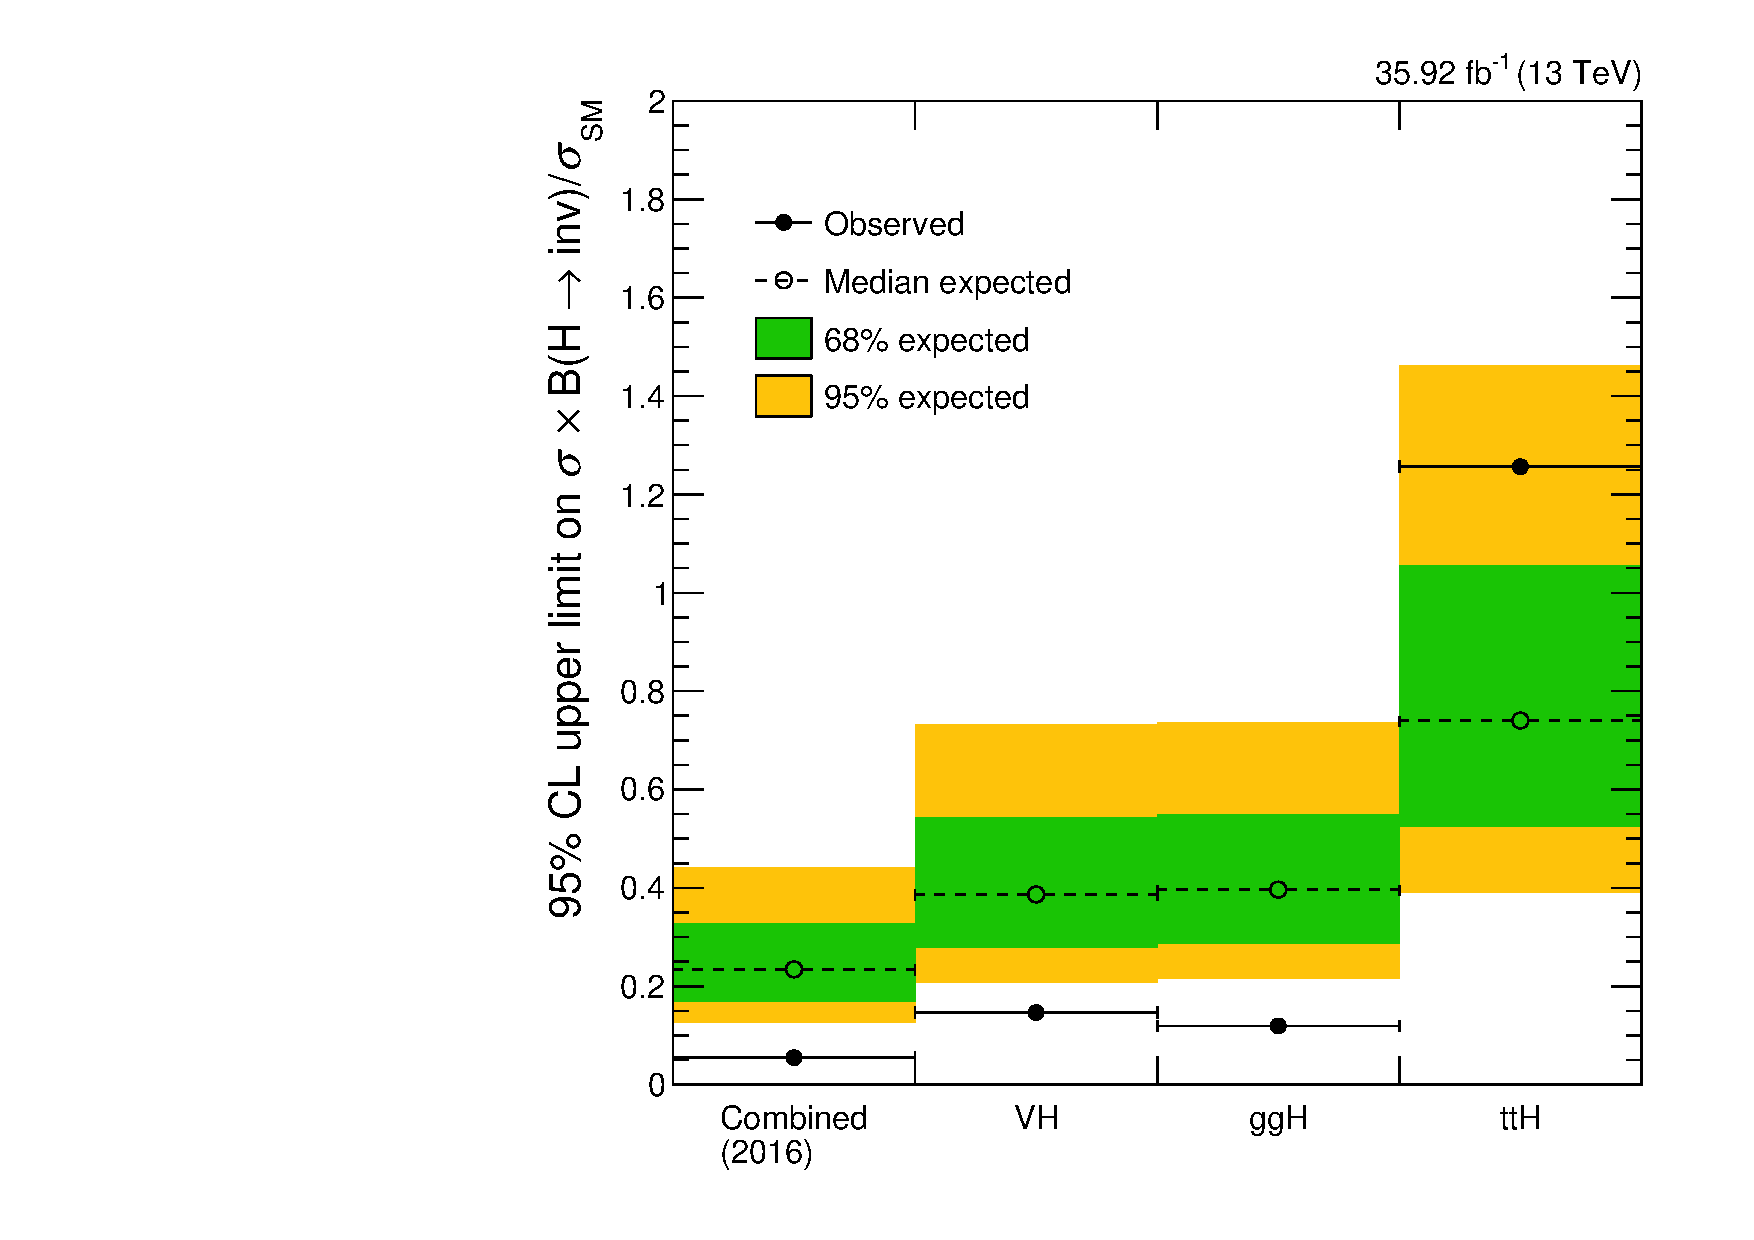
\includegraphics[width=\textwidth]{chapters/higgstoinv/figures/limits/per_year/limit_2016_comb.pdf}
        \caption{Limit --- 2016}
    \end{subfigure}
    \hspace{0.05\textwidth}
    \begin{subfigure}[t]{0.45\textwidth}
        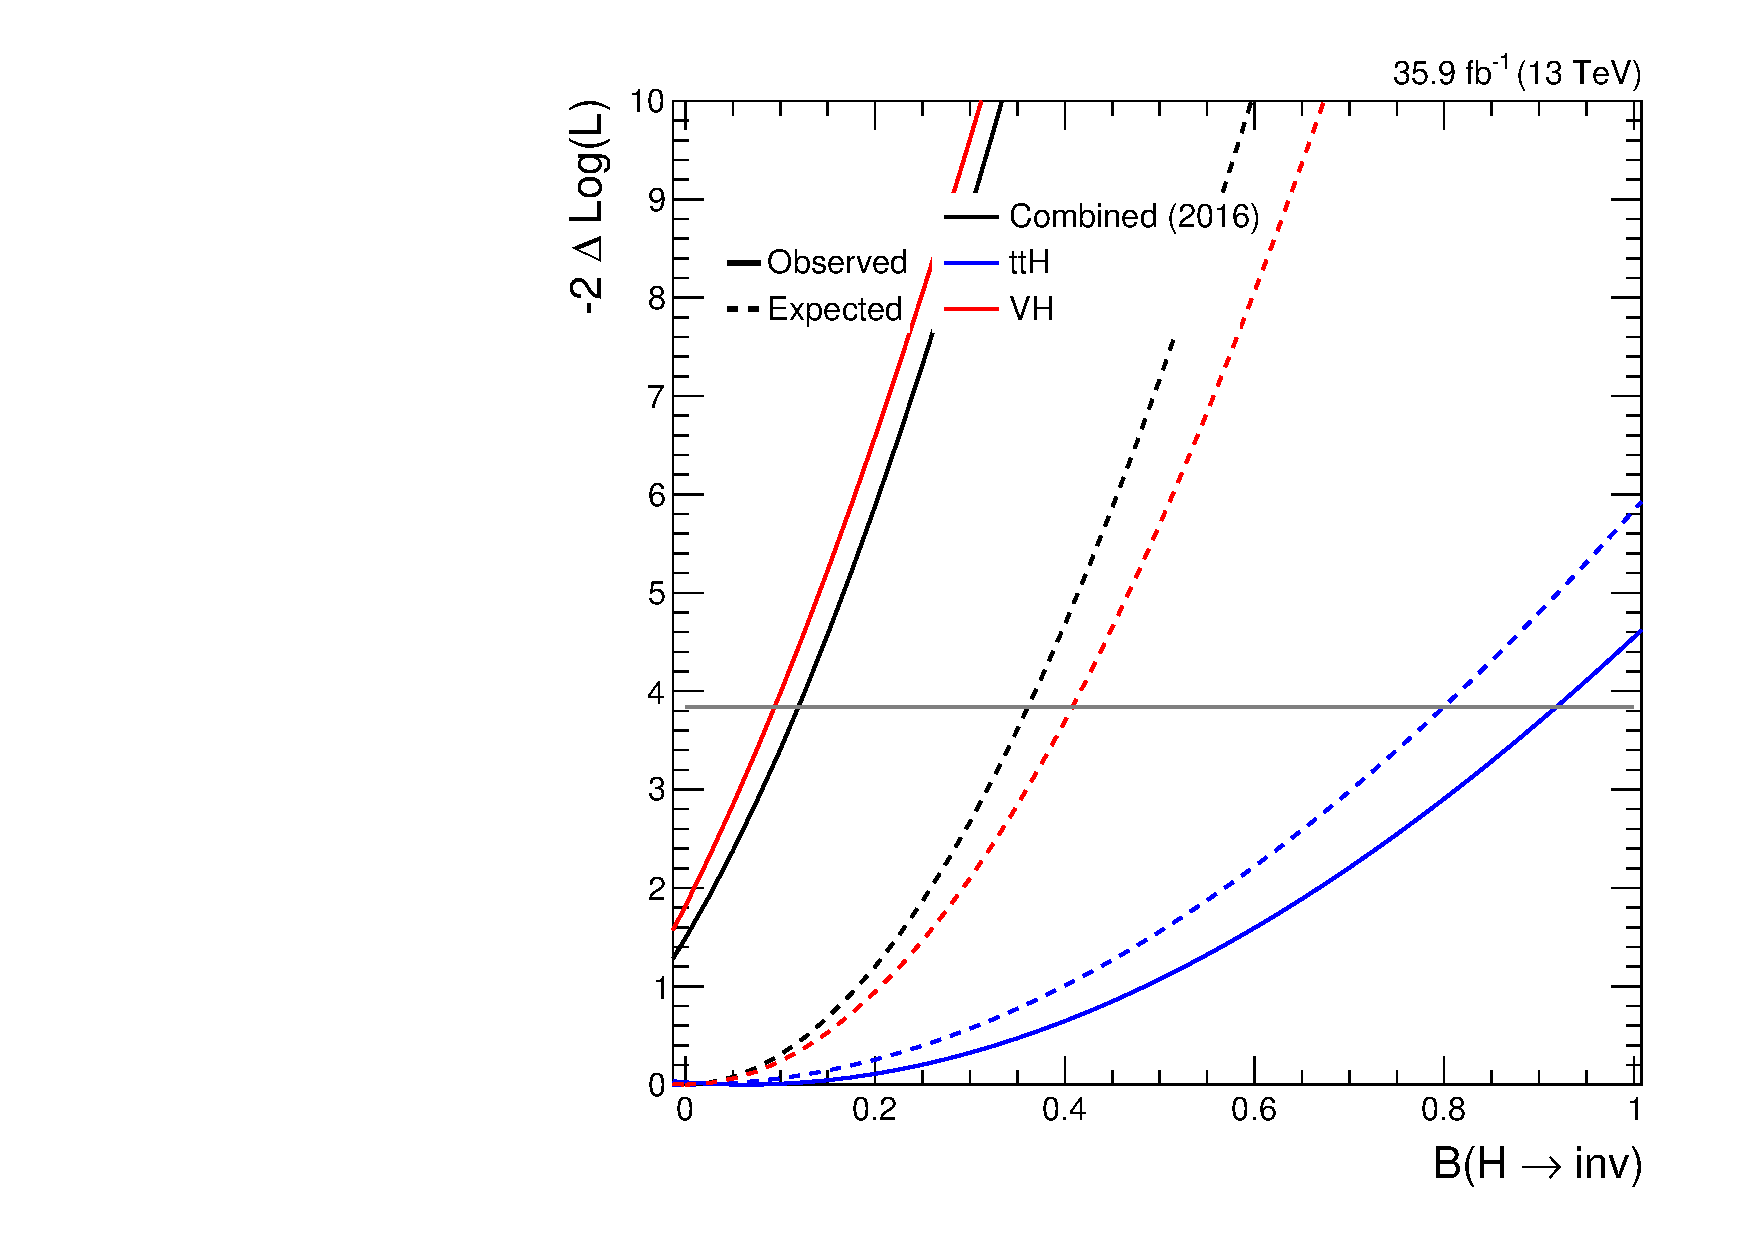
\includegraphics[width=\textwidth]{chapters/higgstoinv/figures/likelihood_scan/profile_likelihood_scan_2016.pdf}
        \caption{Profile likelihood --- 2016}
    \end{subfigure}
    \caption[Observed and expected 95\,\% CL upper limit on the Higgs boson to invisible state branching fraction $\BRof{\higgstoinv}$ and the corresponding profile likelihood ratio as a function of it, for both the individual categories that target a specific production mode, as well as the combination of them, for the 2016 dataset]{Observed and expected 95\,\% CL upper limit on the Higgs boson to invisible state branching fraction $\BRof{\higgstoinv}$ (left) and the corresponding profile likelihood ratio as a function of it (right), for both the individual categories that target a specific production mode, as well as the combination of them, for the 2016 dataset.}
    \label{fig:htoinv_limit_likelihood_2016}
\end{figure}

\begin{figure}[htbp]
    \centering
    \begin{subfigure}[t]{0.45\textwidth}
        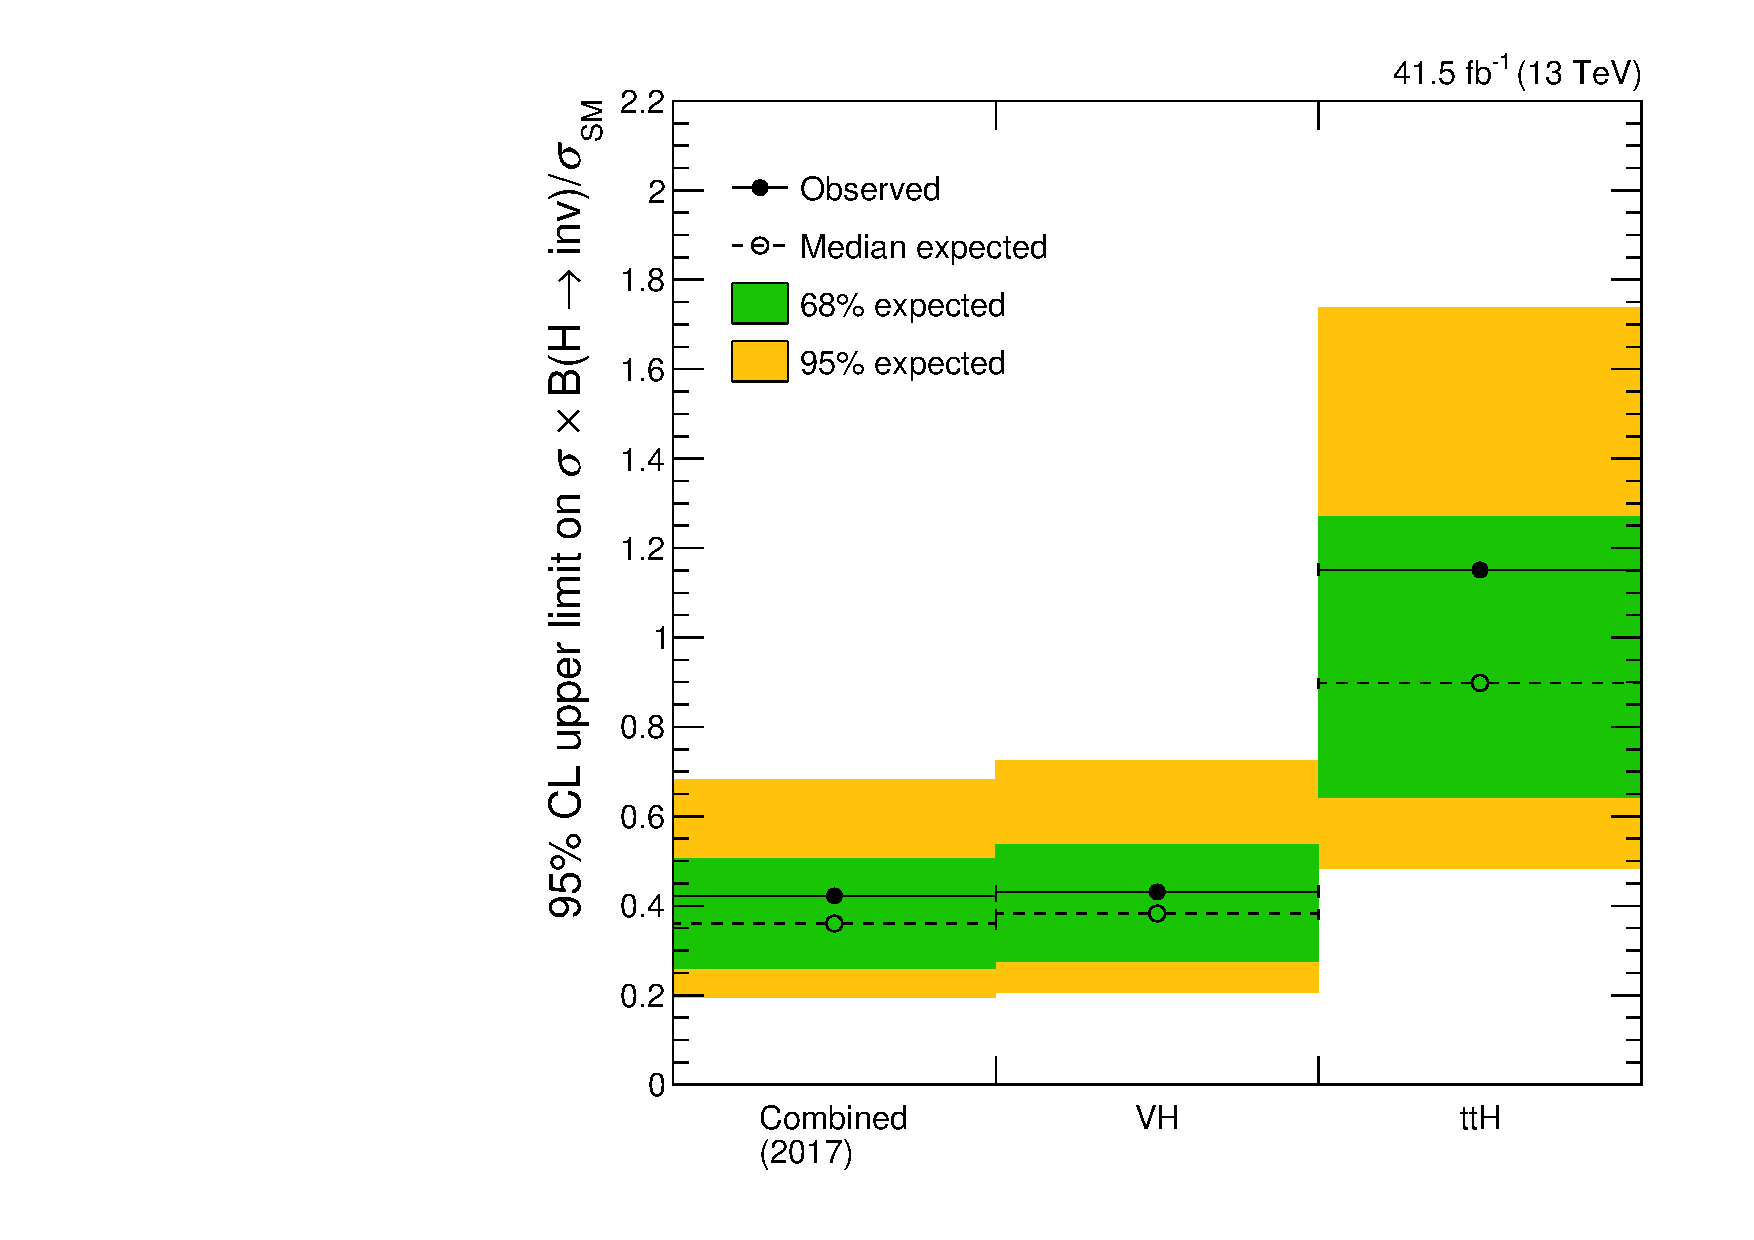
\includegraphics[width=\textwidth]{chapters/higgstoinv/figures/limits/per_year/limit_2017_comb.pdf}
        \caption{Limit --- 2017}
    \end{subfigure}
    \hspace{0.05\textwidth}
    \begin{subfigure}[t]{0.45\textwidth}
        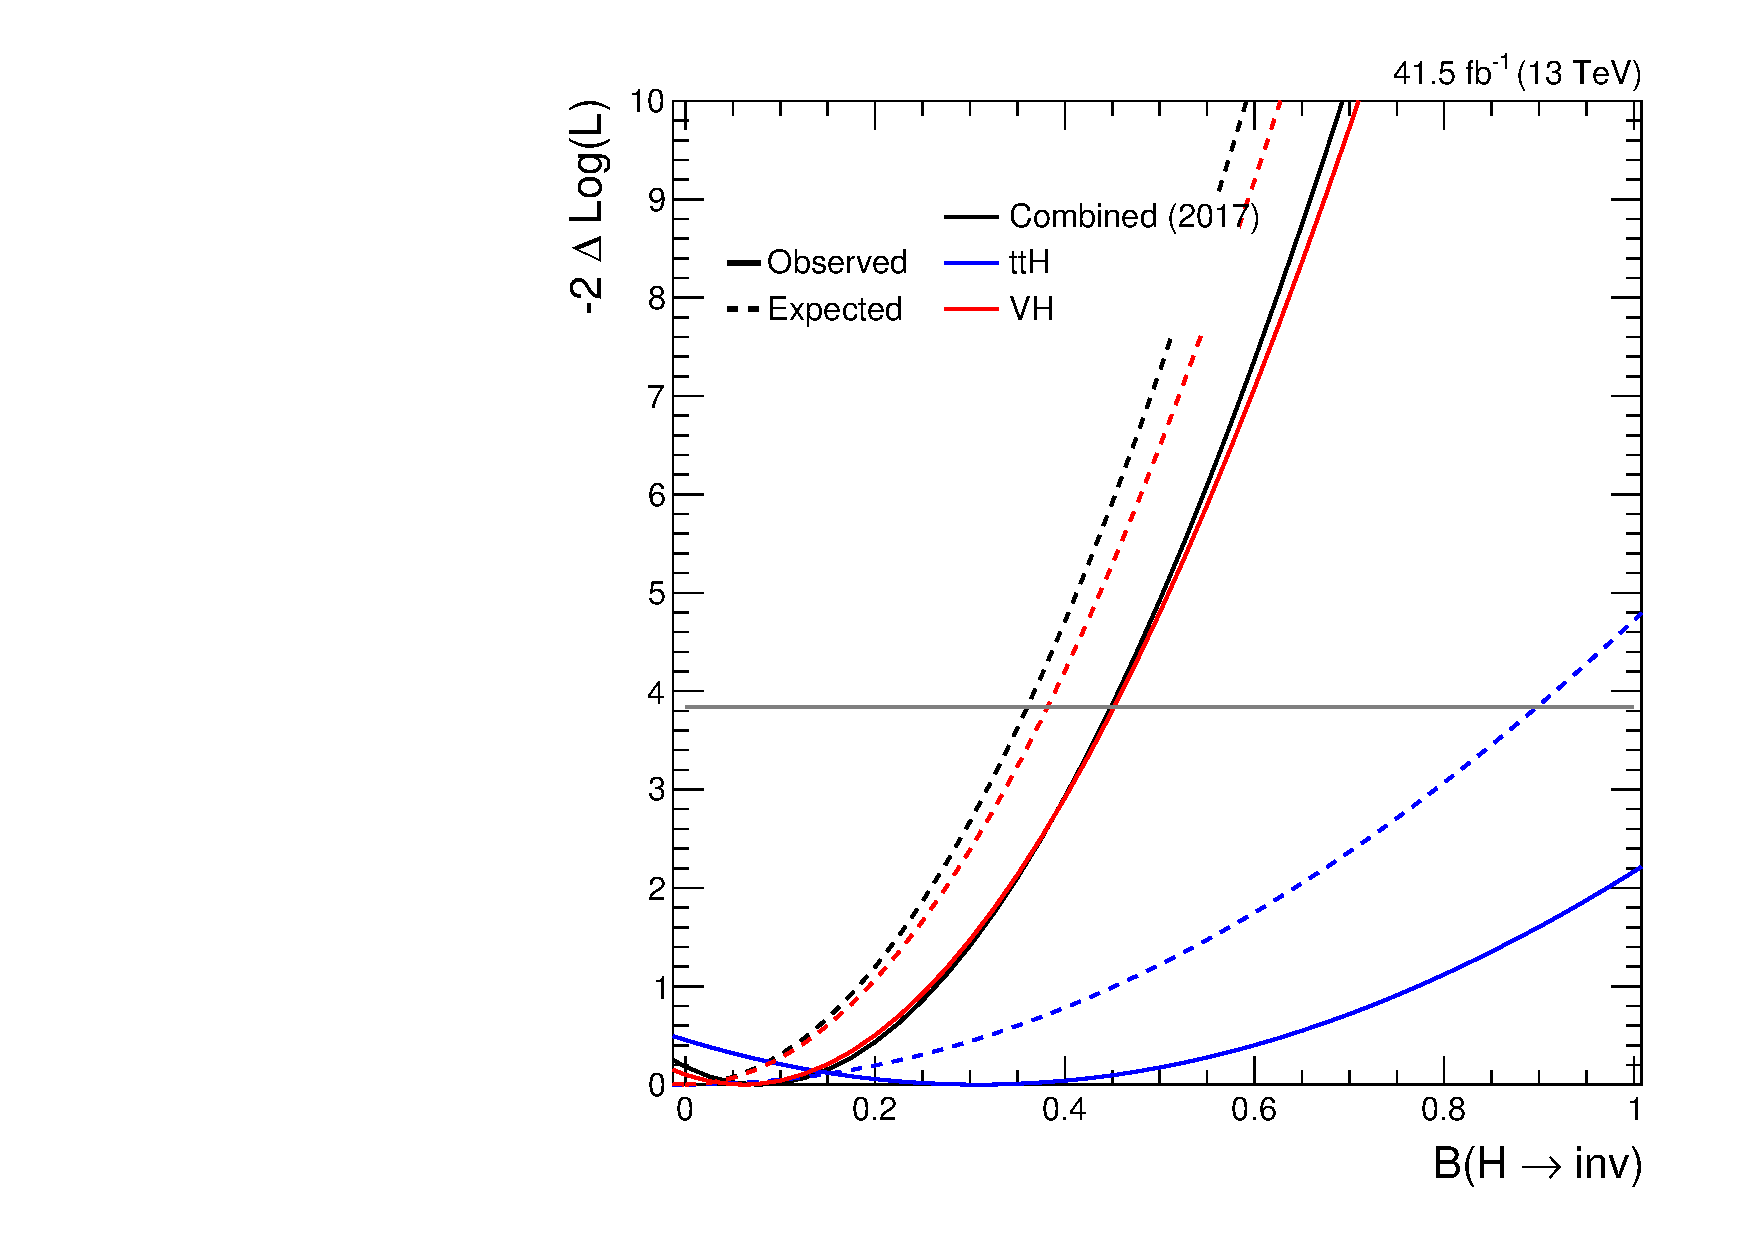
\includegraphics[width=\textwidth]{chapters/higgstoinv/figures/likelihood_scan/profile_likelihood_scan_2017.pdf}
        \caption{Profile likelihood --- 2017}
    \end{subfigure}
    \caption[Observed and expected 95\,\% CL upper limit on the Higgs boson to invisible state branching fraction $\BRof{\higgstoinv}$ and the corresponding profile likelihood ratio as a function of it, for both the individual categories that target a specific production mode, as well as the combination of them, for the 2017 dataset]{Observed and expected 95\,\% CL upper limit on the Higgs boson to invisible state branching fraction $\BRof{\higgstoinv}$ (left) and the corresponding profile likelihood ratio as a function of it (right), for both the individual categories that target a specific production mode, as well as the combination of them, for the 2017 dataset.}
    \label{fig:htoinv_limit_likelihood_2017}
\end{figure}

\begin{figure}[htbp]
    \centering
    \begin{subfigure}[t]{0.45\textwidth}
        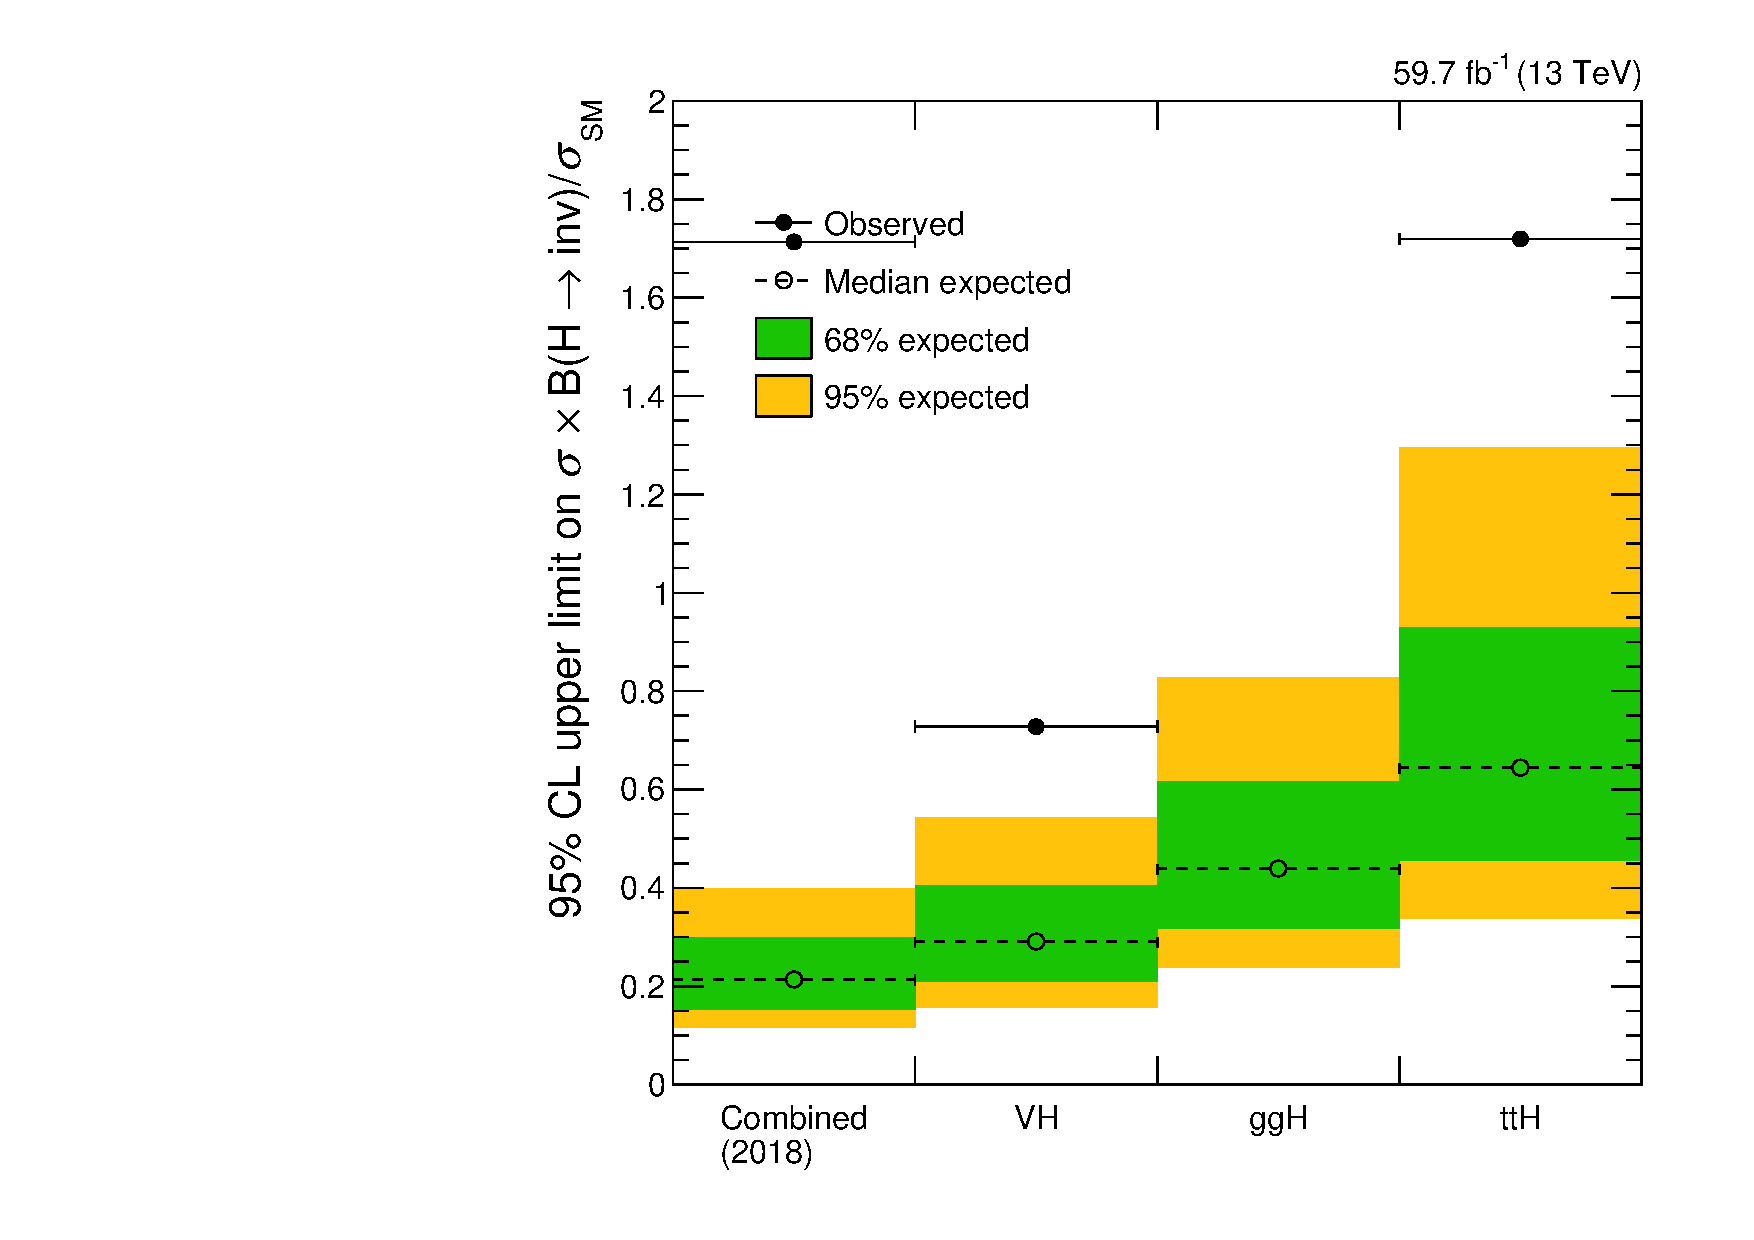
\includegraphics[width=\textwidth]{chapters/higgstoinv/figures/limits/per_year/limit_2018_comb.pdf}
        \caption{Limit --- 2018}
    \end{subfigure}
    \hspace{0.05\textwidth}
    \begin{subfigure}[t]{0.45\textwidth}
        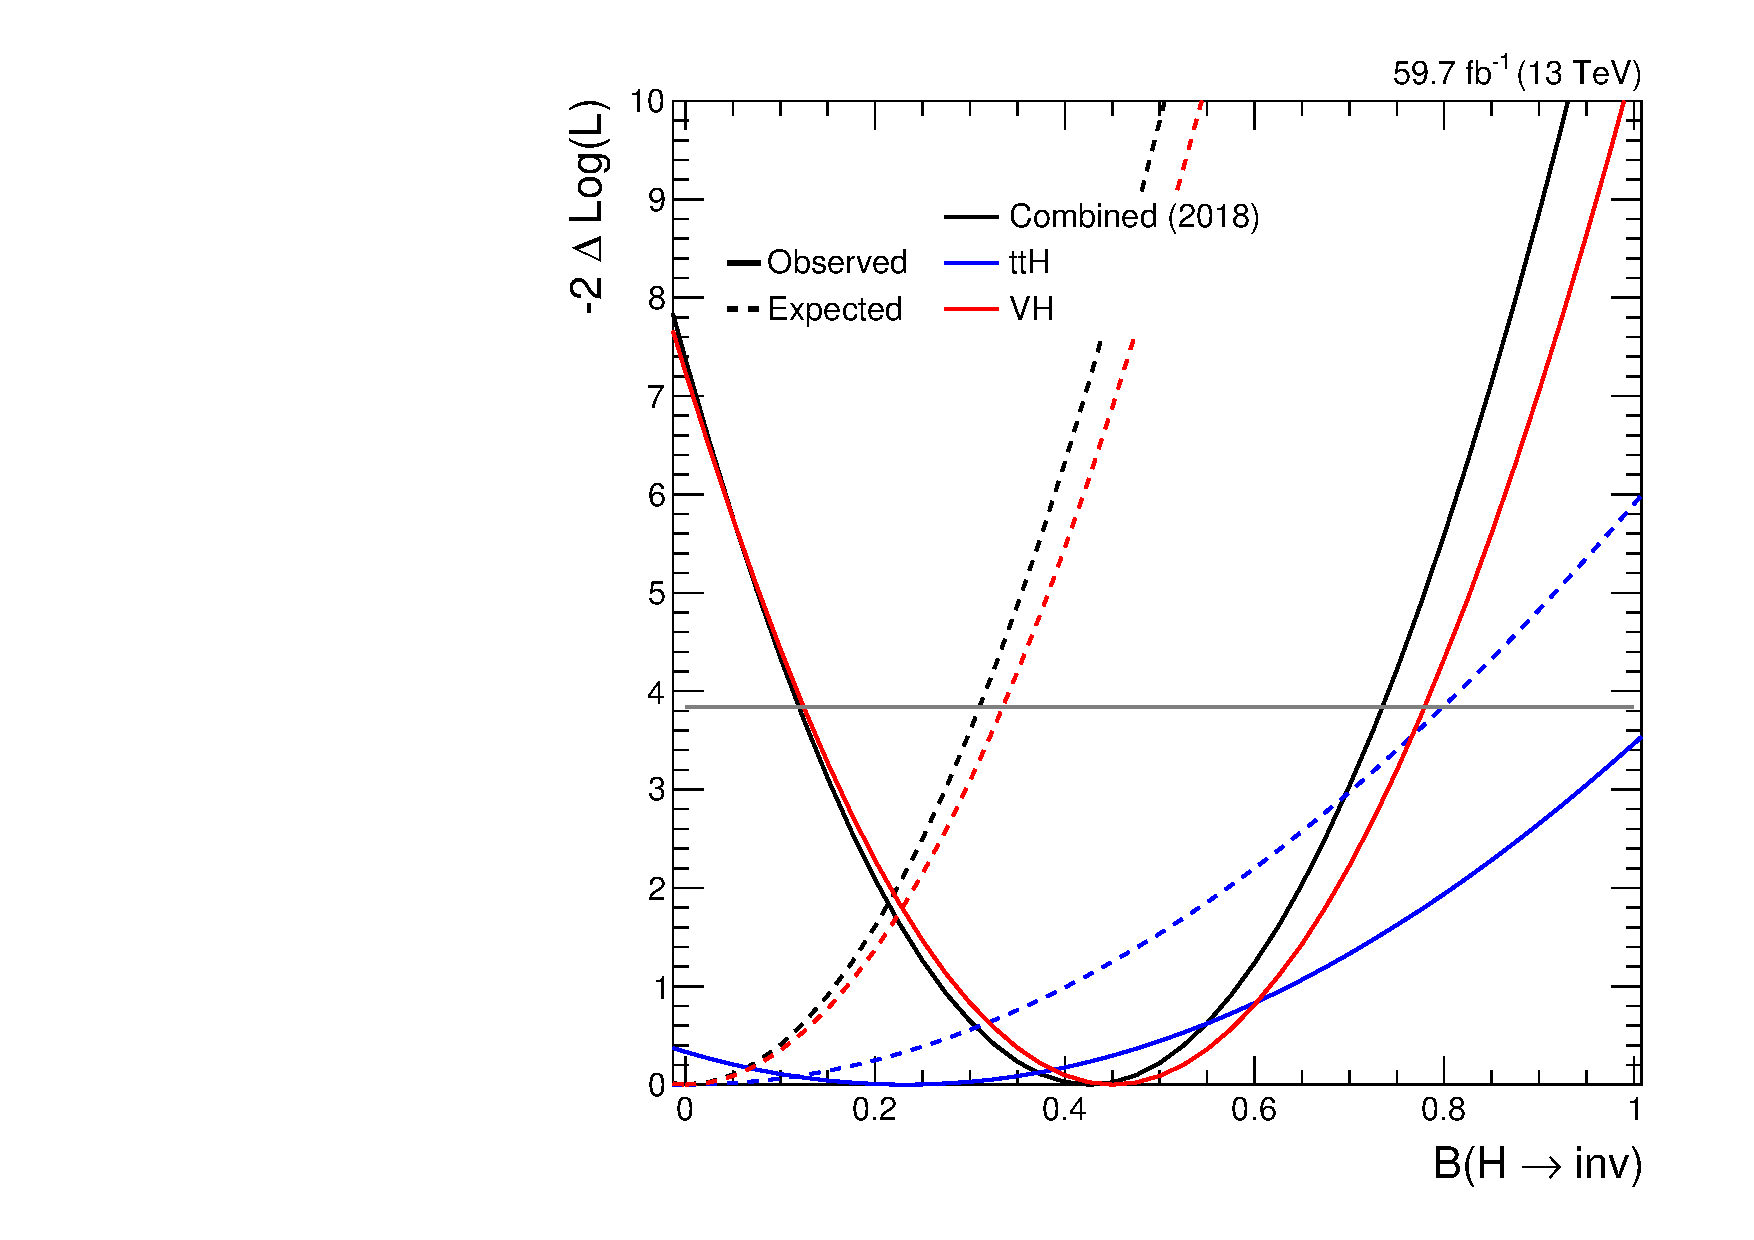
\includegraphics[width=\textwidth]{chapters/higgstoinv/figures/likelihood_scan/profile_likelihood_scan_2018.pdf}
        \caption{Profile likelihood --- 2018}
    \end{subfigure}
    \caption[Observed and expected 95\,\% CL upper limit on the Higgs boson to invisible state branching fraction $\BRof{\higgstoinv}$ and the corresponding profile likelihood ratio as a function of it, for both the individual categories that target a specific production mode, as well as the combination of them, for the 2018 dataset]{Observed and expected 95\,\% CL upper limit on the Higgs boson to invisible state branching fraction $\BRof{\higgstoinv}$ (left) and the corresponding profile likelihood ratio as a function of it (right), for both the individual categories that target a specific production mode, as well as the combination of them, for the 2018 dataset.}
    \label{fig:htoinv_limit_likelihood_2018}
\end{figure}
